	\documentclass{DTEDI_KP}

\usepackage[titles]{tocloft}
\renewcommand\cftfigpresnum{Gambar\ }
\renewcommand\cfttabpresnum{Tabel\  }

\usepackage{hyperref}
\newlength{\mylenf}
\settowidth{\mylenf}{\cftfigpresnum}
\setlength{\cftfignumwidth}{\dimexpr\mylenf+2em}
\setlength{\cfttabnumwidth}{\dimexpr\mylenf+2em}

\usepackage[labelfont=bf]{caption}

\usepackage{caption}
\usepackage{subcaption}
\usepackage{graphicx}
\usepackage{float}
\usepackage{textcomp}
\usepackage{amsmath}

\titleind{KINEMATIKA DAN ANTARMUKA ROBOT SCARA BERBASIS PROCESSSING IDE}

\fullname {IVAN SYAHRONI HERMAWAN}

\idnum {17/415746/SV/13611}

\approvaldate {2 Agustus 2019}

\degree {Teknologi Listrik}

\yearsubmit {2019}

\program {Teknologi Listrik}

\dept {Departemen Teknik Elektro dan Informatika}

\secondsupervisor {Fahmizal,S.T.,M.Sc.}

\secondnip {111198807201609101}

\firstsupervisor {Ma’un Budiyanto,  S.T., M.T.}

\firstnip {197007071999031002}

\begin{document}
	
	\cover
	
	\approvalpage
	
	\preface
	
Puji syukur penulis panjatkan kehadirat Tuhan Yang Maha Esa karena hanya dengan rahmat dan hidayah-Nya, Laporan Kerja Praktik ini dapat diselesaikan tan- pa halangan yang berarti. Keberhasilan dalam menyusun Laporan Kerja Praktik ini tidak lepas dari bantuan berbagai pihak yang mana dengan tulus dan ikhlas membe- rikan masukan guna sempurnanya laporan kerja praktik ini.  Oleh karena itu dalam kesempatan ini, dengan kerendahan hati penulis mengucap terimakasih kepada:
	
	\begin{enumerate}
		\item Bapak Ma’un Budiyanto, S.T., M.T. selaku Ketua Program Studi Teknologi Listrik Universitas Gadjah Mada,
		\item  Bapak Fahmizal, S.T., M.Sc selaku dosen pembimbing pertama yang telah memberikan banyak bantuan, bimbingan, serta arahan dalam Kerja Praktik,
		\item Seluruh Dosen di Teknologi Listrik Sekolah Vokasi Universitas Gadjah Mada, yang tidak bisa disebutkan satu-satu, atas ilmu dan bimbingannya,
		\item Ibu dan Bapak yang selama ini telah sabar membimbing, mengarahkan, dan mendoakan penulis tanpa kenal lelah untuk selama-lamanya, dan
	\end{enumerate}

Penulis menyadari bahwa penyusunan Kerja Praktik ini jauh dari sempurna. Kritik dan saran dapat ditujukan langsung pada e-mail saya. Akhir kata penulis mo- hon maaf yang sebesar-besarnya apabila terdapat kekeliruan di dalam penulisan Kerja Praktik ini.

\vspace{0.1cm}

Wassalamu’alaikum Wr. Wb.

	\begin{tabular}{p{7.5cm}c}
	&Yogyakarta, 2 Agustus 2019\\
	&\\
	&\\
	&\\
	&\\
	&\textbf{Penulis}
	\end{tabular}

\tableofcontents
\addcontentsline{toc}{chapter}{DAFTAR ISI}
\listoftables
\addcontentsline{toc}{chapter}{DAFTAR TABEL}
\listoffigures
\addcontentsline{toc}{chapter}{DAFTAR GAMBAR}

\begin{abstractind}
	%harus diisi nanti
\end{abstractind}

\begin{abstracteng}
	%diisi nanti
\end{abstracteng}

\newpage
\setcounter{page}{1}
\pagenumbering{arabic}

%BAB-1 Laporan KP

\chapter{PENDAHULUAN}

\section{Latar Belakang Masalah}

	Perkembangan teknologi serta ilmu pengetahuan pada masa ke masa semakin berkembang. Perkembangan ini berjalan seiring dengan penelitian-penelitian di berbagai disiplin ilmu khususnya dalam bidang instrumentasi dan kendali. Hal ini dapat dilihat dari banyaknya penggunaan sistem instrumentasi dan kendali dalam dunia industri seperti pengguanaan robot dalam menyelesaiakan pekerjaan manusia.Untuk itu perancangan robot merupakan salah satu solusi untuk memenuhi tuntutan dalam membantu kebutuhan manusia.
	
	Pemilihan robot untuk menggantikan pekerjaan manusia tidak terlepas dengan berbagai kelebihannya. Robot dapat melakukan suatu pekerjaan yang sama dan berulang tanpa merasakan lelah seperti halnya manusia. Pekerjaan ini lah yang biasa ditemukan dalam bidang industri khususnya pada bagian produksi. Robot dengan sistem lengan robot (\emph {robot arm sistem}) merupakan salah satu jenis robot yang dominan berada dalam bidang industri. 
	
	Robot lengan memiliki berbagai jenis, salah satunya adalah robot SCARA (\emph{Selective Compilance Assembly Robot Arm}). Robot SCARA dapat bergerak secara optimal dan efisien karena sebuah persamaan kinematika. Persamaan kinematika yang diguanakan adalah \textit{inverse kinematic} dengan masukan berupa titik koordinat kartesius \textit{($x_{1}$,$y_{2}$)} dan keluaran berupa nilai sudut untuk mengendalikan motor servo pada \textit{shoulder} dan \textit{elbow}.
	
	Dalam mengendalikan sebuah robot, dibutuhkan \textit{platfrom} antar muka sebagai jembatan antara \textit{user} dengan \textit{hardware}. Dalam penelitian ini program antar muka dirancang menggunakan \textit{software} \emph{Processing Ide}. \emph Software ini memiliki beberapa keunggulan yang membuatnya lebih efektif dan cukup mudah untuk digunakan sebagai \textit{platform} antar muka. Keunggulan tersebut salah satunya mudahnya sarana komunikasi terhadap \emph hardware yang digunakan. Oleh Karena itu, pada program kerja praktik ini dilakukan analisis robot SCARA berupa kinematika maju dan kinematika balik dengan perancangan antar muka berbasis \emph {Processing Ide.}\\


\section{Tujuan Penelitian}
Adapun tujuan dalam melaksanakan penelitian "Kinematika dan Antarmuka Robot SCARA Berbasis Processing IDE" adalah sebagai berikut:

	\subsection{Secara Umum}
		\begin{enumerate}
		\item Merancang \emph{ arm manipulator robot} SCARA berbasis Arduino Mega 2560
		\item Memahami dan mengimplementasikan anta muka aplikasi Processing Integrated Development Environment (IDE).
		\item Mengimplementasikan kinematika pada \emph{arm manipulator robot} SCARA.
	\end{enumerate}
	\subsection{Tujuan Khusus}
	 Untuk memenuhi salah satu syarat kelulusan dalam menempuh pendidikan Program   Diploma III Teknologi Listrik, Sekolah Vokasi, Universitas Gadjah Mada. 
	
	
\section{Batasan Penelitian}
	Pembatasan masalah diperlukan untuk mempermudah pelaksanaan penulisan laporan kerja praktik sehingga tidak menyimpang dari judul laporan. Lingkup pembatasan masalah dalam Laporan kerja praktik ini dibatasi pada:
	
	\begin{enumerate}
		
		\item Akurasi dan presisi dari robot lengan dipengaruhi oleh spesifikasi dan torsi dari masing-masing servo pada \textit joint,
		\item  Rancangan mekanik yang sudah tersusun dari awal sehingga tidak dapat diubah lagi. 
		\item Motor DC pada setiap sendi dari \textit joint robot memiliki kebutuhan arus yang berbeda – beda. 
		\item Komunikasi antara Processing IDE dan perangkat menggunakan komunikasi serial.
		
	\end{enumerate}

\section{Metode Kerja Praktik}
Metodologi adalah suatu cara yang digunakan untuk memperoleh data yang akurat, baik melalui observasi lapangan maupun dari \emph datasheet setiap alat yang digunakan. Observasi juga dilakukan dengan meninjau jurnal-jurnal dan konsultasi mengenai penelitian yang dilakukan. Pada bagian ini akan dijelaskan meliputi waktu dan tempat penelitian, alat dan bahan penelitian, rancangan alat, metode penelitian dan prosedur penelitian. Penjelasan lebih rinci tentang metodologi penelitian akan dijelaskan sebagai berikut: 

\begin{enumerate}
	\item Waktu dan Tempat Penelitian \\
	Penelitian dilakukan di Labolatorium Instrumentasi dan Kendali Diploma Teknik Elektro Sekolah Vokasi Universitas Gadjah Mada pada bulan Juli sampai bulan Agustus 20189.
	
	\item Alat dan Bahan \\
	Peralatan yang digunakan dalam Kerja Praktik adalah personal komputer, AC-to-DC Converter 12V, multimeter, Arduino Mega 2560, modul DC-to-DC Converter LM2596, IC TIP 31, Relay Pneumatik, Driver Motor EMS 30A dan catu daya. Sedangkan bahan yang digunakan adalah Motor Servo yang terpasang di setiap \emph joint robot lengan.
	
	\item  Pengumpulan Data \\
	Studi pustaka dilakukan dengan cara mengumpulkan buku-buku, dokumen, serta jurnal-jurnal berbentuk \emph{e-book} yang berkaitan dengan robot lengan. Selain itu, datasheet dari setiap komponen juga ditinjau. Data-data tersebut menjadi referensi untuk merancang, membuat dan menguji alat. 
	
	Konsultasi dilakukan untuk mengumpulkan data melalui tanya jawab atau berdiskusi dengan pihak yang mengetahui dan menguasai segala permasalahan yang dihadapi dalam merancang, membuat, dan menguji robot lengan SCARA. Dalam metode ini penulis berdiskusi dengan dosen pembimbing kerja praktik. 
	
	\item Metode Penelitian \\
	Metode penelitian yang dilakukan meliputi: Pengujian keluaran tegangan catu daya, pengujian kinerja motor DC, pengujian konfigurasi driver motor H – Bridge, pengujian \emph{Graphical User Interface }(GUI) pada Processing IDE, pengujian perhitungan kinematika balik, pengujian kinematika maju,  serta pengambilan data dan analisa data.
	
	\item Prosedur Penelitian\\
	Prosedur penelitian adalah langkah-langkah dalam menyelesaikan kerja praktik yang akan disajikan dalam bentuk diagram alir. Berikut adalah gambar diagram alir prosedur penelitian yang disajikan pada gambar...
\end{enumerate}

\section{Sistematika Penulisan}
Penulisan laporan kerja praktik ini dilakukan dengan mengikuti sistematika sebagai berikut :\\
\noindent
\textbf{BAB I\hspace*{0.6cm}: PENDAHULUAN}\\
\noindent
Memuat latar belakang masalah,tujuan, dan maksud,batasan masalah, metodologi penetilian, dan sistematika penulisan.\\
\noindent
\textbf{BAB II\hspace*{0.5cm}: LANDASAN TEORI}\\
\noindent
Memuat gambaran umum SCARA, \textit{invers kinematic} dengan analisis Denavit-Hartenberg, Software LabVIEW,dan Arduino Mega 2560.\\
\textbf{BAB III\hspace*{0.375cm}:  PERANCANGAN SISTEM}\\
\noindent
Memuat perancangan sistem secara umum, meliputi perancangan dari segi elektronis dan software dari robot Serpent-1.\\
\textbf{BAB IV\hspace*{0.4cm}: PENGUJIAN SISTEM}\\
\noindent
Memuat pengujian dan analisis kerja dari sistem aktuator dan sensor dari Serpent, serta pengujian sistem secara keseluruhan.\\
\textbf{BAB V\hspace*{0.6cm}: PENUTUP}\\
Memuat kesimpulan dari perancangan, pembuatan, pengujian, dan analisis kerja robot Serpent-1, serta berisi saran-saran untuk pengembangan lebih lanjut.\\
%BAB_2 LAPORAN KP
\chapter{LANDASAN TEORI}

\section{Gambaran Umum Robot Lengan}

Robot adalah adalah sebuah alat yang terdiri dari gabungan mekanik dan elektronik yang dapat melakukan tugas fisik, baik menggunakan pengawasan dan kendali manusia maupun secara otomatis. Robot dapat melakukan suatu tugas secara berulang tanpa merasa lelah sehingga robot banyak digunakan dalam dunia industri khususnya pada bidang produksi. Salah satu jenis robot yang sering digunakan dalam bidang produksi adalah sistem lengan robot.

Robot lengan adalah robot yang memiliki bentuk fisik seperti halnya lengan pada manusia dan memiliki derajat kebebasan (\emph{Degre of Freedom}) tertentu bergantung pada jumlah sendi yang digunakan. Robot lengan pada bidang industri biasa digunakan sebagai aktuator untuk mengambil dan meletakkan suatu objek secara terus menerus.
	

Pada umumnya struktur robot lengan terdiri dari beberapa bagian.  Bagian utama dari robot lengan adalah struktur mekanik ({Manipulator}) yang merupakan susunan kerangka yang tidak dapat digerakkan (\emph{Rigid}) dan lengan (\emph{Link}) yang satu sama lain terhubung oleh sendi (\emph {joint}). Dengan adanya \emph{joint} yang menghubungkan dua \emph{link} menjadi satu kesatuan sehingga \emph{joint} membentuk satu derajat kebebasan. Jika diibaratkan dengan tubuh manusia, \emph{link} adalah tulang sedangkan \emph{joint} adalah sendi-sendinya. \emph{Joint} memiliki dua pergerakan, yaitu pergerakan \emph{revolute joint} (gerak berputar) dan \emph{prismatic joint} (gerak bergeser). Jenis-jenis dari pergerakan \emph{joint} ditunjukkan pada Gambar 2.1.

	\begin{figure}[H]
	\centering
	\includegraphics[width=11cm]{gambar/joint.png}
	\caption{Jenis-Jenis \emph Joint}
\end{figure}
Pada ujung pangkal lengan, robot lengan umumnya menggunakan \emph{gripper} yang dapat dipakai untuk memindahkan suatu objek. Robot lengan dalam menjalankan tugasnya dikontrol menggunakan sensor serta aktuator yang telah dirancang untuk melakukan tugas sesuai dari yang diperintahkan. Perpaduan antara sensor dan aktuator ini yang menyebabkan robot lengan dapat bekerja secara optimal dan presisi.

\subsection{\emph{Degress of Freedom }}
\emph{Degress of Freedom} (DOF) merupakan sebuah konfigurasi yang dapat meminimalkan spesifikasi dengan menggunakan parameter yang dapat menyatakan posisi suatu sistem pada setiap saat. Umumnya robot lengan mempunyai paling sedikit enam independen derajat kebebasan, tiga derajat kebebasan untuk translasi dan tiga derajat kebebasan untuk rotasi. Robot lengan paling tidak memiliki tiga derajat kebebasan untuk dapat memiliki \emph{workspace} yang cukup. \emph{Workspace} dari sebuah robot lengan merupakan total volume yang dapat dijangkau oleh \emph{end-effector} dari pergerakan semua \emph{joint}-nya dari titik minimum hingga maksimum. 

\subsection{Konfigurasi Robot Lengan}
Pada dasarnya berbagai jenis dari robot lengan dapat dibedakan dari konfigurasinya. Konfigurasi robot lengan merupakan perpaduan antara pergerakan \emph{joint} yang dimiliki oleh robot lengan. Konfigurasi ini memiliki tipe yang berbeda-beda sehingga \emph {workspace} yang dimiliki pada tiap robot lengan pasti berbeda.

\subsubsection{Konfigurasi \emph{Articulated} (\emph{Revolute - Revolute - Revolute)}} 
\emph{Articulated} manipulator ini pada dasarnya mempunyai jenis \emph{revolute joint} pada ketiga \emph{joint} robot lengan (\emph {base, shoulder, elbow}). Dengan konfigurasi ini, robot lengan dengan konfigurasi \textit{Articulated} dapat memiliki variasi DOF yang banyak. DOF yang dapat dihasilkan dengan robot lengan dengan konfigurasi seperti ini adalah tiga DOF hingga sampai dengan enam DOF tergantung dari kebutuhan dan fungsi yang akan dilakukan oleh robot lengan. Konfigurasi dari \textit{joint revolute} ini menjadikan robot lengan jenis ini mempunyai kebebasan yang besar dari pergerakannya dalam ruang yang kecil sehingga menjadikan jenis konfigurasi \textit{Articulated} manipulator ini banyak dipakai dan memiki desain yang populer. Konfigurasi \textit{Articulated} ini ditunjukkan pada Gambar 2. 2.
	\begin{figure}[H]
	\centering
	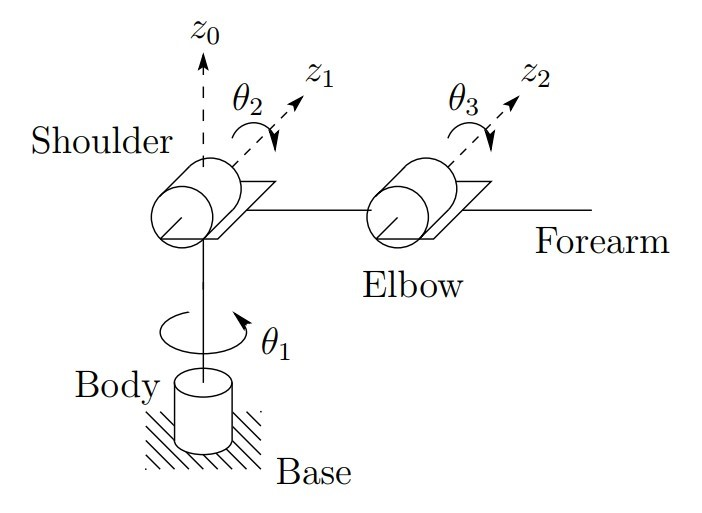
\includegraphics[width=8cm]{gambar/articulated.jpg}
	\caption{Struktur dari Konfigurasi  \textit{Articulated}}
\end{figure}
\subsubsection{Konfigurasi \textit{Spherical} (\textit{Revolute – Revolute – Prismatic})} 

Konfigurasi \textit{Spherical} merupakan konfigurasi yang mempunyai dua buah \textit{joint revolute} dan satu buah \textit{joint prismatic}. \textit{Joint prismatic} berada ini \textit{joint} ketiga atau pada bagian \textit{elbow}. Sementara dua \textit{joint} lainnya berada di \textit{shoulder} dan \textit{wrist}. Sruktur dari konfigurasi \textit{Spherical} ditunjukkan pada Gambar 2.3.
	\begin{figure}[H]
	\centering
	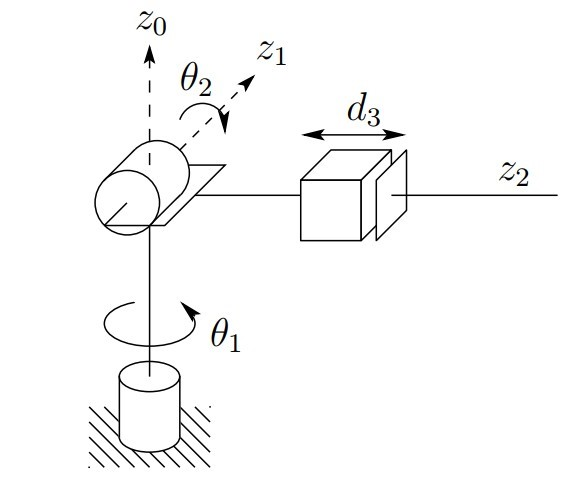
\includegraphics[width=8cm]{gambar/spherical.jpg}
	\caption{Struktur dari Konfigurasi \textit{Sperical}}
\end{figure}


\subsubsection{Konfigurasi SCARA (\textit{Revolute – Revolute – Prismatic}) } 

Konfigurasi \textit{Selective Compliant Articulated Robot for Assembly} (SCARA) merupakan konfigurasi yang mempunyai dua buah \textit{joint revolute} dan satu buah \textit{joint prismatic} sama seperti konfigurasi \textit{Spherical}. Meskipun SCARA memiliki struktur \textit{joint revolute – revolute – prismatic} (RRP) sama seperti konfigurasi yang dimiliki \textit{Spherical}, struktur ini sedikit berbeda dengan konfigurasi \textit{Spherical} dari tampilannya maupun dari jarak \textit{workspace} nya. Tidak seperti konfigurasi \textit{Spherical}, dimana z0 tegak lurus terhadap 1, dan z1 tegak lurus dengan z2, konfigurasi SCARA memiliki struktur z0, z1, dan z2 yang paralel. Struktur dari konfigurasi SCARA ditunjukkan pada Gambar 2.4.
	\begin{figure}[H]
	\centering
	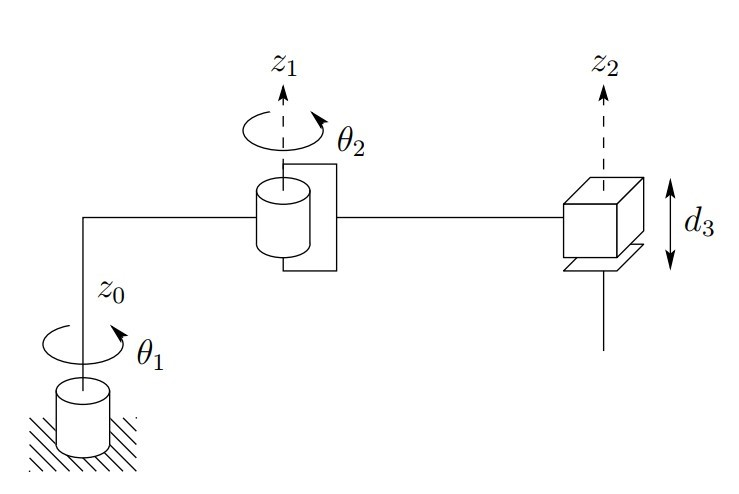
\includegraphics[width=8cm]{gambar/scara.jpg}
	\caption{Struktur dari Konfigurasi SCARA}
\end{figure}

\subsubsection{Konfigurasi \textit{Cylindrical} (\textit{Revolute – Prismatic – Prismatic}) } 

Konfigurasi \textit{Cylindrical} merupakan konfigurasi yang mempunyai satu buah \textit{joint revolute} dan dua buah \textit{joint prismatic}. \textit{Joint revolute} menghasilkan pergerakan rotasi di \textit{base}, sementara \textit{joint prismatic} berada di bagian \textit{shoulder} dan \textit{elbow}. Struktur dari konfigurasi \textit{Cylindrical} ditunjukkan pada Gambar 2.5
	\begin{figure}[H]
	\centering
	\includegraphics[width=4cm]{gambar/cylindrical.jpg}
	\caption{Struktur dari Konfigurasi \textit{Cylindrical}}
\end{figure}
\subsubsection{Konfigurasi \textit{Cartesian} (\textit{Prismatic – Prismatic – Prismatic})  } 

Konfigurasi \textit{Cartesian} mempunyai tiga buah \textit{joint prismatic}. Variabel \textit{joint} dari konfigurasi \textit{prismatic} adalah koordinat \textit{Cartesian} dari \textit{end-effector} dengan memperhatikan letak \textit{base} dari robot lengan. Kinematika dari jenis konfigurasi ini adalah yang paling sederhana dari semua konfigurasi robot lengan. Konfigurasi \textit{Cartesian} sangat berguna untuk penyusunan suatu barang di bidang datar seperti mesin laser, kargo atau memindahkan barang. Struktur dari konfigurasi \textit{Cartesian} ditunjukkan pada Gambar 2.6.

	\begin{figure}[H]
	\centering
	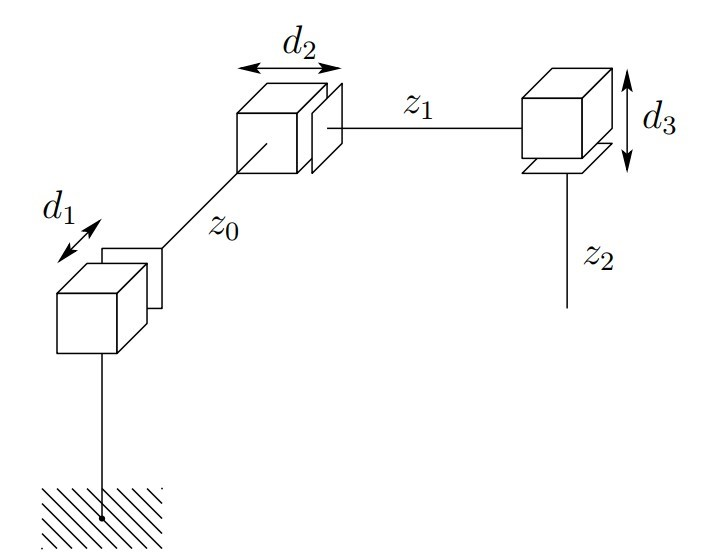
\includegraphics[width=7cm]{gambar/cartesian.jpg}
	\caption{Struktur dari Konfigurasi \textit{Cartesian}}
\end{figure}

\subsection{ \textit{Wrist} dan \textit{End-effector} }

\textit{Wrist} atau pergelangan tangan merupakan \textit{joint} diantara lengan dan \textit{end-effector}. \textit{Joint wrist} ini pada umumnya terdapat \textit{joint revolute} . Hal ini umum digunakan pada desain manipulator lengan dengan konfigurasi \textit{Spherical}. Konfigurasi \textit{Spherical} mempunyai \textit{joint revolute} yang saling berpotongan diantara ketiganya, maksudnya setiap \textit{joint} berputar sesuai koordinat x, y dan z. Rotasi atau perputaran dengan \textit{axis} sumbu x adalah \textit{roll}, perputaran dengan \textit{axis} sumbu y adalah \textit{pitch} dan perputaran dengan \textit{axis} sumbu z adalah \textit{yaw}. \textit{Joint spherical wrist} ini dijelaskan pada Gambar 2. 7.
	\begin{figure}[H]
	\centering
	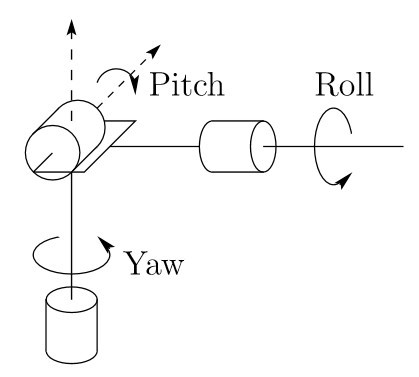
\includegraphics[width=6cm]{gambar/wirst.jpg}
	\caption{Struktur dari \textit{Joint Spherical Wrist}}
\end{figure}


\textit{End-effector} merupakan perangkat atau alat yang terhubung dengan ujung lengan robot. \textit{End-effector} adalah bagian robot yang berhubungan langsung dengan objek. Struktur, pergerakan, material dari \textit{end-effector} bergantung pada tugas yang akan dilakukan robot tersebut. Stuktur dan bentuk dari \textit{end-effector} ditunjukkan pada Gambar 2.8.
	\begin{figure}[H]
	\centering
	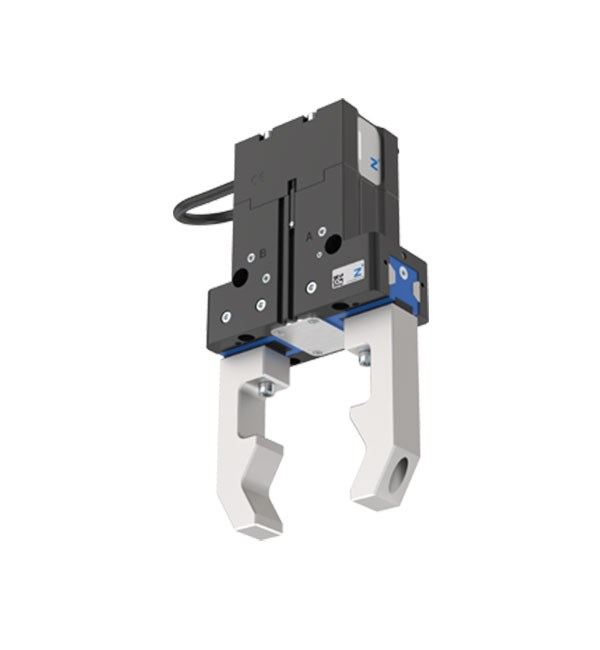
\includegraphics[width=6cm]{gambar/end_effector.jpg}
	\caption{Struktur \textit{End-Effector}}
	\end{figure}


\section{Kinematika}
Kinematika merupakan pembelajaran pergerakan tubuh robot tanpa memperhitungkan gaya, torsi maupun momen tertentu yang menyebabkan pergerakan. Terdapat berbagai jenis pergerakan dari kinematika tergantung dari tujuan dari setiap robot. Kinematika yang dijelaskan disini adalah kinematika yang khusus mempelajari dan menganalisa pergerakan robot lengan.  

Pada kinematika robot, terdapat dua buah pembahasan kinematika. Pembahasan pertama adalah kinematika maju yang merupakan proses menghitung orientasi dan posisi dari\textit{ end-effector} berdasarkan sudut-sudut dari \textit{joint}.  Sedangkan kinematika balik sebaliknya dari kinematika maju, diberikan posisi \textit{end-effector}, dimana yang akan dicari adalah besaran sudut yang harus diubah untuk tiap \textit{joint} dalam mencapai posisi \textit{end-effector} tersebut. Diagram blok sederhana dari pemodelan kinematika ditunjukkan pada Gambar 2.9.
	\begin{figure}[H]
	\centering
	\includegraphics[width=12cm]{gambar/kinematika_diagram.png}
	\caption{Blok Diagram Kinematika}
\end{figure}

\subsection{Kinematika Maju}
Kinematika maju atau biasa disebut \textit{forward kinematics} merupakan kinematika untuk mendapatkan hasil akhir berupa koordinat posisi (x, y, z) dengan diketahuinya variabel sudut pada setiap \textit{joint} dari lengan robot.  Variabel sudut tersebut kemudian dilakukan perhitungan satu sama lain hingga pada akhirnya akan mendapatkan koordinat x, koordinat y, dan koordinat z. Proses dari kinematika maju ditunjukkan pada Gambar 2.10.
	\begin{figure}[H]
	\centering
	
\includegraphics[width=12cm]{gambar/Kinematika_maju.png}
	\caption{Kinematika Maju}
\end{figure}


\subsection{Kinematika Balik}
Kinematika Balik Kinematika balik (\textit{inverse kinematics}) digunakan untuk mencari variabel sudut (\textit{joint}) robot dalam menentukan posisi dan orientasi dari \textit{end-effector}. Dalam menentukan koordinat \textit{end-effector}, kinematika balik mengacu pada penggunaan persamaan kinematika robot untuk menentukan parameter bersama yang memberikan posisi yang diinginkan pada posisi akhir atau \textit{end-effector}. Kinematika balik mengubah rencana gerak menjadi nilai yang harus diberikan bagi aktuator atau penggerak dalam pergerakan robot.  Dalam pergerakannya, robot dimodelkan dalam bentuk persamaan kinematika. Persamaan ini menentukan konfigurasi robot dalam hal parameter untuk setiap aktuator. Kinematika maju menggunakan parameter untuk menghitung konfigurasi robot, dan kinematika balik membalikkan perhitungan ini untuk menentukan parameter bersama dalam mencapai konfigurasi yang diinginkan. 

Secara garis besar metode kinematika balik akan mencari nilai-nilai parameter yang harus diberikan kepada setiap aktuator untuk mencapai tujuan akhir. Untuk mendapatkan nilai-nilai parameter tersebut, robot harus mengetahui terlebih dahulu manipulator yang dimilikinya, baik ukuran maupun jumlah aktuator serta derajat kebebasan yang ada. Kemudian robot harus ditanamkan rumus-rumus yang didapat dari berbagai model perhitungan, baik dari segi analisa grafik langsung maupun menggunakan metode-metode dari berbagai penelitian. Proses dari kinematika balik ditunjukkan pada Gambar 2.11.

	\begin{figure}[H]
	\centering
	\includegraphics[width=10cm]{gambar/kinematika_balik.png}
	\caption{Kinematika Balik}
\end{figure}

\section{Motor DC}
Motor DC adalah motor listrik yang memerlukan suplai tegangan arus searah pada kumparan medan untuk diubah menjadi energi gerak mekanik. Motor DC mempunyai dua bagian utama, yaitu stator dan rotor. Stator merupakan bagian yang tidak berputar dan rotor merupakan bagian yang berputar dan merupakan kumparan jangkar. Motor DC menghasilkan jumlah putaran dalam setiap satuan waktu yang biasanya dihitung setiap satuan menit (\textit{rotations per minute}) dan dapat diatur arah putaranya searah jarum jam (\textit{clock wise}) atau berkebalikan dengan arah jarum jam (\textit{counter clock wise}) bergantung dengan kutub atau polaritas dari catu daya yang diberikan pada motor DC. Bentuk dari motor DC ditunjukkan pada Gambar 2.12.
	\begin{figure}[H]
	\centering
	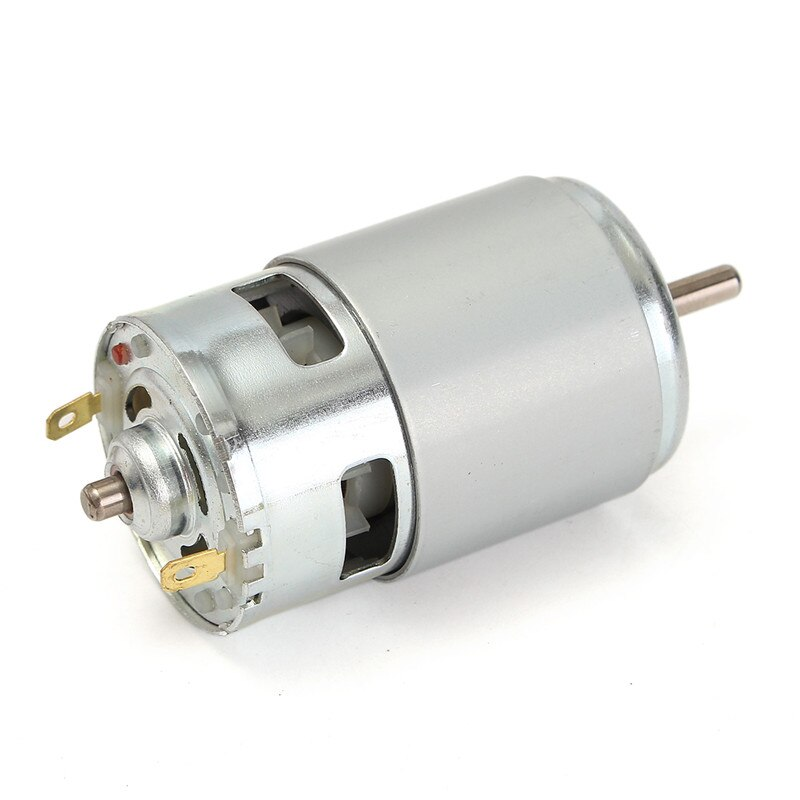
\includegraphics[width=4cm]{gambar/motorDC.jpeg}
	\caption{Jenis-Jenis \emph Joint}
\end{figure}

Motor DC dapat bergerak karena adanya elektromagnet. Saat kumparan diberi arus listrik, permukaan kumparan yang bersifat utara akan bergerak menghadap ke magnet yang berkutub selatan dan kumparan yang bersifat selatan akan bergerak menghadap ke utara magnet. Pada saat ini, kerena kedua kutub saling menyebabkan pergerakan kumparan berhenti. Untuk menggerakannya lagi, tepat pada saat kutub kumparan berhadapan dengan kutub magnet, arah arus pada kumparan dibalik. Dengan demikian, kutub utara kumparan akan berubah menjadi kutub selatan dan kutub selatannya akan berubah menjadi kutub utara.  

Pada saat perubahan kutub tersebut terjadi, kutub selatan kumparan akan berhadapan dengan kutub selatan magnet dan kutub utara kumparan akan berhadapan dengan kutub utara magnet. Karena kutubnya sama, maka akan terjadi tolak menolak sehingga kumparan bergerak memutar hingga utara kumparan berhadapan dengan selatan magnet dan selatan kumparan berhadapan dengan utara magnet. Siklus ini akan berulang-ulang hingga arus listrik pada kumparan diputuskan. Prinsip kerja motor DC dijelaskan pada Gambar 2.13.  
	\begin{figure}[H]
	\centering
	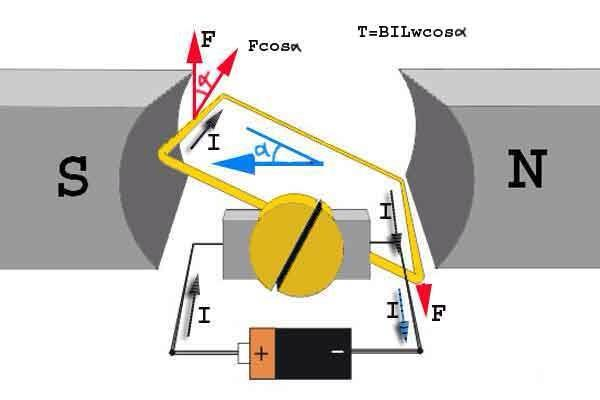
\includegraphics[width=4cm]{gambar/prinsipDC.jpg}
	\caption{Prinsip Kerja Motor DC}
\end{figure}


\section{Regulator}
Dalam suatu rangkaian elektronika dibutuhkan suatu sumber tegangan yang stabil dan sesuai dengan nilai yang dibutuhkan oleh komponen. Untuk memenuhi kebutuhan tersebut digunakanlah sebuah rangkaian regulator. Rangkaian regulator berfungsi untuk mengatur atau menghasilkan nilai tegangan pada nilai tertentu dari suatu tegangan masukan. Regulator dapat mempertahankan nilai tegangan yang keluar tanpa dipengaruhi besar arus yang dikeluarkannya. Regulator tegangan mempunyai banyak jenisnya, salah satunya adalah regulator \textit{switching}.

Regulator \textit{switching} mengatur besarnya nilai tegangan keluaran dengan mensaklar (ON/OFF) tegangan masukan dengan frekuensi berbeda – beda. Kelebihan dari regulator \textit{switching} adalah mempunyai disipasi daya yang terjadi lebih kecil dibandingkan dengan regulator linear. Sedangkan kekurangan yaitu tegangan keluaranya akan berbentuk gelombang akibat adanya proses \textit{switching}. Oleh karena itu, regulator jenis ini umumnya membutuhkan induktor, kapasitor , dan dioda untuk memperhalus tegangan keluaran. Regulator \textit{switching} ada dua jenis yaitu regulator \textit{Buck} dan regulator \textit{Boost}. Regulator \textit{Buck} untuk menghasilkan nilai tegangan keluaran yang lebih kecil dari tegangan masukannya. Sedangkan Regulator \textit{Boost} untuk menghasilkan nilai tegangan yang lebih besar dari tegangan masukannya. Salah satu jenis dari regulator \textit{Buck} adalah LM2596 . Bentuk fisik dari regulator \textit{Buck} ditunjukkan pada Gambar 2.14.

	\begin{figure}[H]
	\centering
	\includegraphics[width=7cm]{gambar/lm2596.jpg}
	\caption{Regulator \textit{Buck} LM2596}
\end{figure}

\section{Arduino}
Arduino  merupakan papan pengembangan dari mikrokontroler yang menggunakan basis Arduino serta menggunakan microchip At 2560. Arduino  memiliki pin input dan output dengan jumlah yang cukup banyak, yaitu sejumlah 54 buah pin input dan output yang 15 diantaranya merupakan pin pulse with modulation (PWM), 16 diantaranya merupakan pin analog input, dan terdapat empat pin yang digunakan sebagai UART (\textit{Serial port hardware}). Arduino ini sudah dilengkapi dengan oscillator sebesar 16Mhz, sebuah port usb, power jack DC, ICSP header serta tombol reset. Gambar 2.15 Merupakan bentuk fisik Arduino.
	\begin{figure}[H]
	\centering
	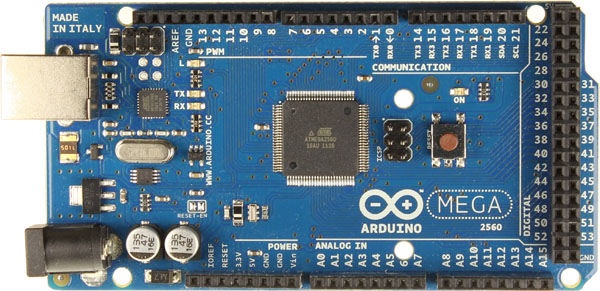
\includegraphics[width=5cm]{gambar/arduino_mega.jpg}
	\caption{Arduino Mega 2560}
	\end{figure}

Arduino Mega 2560 memuat semua yang dibutuhkan untuk mendukung kerja dari sebuah mikrokontroler. Arduino Mega 2560 dapat dengan mudah dioperasikan untuk pengaplikasian ke sebuah sistem kerja karena dapat dihubungkan dengan kabel USB sebagai komunikasinya. Untuk dayanya, Arduino Mega 2560 dapat dihidupkan melalui konektor DC yang dipunyainya dengan diberi tegangan DC, dapat dengan adapter DC atau baterai dengan nilai tegangan sesuai dengan spesifikasi pada Arduino. Spesifikasi Arduino Mega 2560 ditunjukkan pada Tabel 2.1
\begin{table}[H]
	\centering
	\caption{ Spesifikasi Arduino Mega 2560 }
	\resizebox{14cm}{!}{%
		\begin{tabular}{|l|l|}
		\hline
		Mikrokontroler     & Atmega2560$$\hspace{2cm} 		\\ \hline
		Tegangan operasional     & 5 V$$  				\\ \hline
		Tegangan masukan  & 5-12 V$$  		\\ \hline
		Pin digital I/O       & 54 (15 pin untuk keluaran PWM) $$   \\\hline
		Pin analog masukan     & 16$$ 		\\ \hline
		Arus DC per Pin I/O  & 20 mA $$   				\\ \hline
		Arus DC untuk Pin 3.3 V & 50 mA $$  				\\ \hline
		Memori flash    & 256 KB $$ 		\\ \hline
		Kecepatan clock & 16 MHz $$   				\\ \hline
		Dimensi & 101.52 x 53.3 mm $$  				\\ \hline
		
		\end{tabular}%
}
\end{table}

\section{Driver Motor H}
Driver Motor berfungsi sebagai pengontrol dari setiap pergerakan dari motor DC. Pergerakan seperti kecepata, arah putar serta lamanya pergerakan motor DC dapat dikontrol oleh sebuah driver motor. Driver Motor memiliki beberapa jenis tergantung dari spesifikasi dari motor DC yang digunaan. Salah satu jenis driver motor adalah driver motor EMS 30A H-Bridge. Bentuk fisik dari driver motor EMS 30A H-Bride ditunjukkan pada Gambar 2.16.

	\begin{figure}[H]
	\centering
	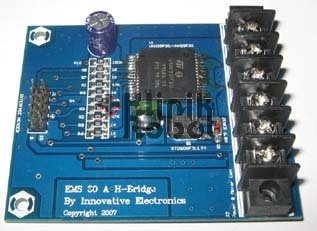
\includegraphics[width=5cm]{gambar/driver_motor.jpg}
	\caption{Driver Motor EMS 30A H-Bridge}
	\end{figure}

Driver Motor EMS 30A H-Bridge merupakan driver motor yang dapat mengoperasikan sebuah Motor DC dengan batasan arus hingga 30 Ampere. Driver ini memiliki 10 buah pin data yang dapat dihubungkan dengan sebuah mikrokontroler. Alokasi pin Driver Motor EMS 30A H-Bridge ini ditunjukkan pada Tabel 2.2.
% Please add the following required packages to your document preamble:
% \usepackage[normalem]{ulem}
% \useunder{\uline}{\ul}{}
\begin{table}[H]
		\centering
	\caption{ Pin pada Driver EMS 30A H-Bridge }
	\resizebox{14cm}{!}{%
	\begin{tabular}{|c|c|c|l|}
		\hline
		Pin  & Nama & I/O & \multicolumn{1}{c|}{Fungsi}                                                                                                                                                 \\ \hline
		1    & MIN1 & I   & Pin input untuk menentukan output MOUT1                                                                                                                                     \\ \hline
		2    & MIN2 & I   & Pin input untuk menentukan output MOUT2                                                                                                                                     \\ \hline
		3    & MEN1 & I/O & \begin{tabular}[c]{@{}l@{}}Pin enable untuk output MOUT1 \\ diberi logika HIGH untuk mengaktifkan half H-Bridge 1, \\ diberi logika LOW untuk menonaktifkannya\end{tabular} \\ \hline
		4    & MEN2 & I/O & \begin{tabular}[c]{@{}l@{}}Pin enable untuk output MOUT2 \\ diberi logika HIGH untuk mengaktifkan half H-Bridge 2, \\ diberi logika LOW untuk menonaktifkannya\end{tabular} \\ \hline
		5    & MSC  & O   & Output tegangan analog yang berbanding lurus dengan arus beban                                                                                                              \\ \hline
		6    & MPWM & I   & Pin input untuk mengatur kerja modul H-Bridge secara PWM                                                                                                                    \\ \hline
		7,9  & VCC  & -   & Terhubung ke catu daya untuk input (5 Volt)                                                                                                                                 \\ \hline
		8,10 & PGND & 0   & Titik referensi untuk caru daya input                                                                                                                                       \\ \hline
	\end{tabular}}
\end{table}

\section{Processing Integrated Development Environment (IDE)}
Processing IDE adalah pemrograman sederhana yang diciptakan untuk pengembangan aplikasi yang berorientasi visual atau pencitraan dengan penekanan pada animasi dan memberi pengguna umpan balik melalui interaksi antarmuka. Para developer Processing IDE ini menginginkan sebuah cara untuk "membuat sketsa" gagasan dalam bentuk kode. Karena pemrograman telah berkembang selama beberapa dekade terakhir. Processing IDE telah mulai digunakan untuk pekerjaan tingkat produksi yang lebih maju. Awalnya dibangun sebagai ekstensi khusus domain Java yang ditargetkan untuk seniman dan desainer, Processing IDE telah berkembang menjadi alat desain dan prototipe lengkap dan penuh yang digunakan untuk pekerjaan instalasi skala besar, grafis gerak, dan visualisasi data yang rumit. Tampilan pada Processing IDE ditunjukkan pada gambar 2.17.
	\begin{figure}[H]
	\centering
	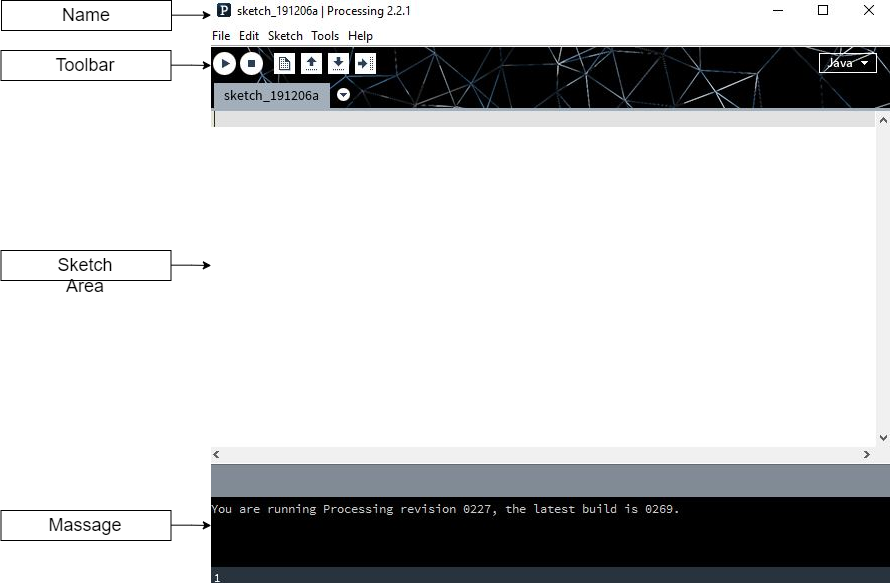
\includegraphics[width=12cm]{gambar/processing_view.png}
	\caption{Processing IDE}
	\end{figure}


\subsection{Syntax dalam Processing IDE }

\subsubsection{Mengatur ukuran}
Ukuran sebuah objek pada processing IDE diatur menggunakan sebuah syntax size() Fungsi size() digunakan untuk menetapkan variabel global lebar dan tinggi dari suatu program. Ukuran untuk panjang dan tinggi tersebut menggunakan ukuran piksel. Lebar diwakili dengan variabel "\textit{width}" dan tinggi diwakili dengan variabel. Untuk objek yang ukurannya tergantung pada layar, selalu gunakan variabel lebar dan tinggi, bukan angka. Ini mencegah masalah saat parameter fungsi size() diubah. Berikut penulisan dari fungsi size() untuk menetapkan lebar dan tinggi suatu program:  size(1000, 1000); 


\subsubsection{Transformasi Bentuk Pada Processing IDE }
Transformasi pada Processing IDE digunakan untuk memindahkan, memutar atau, mengecilkan atau membesarkan suatu objek dan perpindahannya dapat diatur dengan parameter-parameter tertentu di dalam Processing IDE. Transformasi adalah dasar dari pemrograman Processing IDE. Tabel 2.4  adalah adalah contoh penulisan \textit{syntax} dari Transformasi. 

\begin{table}[H]
	\centering
	\caption{ \textit{Syntax} Transformasi}
	\begin{tabular}{|c|l|l|}
		\hline
		No & \multicolumn{1}{c|}{\textit{Syntax}} & \multicolumn{1}{c|}{Keterangan}                                                            \\ \hline
		1  & Translate(x,y)                       & \begin{tabular}[c]{@{}l@{}}x = transisi kiri/kanan \\ y = transisi atas/bawah\end{tabular} \\ \hline
		2  & Rotate(angle)                        & angle=besar sudut rotasi(radian)                                                            \\ \hline
		3  & RotateX(angle)                       & angle=besar sudut rotasi(radian)                                                           \\ \hline
		4  & RotateY(angle)                       & angle=besar sudut rotasi(radian)                                                           \\ \hline
		5  & Rotatez(angle)                       & angle=besar sudut rotasi(radian)                                                           \\ \hline
		6  & Scale(S)                             & s = besar pengecilan pembesaran                                                         \\ \hline
	\end{tabular}
\end{table}
\subsubsection{Shape}
Shape adalah \textit{syntax} pada Processing IDE yang berfungsi untuk membuat berbagai macam bentuk, seperti persegi panjang, lingkaran, garis, dan bentuk lainnya yang dapat diatur ukurannya dengan parameter-parameter tertentu. Tabel 2.3 merupakan contoh dari beberapa \textit{syntax} shape. 
\begin{table}[H]
	\centering
	\caption{\textit{Syntax} Shape}
	\resizebox{14cm}{!}{%
	\begin{tabular}{|l|l|l|l|}
		\hline
		
		No & Sytax                          & Bentuk & Keterangan                                                                                                                                                                                    \\ \hline
		1  & ellipse(a,b,c,d)               &  	\centering 
\includegraphics[width=3cm]{gambar/bulat.png} 
& \begin{tabular}[c]{@{}l@{}}a = koordinatX \\ b = koordinatY \\ c= lebar diameter \\ d= tinggi diameter\end{tabular}                                                                           \\ \hline
		2  & arc(a,b,c,d,start,st op,moode) &  	
\includegraphics[width=3cm]{gambar/busur.png}      & \begin{tabular}[c]{@{}l@{}}a = koordinatX \\ b = koordinatY \\ c = lebar diameter \\ d = tinggi diameter \\ start = sudut mulai \\ stop = sudut akhir \\ mode = PIE, CHORD, OPEN\end{tabular} \\ \hline
		3  & line(x1,y1,x2,y2)              & 	
\includegraphics[width=3cm]{gambar/garis.png}       & \begin{tabular}[c]{@{}l@{}}x1 = koordinatX1 \\ y1 = koordinatY1 \\ x2 = koordinatX2 \\ y2 = koordinatY2\end{tabular}                                                                          \\ \hline
		4  & point(x,y)                     &     	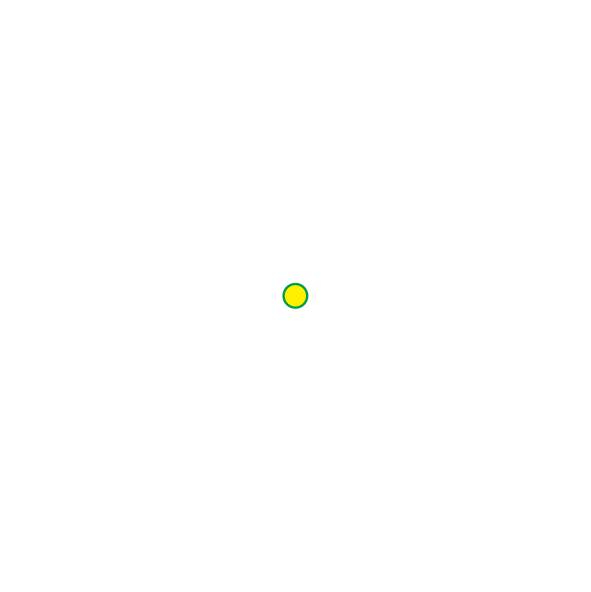
\includegraphics[width=0.5cm]{gambar/point.png}   & \begin{tabular}[c]{@{}l@{}}x = koordinatX \\ y = koordinatY\end{tabular}                                                                                                                      \\ \hline
		5  & rect(a,b,c,d,r)                &    	
\includegraphics[width=3cm]{gambar/kotak.png}    & \begin{tabular}[c]{@{}l@{}}a = koordinatX1 \\ b = koordinatY1 \\ c = koordinatX2 \\ d= koordinatY1\end{tabular}                                                                               \\ \hline
	\end{tabular}}
\end{table}

\subsubsection{Akses Koordinat Mouse }
Processing IDE mempunyai fungsi khusus yaitu dapat melacak posisi mouse baik secara vertical maupun horizontal. Akan tetapi Processing IDE hanya dapat melacak posisi mouse saat sketch dijalankan saja. Nilai default mouseX dan mouseY adalah 0, jadi 0 akan dikembalikan sampai mouse bergerak di depan jendela sketsa. (ini biasanya terjadi saat sketsa dijalankan pertama kali). Setelah mouse bergerak menjauh dari jendela, mouseX akan terus melaporkan posisi terakhirnya. Tabel 2.6  adalah contoh penulisan \textit{syntax} dari mouse. 
\begin{table}[H]
		\centering
	\caption{\textit{Syntax} Koordinat Mouse}
	\begin{tabular}{|c|l|l|}
		\hline
		No & \multicolumn{1}{c|}{\textit{Syntax}} & \multicolumn{1}{c|}{Keterangan}                                                                                                 \\ \hline
		1  & mouseX                               & \begin{tabular}[c]{@{}l@{}}Variabel sistem X memiliki nilai dari \\ koordinat horizontal mouse secara real time\end{tabular}    \\ \hline
		2  & mouseY                               & \begin{tabular}[c]{@{}l@{}}Variabel sistem Y memiliki nilai dari koordinat \\ horizontal mouse secara real time.\end{tabular}   \\ \hline
		3  & mouseButton()                        & \begin{tabular}[c]{@{}l@{}}Bila tombol mouse ditekan, nilai variable sistem \\ disetel ke LEFT,RIGHT, atau CENTER.\end{tabular} \\ \hline
		4  & mouseClicked()                       & \begin{tabular}[c]{@{}l@{}}Dipanggil setelah tombol mouse ditekan \\ dan kemudian dilepaskan.\end{tabular}                      \\ \hline
		5  & mouseDragged()                       & Dipanggil setelah tombol mouse bergerak saat ditekan.                                                                           \\ \hline
	\end{tabular}
\end{table}

\subsubsection{ Compile Sketch }
Program pada Processing IDE dinamakan sketch. Tujuan diberi nama sketch adalah untuk membuat pemrograman bergaya Java ini terasa lebih seperti \textit{scripting}, dan mengadopsi proses \textit{scripting} untuk menulis kode dengan cepat. Sketch disimpan dalam bentuk Sketchbook, folder yang digunakan sebagai default menyimpanan semua proyek Processing IDE. Sketch yang tersimpan dalam Sketchbook dapat diakses dari File - Sketchbook. Sebagai alternatif, File - Open.. dapat digunakan untuk membuka sketch dari tempat lain pada sistem. Gambar 2. 18 adalah opsi toolbar untuk menjalankan sketch. Run (Ctrl + R) adalah opsi untuk menjalankan sketch yang telah dibuat, begitu pula dengan Tweak. Present (Ctrl + Shift + R) berfungsi untuk menjalankan sketch dengan layer penuh (\textit{Fullscreen}). Stop berfungsi untuk menghentikan sketch. 

	\begin{figure}[H]
	\centering
	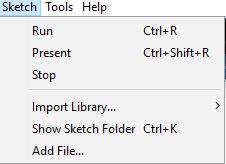
\includegraphics[width=5cm]{gambar/compile.jpg}
	\caption{Toolbar \emph Sketch}
\end{figure}

\subsection{ \textit{Library} untuk Processing IDE }
\subsubsection{ Memuat Huruf (\textit{Font}) pada Processing IDE }
Pfont adalah class yang digunakan untuk penggunaan font pada Processing IDE. Untuk membuat \textit{font} yang akan digunakan dengan Processing IDE, dengan memilih "\textit{Create Font ...}" dari menu \textit{Tools}. Ini akan membuat \textit{font} dalam format Processing IDE yang membutuhkan dan juga menambahkannya ke direktori data sketsa saat ini. Pengolahan menampilkan font menggunakan format font .vlw. Fungsi loadFont() digunakan untuk membuat \textit{font} baru dan textFont () digunakan agar \textit{font} baru yang telah dibuat tersebut aktif. \textit{Syntax} list() berfungsi untuk membuat daftar \textit{font} yang terinstal di komputer, yang merupakan informasi yang berguna untuk digunakan dengan fungsi createFont () untuk mengubah \textit{font} secara dinamis menjadi format yang bisa digunakan di Processing IDE. 


\subsubsection{ Memuat ControlP5 pada Processing IDE }
ControlP5 adalah library yang berfungsi sebagai pengontrol untuk membuat antarmuka dengan user, ControlP5 berupa grafis di dalam sketch Processing IDE yang meliputi Slider, Button, Toggles, Knobs, Radiobutton, dan dapat dengan mudah ditambahkan ke sketch pengolahan. ControlP5 ditulis oleh Andreas Schlegel untuk pemrograman Processing IDE. Library ControlP5 bisa diunduh di laman https://github.com/sojamo/controlp5, atau unduh di library Processing IDE secara langsung. Beberpa contoh dari pengguanaan ControlP5 ditunjukkan pada Gambar 3.2
	\begin{figure}[H]
	\centering
	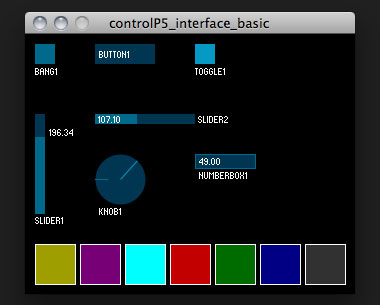
\includegraphics[width=8cm]{gambar/controlp5.jpg}
	\caption{ControlP5}
\end{figure}
Setiap \textit{tools} yang ada pada ControlP5 memiliki fungsi yang berbeda-beda sesuai dengan kegunaannya. ControlP5 dapat dipakai atau saling dikombinasikan agar memudahkan dan memaksimalkan dari GUI yang telah dibuat. ControlP5 nantinya akan bekerja sesuai dengan program yang sudah dimasukkan. Pada Tabel 3.3 merupakan beberapa fungsi dari \textit{tools} yang ada pada ControlP5.
\begin{table}[H]
		\centering
	\caption{Fungsi \textit{Tools} ControlP5}
	\resizebox{14cm}{!}{%
	\begin{tabular}{|c|l|l|l|}
		\hline
		1 & Bang      & Memicu sebuah tindakan ketika ditekan                                                                               & controlP5.addBang("bang1");           \\ \hline
		2 & Button    & Memicu sebuah tindakan ketika sudah dilepas                                                                         & controlP5.addButton("button1");       \\ \hline
		3 & Toggle    & \begin{tabular}[c]{@{}l@{}}Memiliki dua status. \\ TRUE meiliki nilai 1 dan FALSE memiliki nilai 0\end{tabular}     & controlP5.addToggle("toggle1")        \\ \hline
		4 & Slider    & \begin{tabular}[c]{@{}l@{}}Mengatur nilai dengan cara menggeser \\ secara horisontal maupun vertikal\end{tabular}   & controlP5.addSlider("slider2");       \\ \hline
		5 & Knob      & Mengatur sebuah nilai dengan tombol putaran 360°                                                                    & controlP5.addKnob("knob1");           \\ \hline
		6 & NumberBox & \begin{tabular}[c]{@{}l@{}}Kotak yang menampilkan angka dan \\ dapat diubah dengan klik di dalam kotak\end{tabular} & controlP5.addNumberbox("numberbox1"); \\ \hline
	\end{tabular}}
\end{table}


%BAB_3 LAPORAN KP

\chapter{PERANCANGAN SISTEM}
Pada bab ini akan disajikan mekanisme perancangan alat, baik perangkat keras ataupun perangkat lunak untuk mewujudkan sebuah robot lengan. Tahapan perancangan dimulai dari perancangan diagram blok sistem, perancangan perangkat keras, perancangan perangat lunak, perancangan kinematika balik, perancangan GUI, dan integrasi keseluruhan program. 
\section{ Diagram Blok Sistem }
Secara garis besar pada tahapan implementasi dari kinematika pada \textit{arm manipulator robot} SCARA ini menggunakan \textit{output} atau penggerak berupa motor DC dengan \textit{feedback} posisi berupa \textit{potensiometer} sedangkan pada bagian  \textit{input} yang berasal dari GUI yang dibuat pada Processing IDE mengirimkan sebuah koordinat yang digunakan untuk menentukan pergerakan robot berdasarkan fungsi \textit{inverse kinematic}. Gambar \ref{pic.diagram.bloksistem} merupakan diagram blok sistem secara keseluruhan.
\begin{figure}[H]
	\centering
	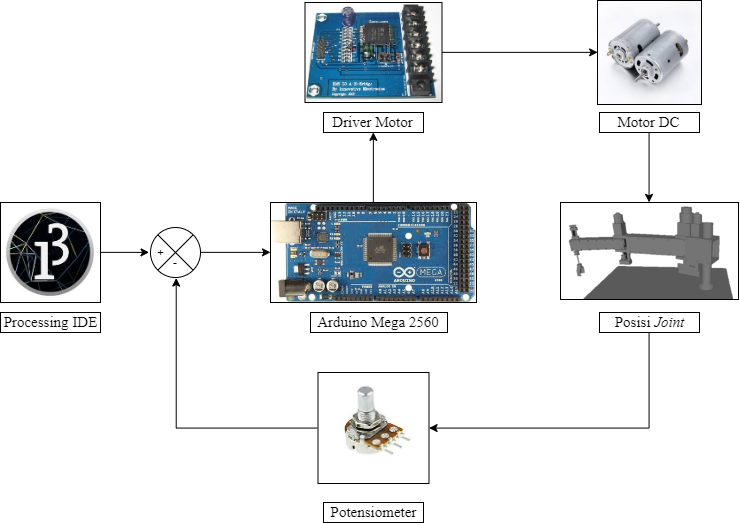
\includegraphics[width=13cm]{gambar/Rangkaian_Diagram.png}
	\caption{Diagram Blok Sistem}
	\label{pic.diagram.bloksistem}
\end{figure}
Pada blok diagram yang disajikan pada Gambar \ref{pic.diagram.bloksistem} sistem terdiri dari bagian – bagian yang meliputi bagian masukan, bagian kendali, bagian keluaran, dan bagian penampil. Pada bagian masukan menggunakan GUI yang dirancang pada Processing IDE yang digunakan sebagai \textit{forward kinematic} serta \textit{inverse kinematic} dimana robot akan bergerak menyesuaikan dengan posisi atau sudut yang diinputkan melauli Processing IDE. 
Pada bagian kontrol menggunakan Arduino Mega 2560 sebagai mikrokontroler yang mengendalikan seluruh operasi dari robot. \textit{Power supply} Arduino sebesar 5 volt DC didapatkan dari regulator tegangan yang menurunkan tegangan dari 24 volt DC ke 5 volt DC. 

Pada bagian keluaran, pin \textit{Pulse With Modulation} (PWM) pada Arduino Mega 2560 dihubungkan dengan \textit{driver} motor yang digunakan untuk mengontrol arah pergerakan dari motor DC serta kecepatan pergerakan dari motor DC. Pergerakan arah putaran motor DC bergantung pada \textit{feedback} posisi setiap sendi yang diberikan oleh \textit{potensiometer}. Tiga buah pin digital ardunio dihubungkan pada rangkaian \textit{switch} yang menggunakan IC TIP31 yang berfungsi sebagai kontrol dari \textit{End-Effector} yang dioperasikan menggunakan tekanan udara yang dikontrol oleh \textit{valve pneumatic.}

Pada bagian penampil merupakan bentuk dari rancangan GUI yang dirancang dalam Processing IDE melalui sebuah bentuk pemrograman. Dalam tampilan GUI terdapat beberapa \textit{tools} yang dapat untuk mengatur pergerakan robot SCARA. Pada GUI menampilkan nilai dari sudut, dan posisi serta animasi robot SCARA pada kondisi langsung dari pergerakan robot SCARA.
\section{ Perancangan Perangkat Keras }
Perancangan perangkat keras pada \textit{arm manipulator robot} SCARA terdiri dari dua bagian yaitu bagian mekanis dan elektronis. Bagian  mekanis merupakan bagian \textit{hardware} yang meliputi desain, bahan dan bentuk dari\textit{ arm manipulator robot} SCARA. Bagian elektronis merupakan bagian \textit{hardware} yang meliputi sistem – sistem yang berkaitan dengan rangkaian pada robot SCARA seperti rangkaian pada desain \textit{board} serta komponen – komponen elektronis pendukung.
\subsection{ Sistem Mekanis }
Sistem mekanika dari robot lengan bergantung dari konfigurasi robot lengan. Konfigurasi robot lengan terbagi menjadi enam, yaitu konfigurasi \textit{Articulated}, konfigurasi SCARA, konfigurasi \textit{Spherical}, konfigurasi \textit{Cylindrical}, dan konfigurasi \textit{Cartesian}. Pada Kerja Praktik ini konfigurasi robot lengan yang digunakan adalah konfigurasi SCARA dengan dua \textit{joint} \textit{revolute} dan satu \textit{end-effector}. Sistem mekanik dari lengan robot tiga DOF sangat berpengaruh dan mendominasi sistem karena bentuk dan pergerakan dari mekanik akan mempengaruhi elektronis serta program. Sistem mekanik yang baik sangat mendukung dari pergerakan robot, oleh karena itu perancangan mekanik harus proporsional dari panjang setiap lengan, lebar serta tinggi robot. Gambar \ref{pic.freebodyscara} merupakan \textit{free body} dari robot SCARA. Gambar \ref{pic.fisikscara} merupakan bentuk fisik dari robot SCARA yang digunakan pada penelitian kali ini.
\begin{figure}[H]
	\centering
	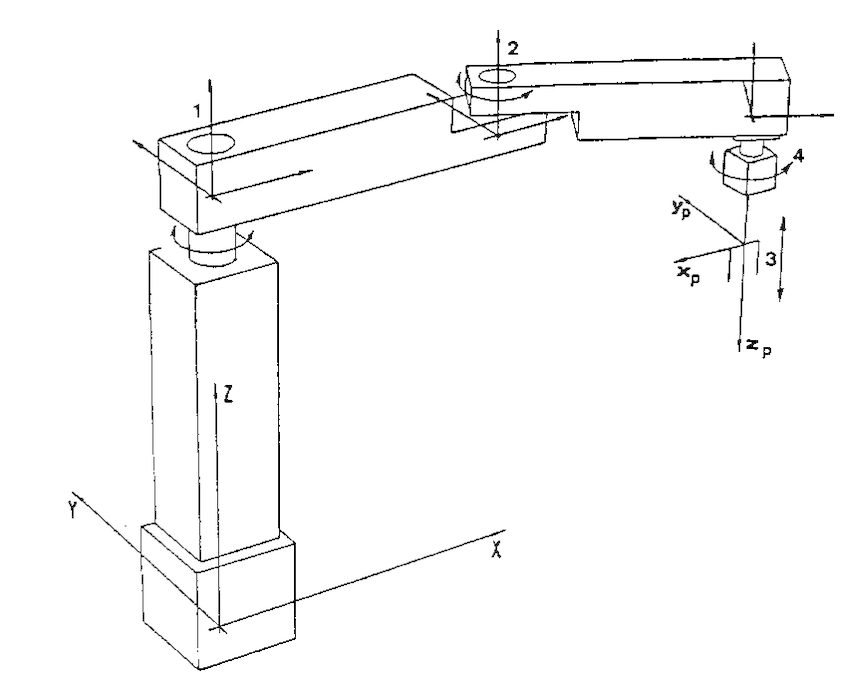
\includegraphics[width=7cm]{gambar/scaraa.png}
	\caption{\textit{Free Body} Robot SCARA}
	\label{pic.freebodyscara}
\end{figure}
\begin{figure}[H]
	\centering
	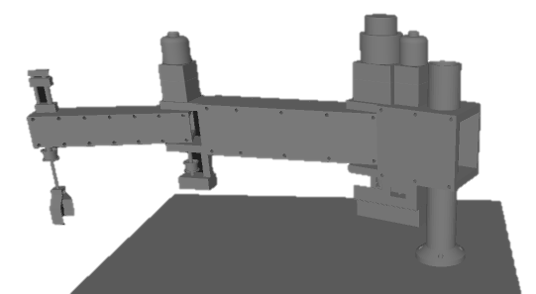
\includegraphics[width=7cm]{gambar/3dscara.png}
	\caption{Bentuk Fisik Robot SCARA}
	\label{pic.fisikscara}
\end{figure}
Robot SCARA merupakan robot yang meiliki tiga buah derajar kebebasan (DOF) yang terletak pada \textit{shoulder}, \textit{elbow}, dan pada \textit{end-effector}. Seluruh derajat kebebasan menggunakan sebuah motor DC yang didalamnya terdapat\textit{ gear box} untuk motor DC yang ada pada \textit{shoulder} dan \textit{elbow} untuk melakukan pergerakan. Sedangkan motor DC pada \textit{end-effector} dibantu oleh sebuah \textit{belt} untuk menyalurkan putaran dari motor yang terletak pada \textit{shoulder}. Pergerakan pada masing-masing \textit{joint} memiliki jangkauan maksimum yang berbeda-beda. Jangkauan juga dipengaruhi oleh panjangnya lengan yang dimiliki oleh robot SCARA tersebut. Tabel \ref{tbl.spesifikasiscara} merupakan spesifikasi dari robot SCARA yang digunakan.


\begin{table}[H]
	\centering
	\caption{Spesifikasi Robot SCARA}
	\label{tbl.spesifikasiscara}
		\begin{tabular}{|l|l|}
			\hline
			Main arm length      & 360 mm		\\ \hline
			Fore arm length      & 290 mm  				\\ \hline
			Shoulder movement    & 180 °  		\\ \hline
			Elbow movement       & 200 °   		\\ \hline
			Wrist rotation       & 360 ° 		\\ \hline
			Up \& down movement  & 150 mm   				\\ \hline
			Maximum tip velocity & 3.0 kg  				\\ \hline
		\end{tabular} 
	\end{table}
Desain pada\textit{ arm manipulator robot} SCARA berbahan besi dengan tebal 2 mm dengan tiga derajat kebebasan yang meliputi bagian \textit{shoulder}, \textit{elbow} serta \textit{end-effector}. Desain robot SCARA terbagi menjadi dua bagian. Bagian utama adalah \textit{box} panel yang berisi sistem elektronis utama dan pada bagian yang lain merupakan lengan dari robot SCARA sendiri. Terdapat juga tiga buah saluran udara yang berfungsi untuk mentransformasikan tekanan udara untuk pergerakan vertikal dari \textit{end-effector} yang berasal dari sebuah kompresor.  Dalam komunikasinya dengan komputer personal, robot SCARA dihubungkan dengan konektor USB. Gambar \ref{pic.boxpanel} merupakan bentuk fisik dari box panel pada Robot SCARA.
\begin{figure}[H]
	\centering
	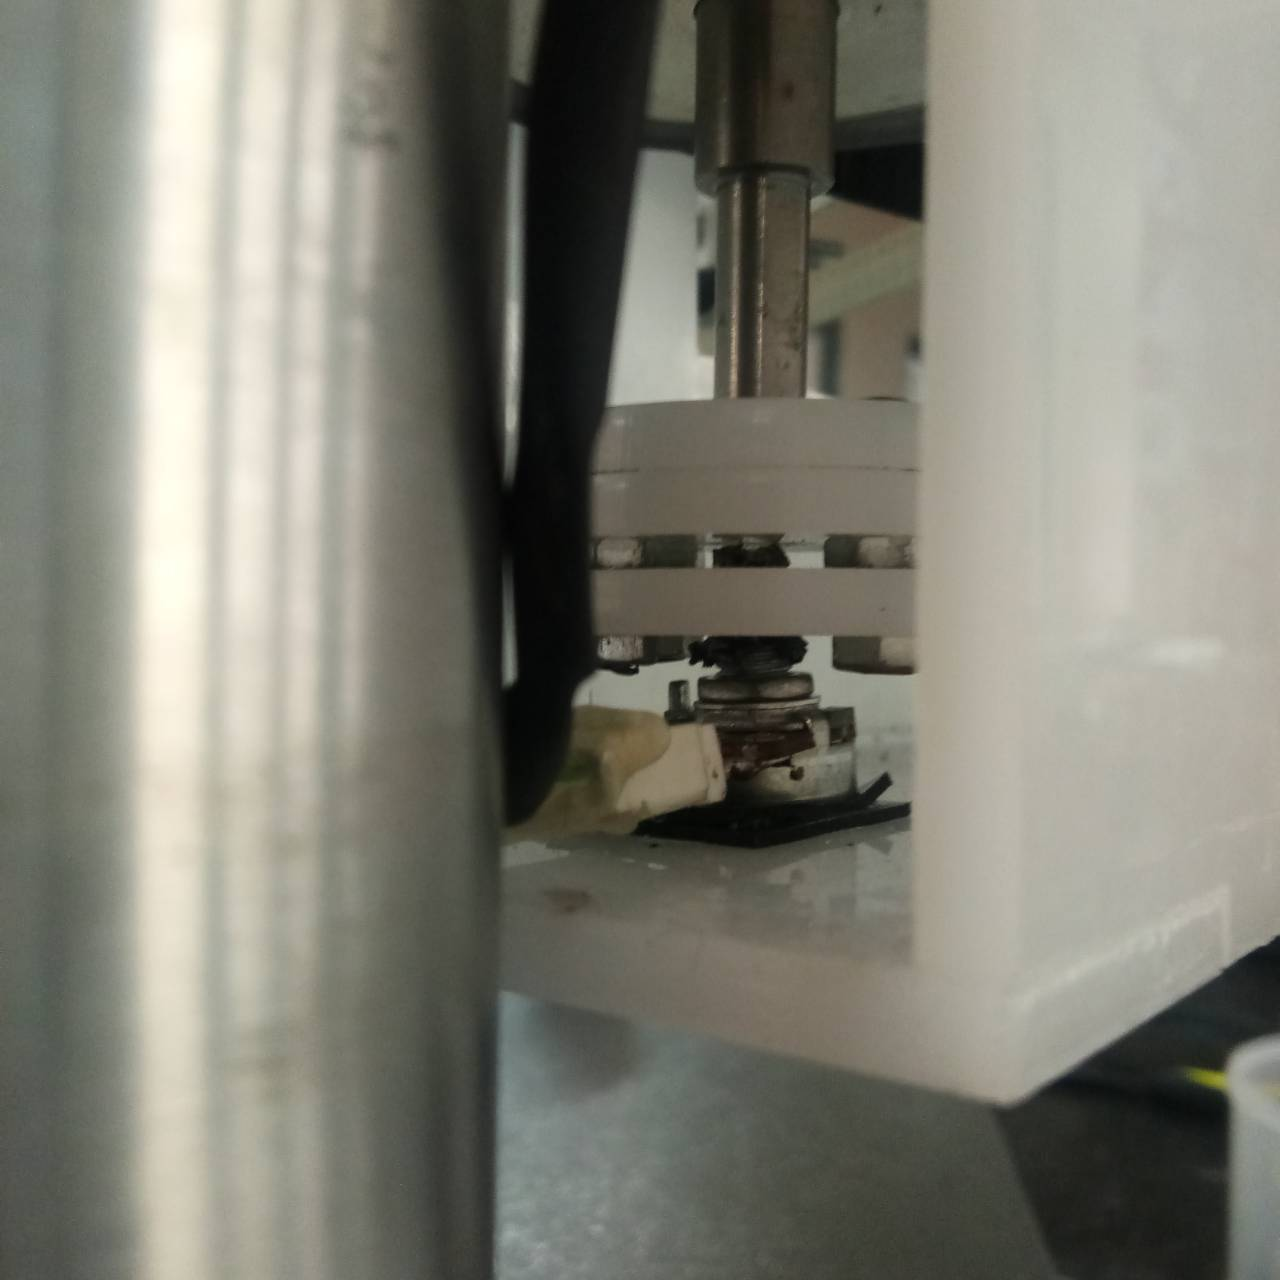
\includegraphics[width=5cm]{gambar/potsementara.jpg}
	\caption{Box Panel Robot SCARA}
	\label{pic.boxpanel}
\end{figure}

Pada \textit{arm manipulator robot} SCARA menggunakan penggerak berupa motor DC 12 Volt dengan \textit{gearbox} sehingga mampu mengangkat beban berat karena torsi pada motor bertambah besar. Motor DC dikontrol oleh \textit{Driver} Motor EMS 30A H-\textit{Bridge} melalui mikrokontroler Arduino Mega 2560. Tabel \ref{tbl.spesifikasimotordc} merupakan spesifikasi dari motor DC yang digunakan pada robot SCARA. 

	\begin{table}[H]
	\centering
	\caption{Spesifikasi Motor DC pada Robot SCARA}
	\label{tbl.spesifikasimotordc}
	\resizebox{15cm}{!}{%
		\begin{tabular}{|l|l|}
			\hline
			Moments of inertia of the main arm ($J_{1}$)    							& $0.0980kgm^{2}$ 				\\ \hline
			Moments of inertia of the fore arm ($J_{2}$)    							& $0.0115 kgm^{2}$ 				\\ \hline
			Masses of the main arm	($m_{1}$)											& $1.90kg$   					\\ \hline
			Masses of the fore arm  ($m_{2}$)     										& $0.93kg$   					\\ \hline
			Motor and equivalent inertias ($J_{m}$)      								& $3.3*10^{-6}kgm^{2}$ 			\\ \hline
			Back emf constants for main arm and fore arm motor ($K_{e1}=K_{e2}$)  		& $0.047Nm/A$   				\\ \hline
			Armature resistance for main arm and fore arm motor($R_{a1}=R_{a2}$)		& $3.5\Omega$  					\\ \hline
			Armatures inductances for main and fore arm motor  ($L_{a1}=L_{a2}$) 		& $1.3mH$ 						\\ \hline
		\end{tabular}%
	}
\end{table}
%%
Pada bagian \textit{gearbox} pada masing-masing motor DC terdapat \textit{potensiometer} sebagai sensor posisi. \textit{Potensiometer} ditempatkan pada bawah motor DC yang terhubung langsung. Setiap pergerakan dari motor DC, \textit{potensiometer} secara otomatis ikut bergerak dan kemudian mengirimkan nilai data analog ke Arduino Mega. Data yang berhasil diterima oleh Arduino Mega 2560 kemudian diolah dan mendapatkan hasil berupa besar sudut pada pergerakan \textit{joint} tersebut. Gambar \ref{pic.potensiometer} merupakan bentuk fisik dari motor DC serta pemasangan \textit{potensiometer}.
\begin{figure}[H]
	\centering
	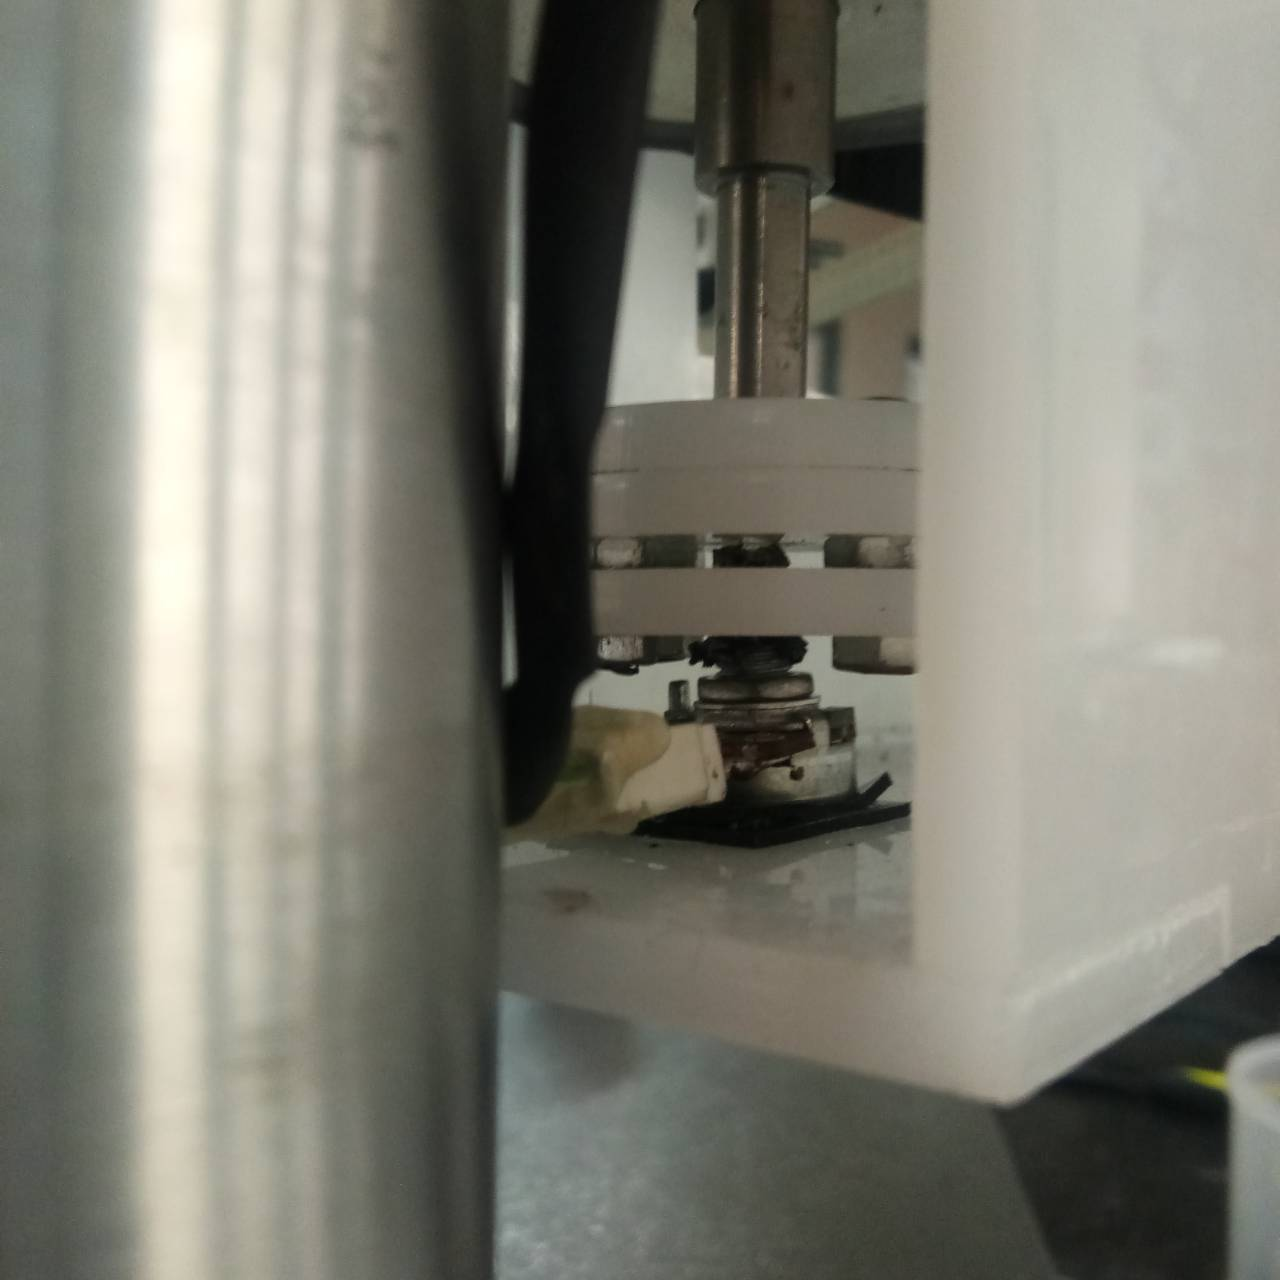
\includegraphics[width=5cm]{gambar/potsementara.jpg}
	\caption{Motor DC dengan \textit{Potensiometer}}
	\label{pic.potensiometer}
\end{figure}

Pada bagian \textit{end-effetor} menggunakan pergerakan translasi. Pergerakan translasi pada robot \textit{end-effector} merupakan gerak translasi pada sumbu Y. Pada robot SCARA pergerakan ini ada pada bagian \textit{end-effector} yang bergerak secara vertikal atau naik turun. Dengan pergerakan ini posisi \textit{end-effector} mengalami perubahan pada posisi tingginya. Pergerakan translasi juga terdapat pada bagian \textit{end-effector} yang menyebabkan sebuah \textit{gripper }\textit{ end-effector} dapat membuka dan menutup karena sebuah sistem mekanik yang telah ada di dalamnya. Selain dari pergerakan translasi, pergerakan pada end-effector juga terdapat rotasi. Pergerakan ini dilakukan oleh satu buah motor DC yang ditempatkan pada bagian \textit{shoulder} dengan dihubungkan melalui sebuauh \textit{belt}. Pengoperasian pada motor DC ini juga dilakukan oleh \textit{Driver} Motor EMS 30A H-\textit{Bridge}. Gambar \ref{pic.endeffectorfisik} merupakan bentuk fisik dari \textit{end-effector} pada robot SCARA yang digunakan. 
\begin{figure}[H]
	\centering
	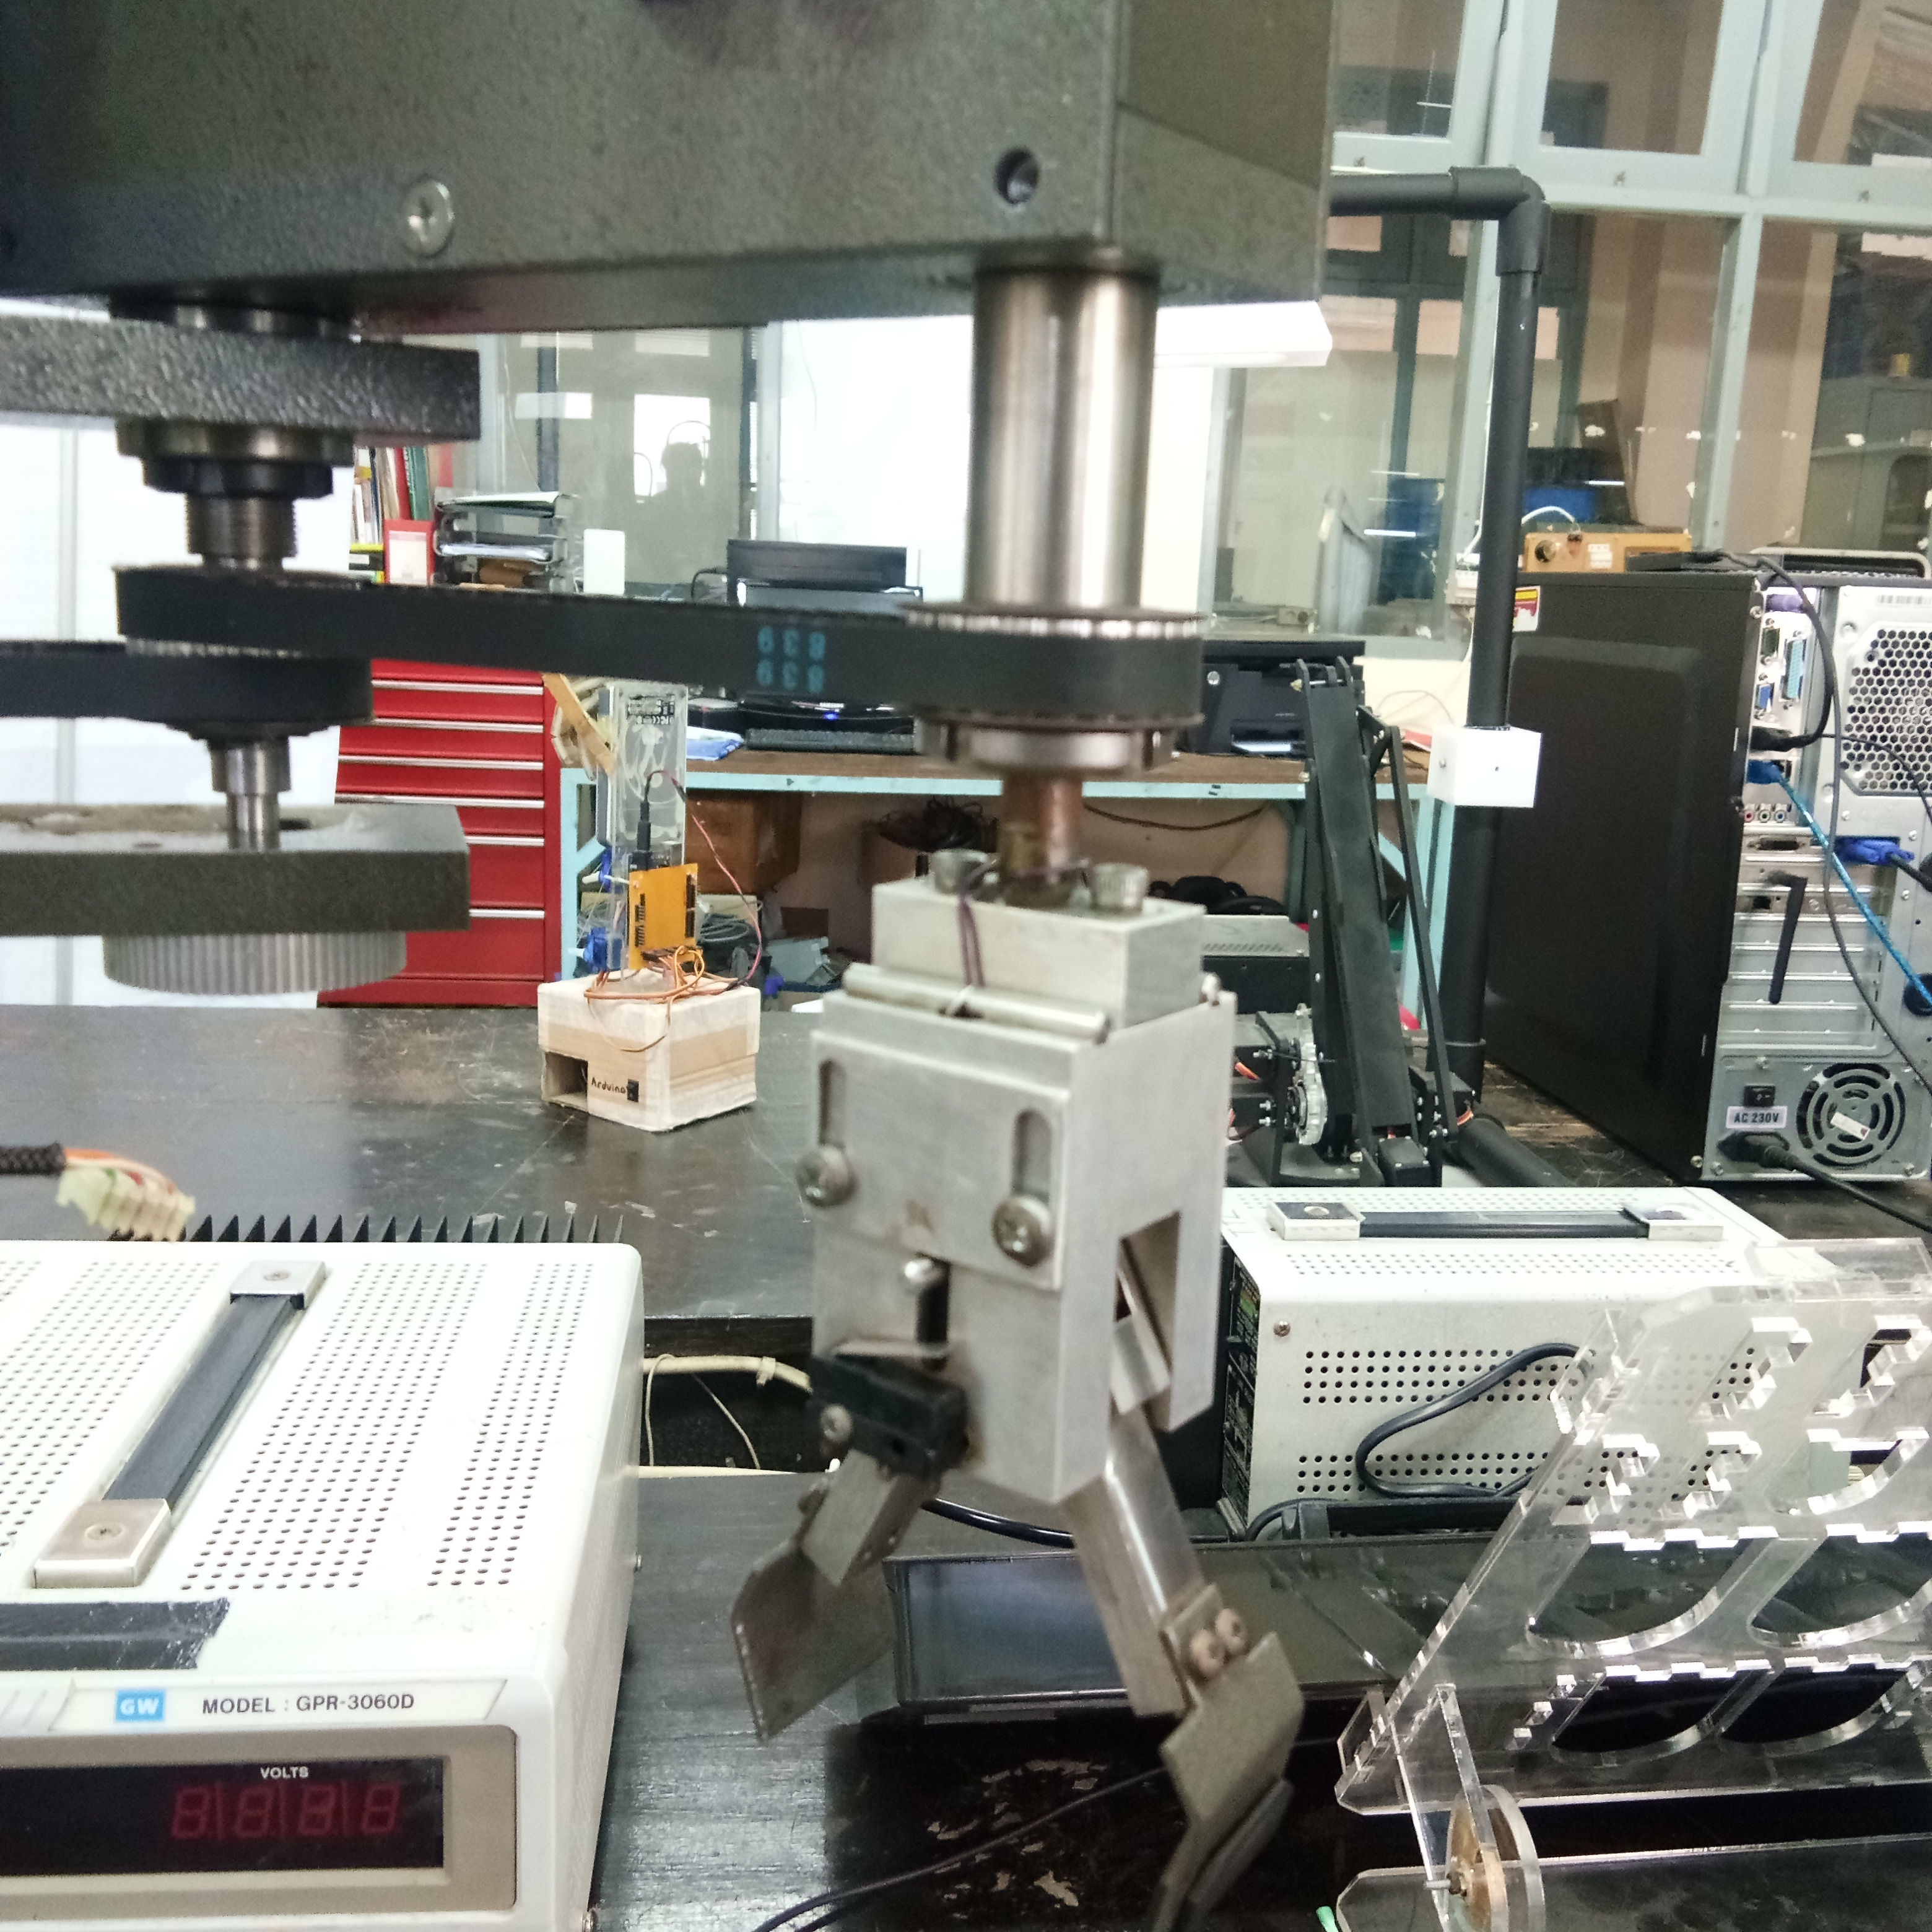
\includegraphics[width=5cm]{gambar/capitsementara.jpg}
	\caption{\textit{End-Effector} Robot SCARA}
	\label{pic.endeffectorfisik}
	
\end{figure}
Semua pergerakan pada \textit{end-effector} ditenagai oleh sebuah tekanan udara yang bersumber dari sebuah kompresor. Tekanan udara diaplikasikan pada sebuah \textit{pneumatic} dengan sistem kerja translasi yang dapat menyebabkan sebuah objek dapat bergerak pada sebuah garis lurus. Gambar \ref{pic.pneumatic} merupakan bentuk fisik dari \textit{pneumatic} yang digunakan pada robot SCARA. 
\begin{figure}[H]
	\centering
	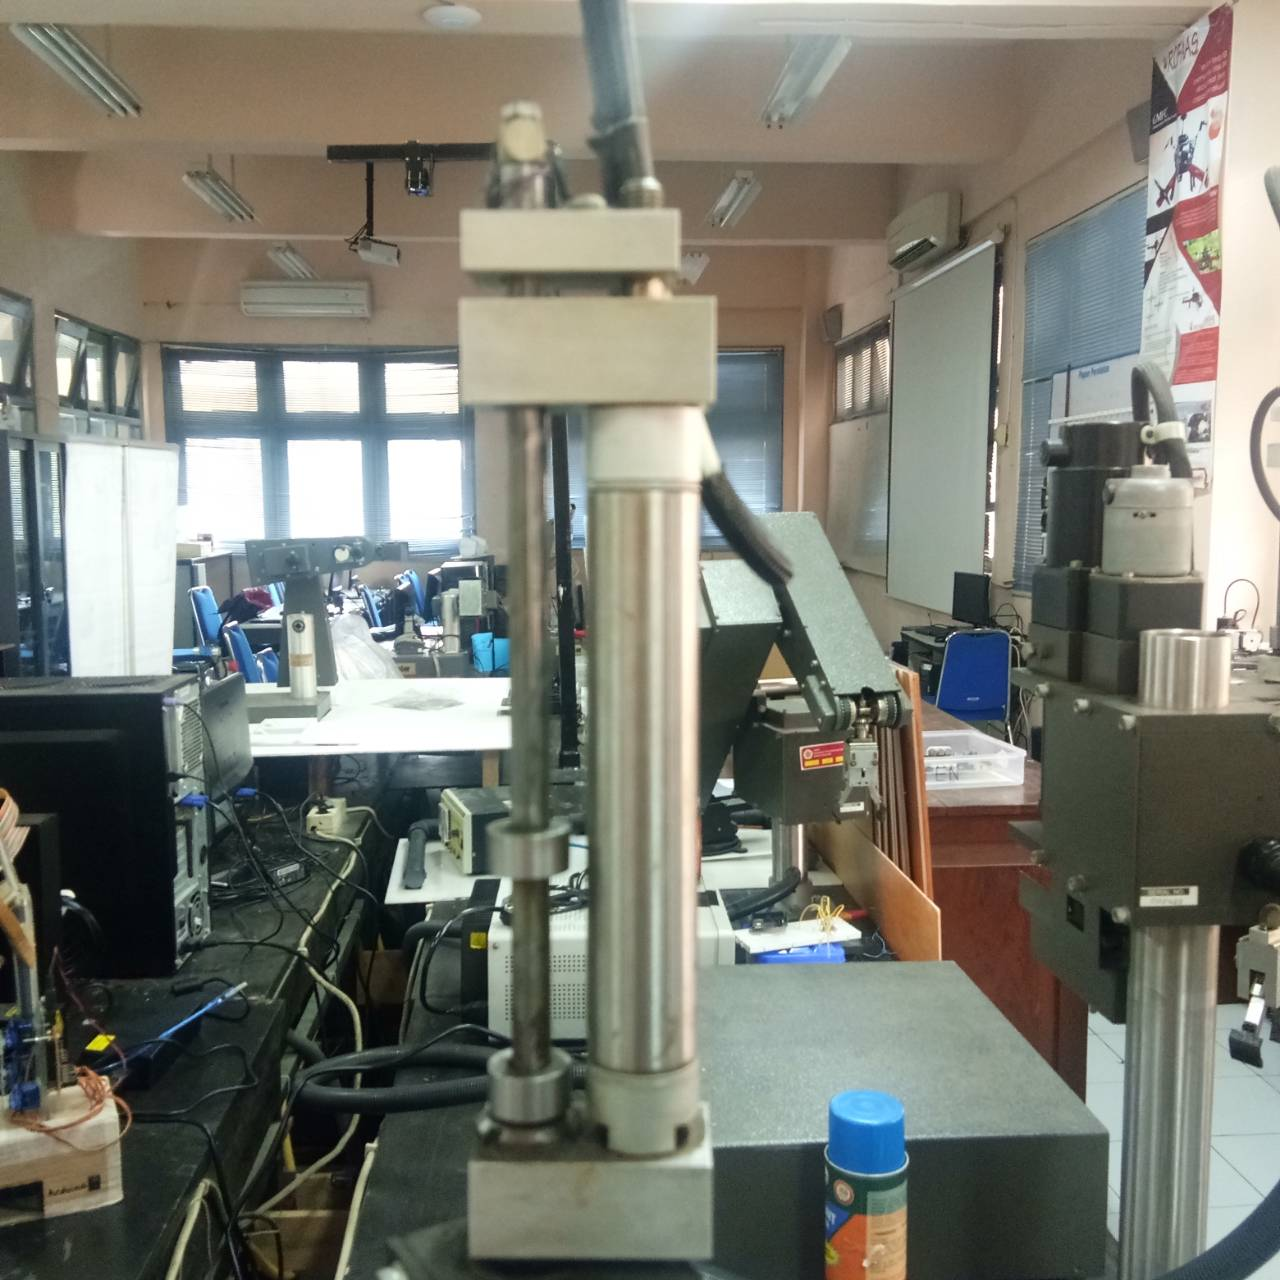
\includegraphics[height=6cm]{gambar/penuamticsementara.jpg}
	\caption{Bentuk Fisik \textit{Pneumatic}}
	\label{pic.pneumatic}
\end{figure}
Kompresor yang digunakan untuk menghasilkan sebuah tekanan udara merupakan sebuah kompresor listrik dengan kapasitas 8 bar. Kompresor ini dioperasikan menggunakan sumber tegangan AC 220 Volt. Ketika kapasitas udara sudah terpenuhi kompresor ini dapat digunakan tanpa menggunakan sumber tegangan tetapi hanya sebatas kapasitas udara yang disimpan. Gambar \ref{pic.kompresor} merupakan bentuk fisik dari kompresor yang digunakan.
\begin{figure}[H]
	\centering
	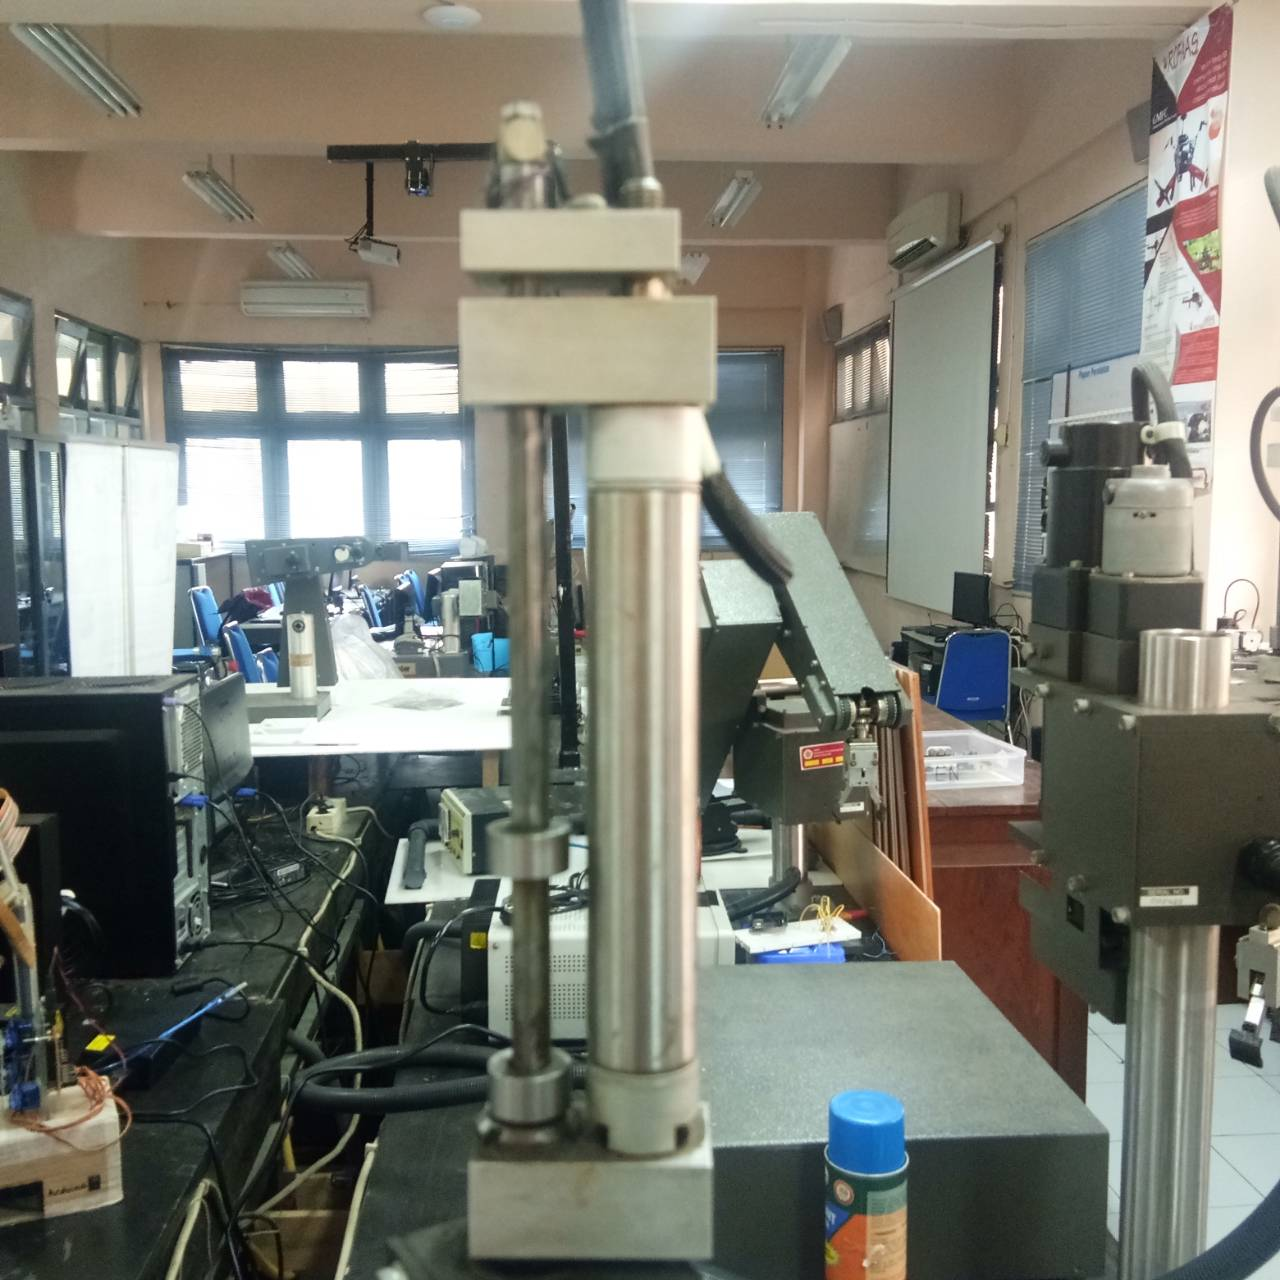
\includegraphics[height=6cm]{gambar/penuamticsementara.jpg}
	\caption{Bentuk Fisik Kompresor}
	\label{pic.kompresor}
\end{figure}

Rancangan robot secara keseluruhan ditampilan pada Gambar \ref{pic.scarasamping} yang merupakan rancangan tampak samping, Gambar \ref{pic.scaraatas} merupakan rancangan tampak atas dan Gambar \ref{pic.scaradimensi} merupakan rancangan dimensi robot. 
\begin{figure}[H]
	\centering
	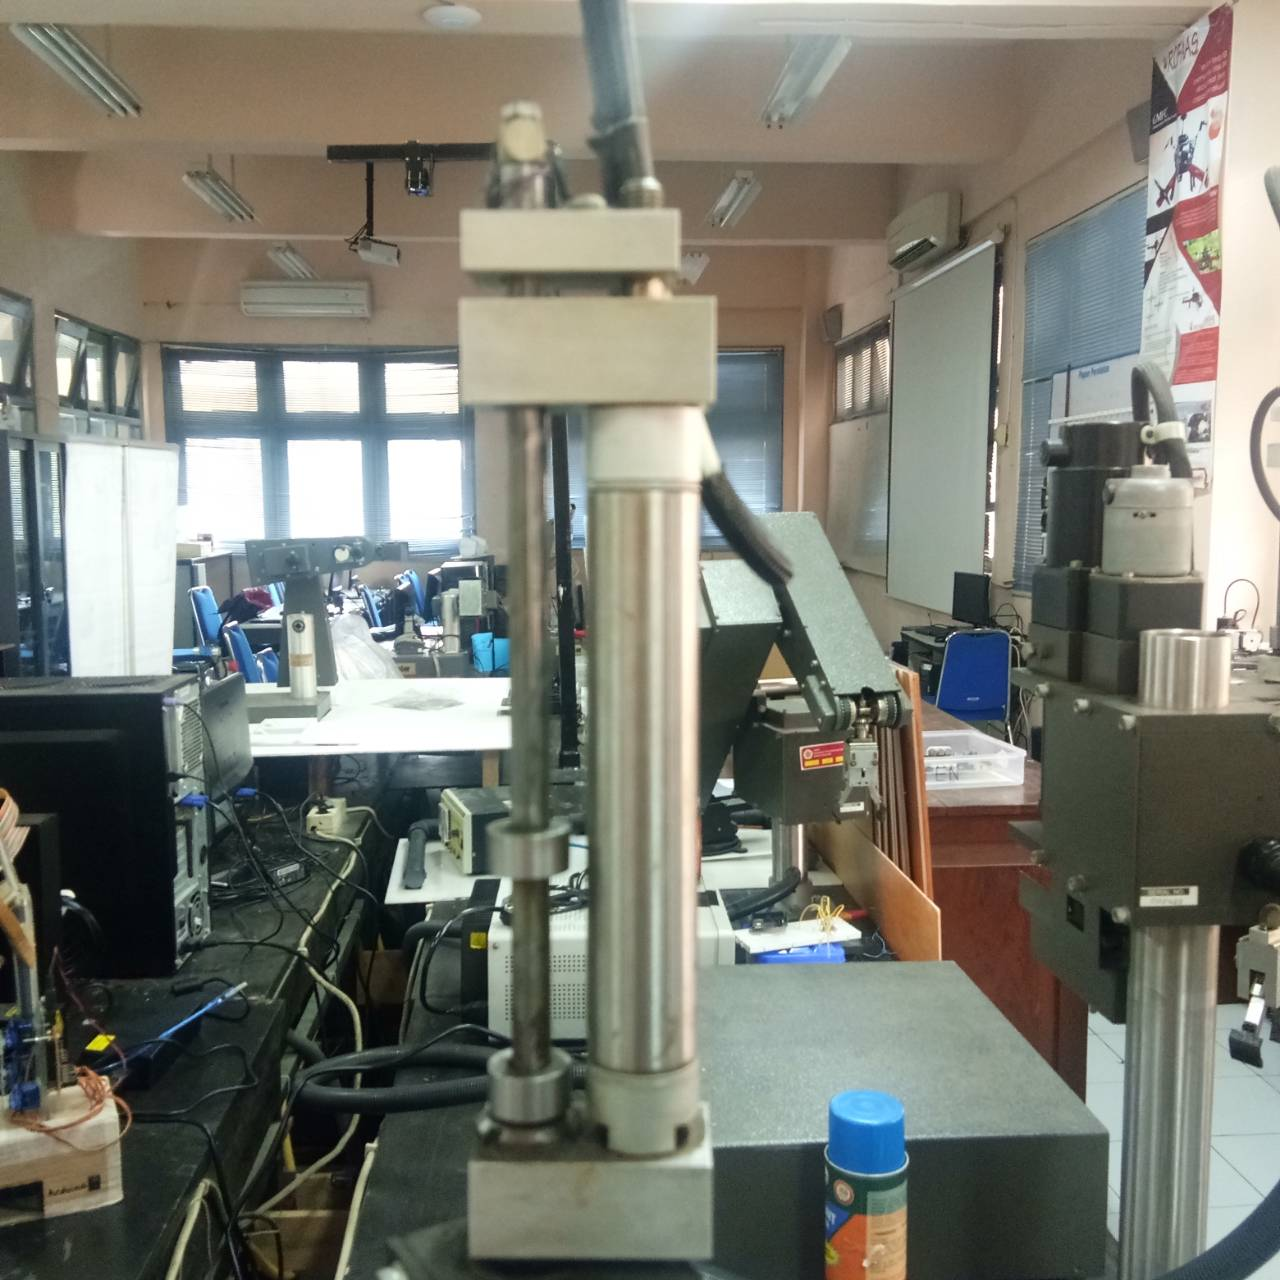
\includegraphics[height=6cm]{gambar/penuamticsementara.jpg}
	\caption{Rancangan Tampak Samping}
	\label{pic.scarasamping}
\end{figure}

\begin{figure}[H]
	\centering
	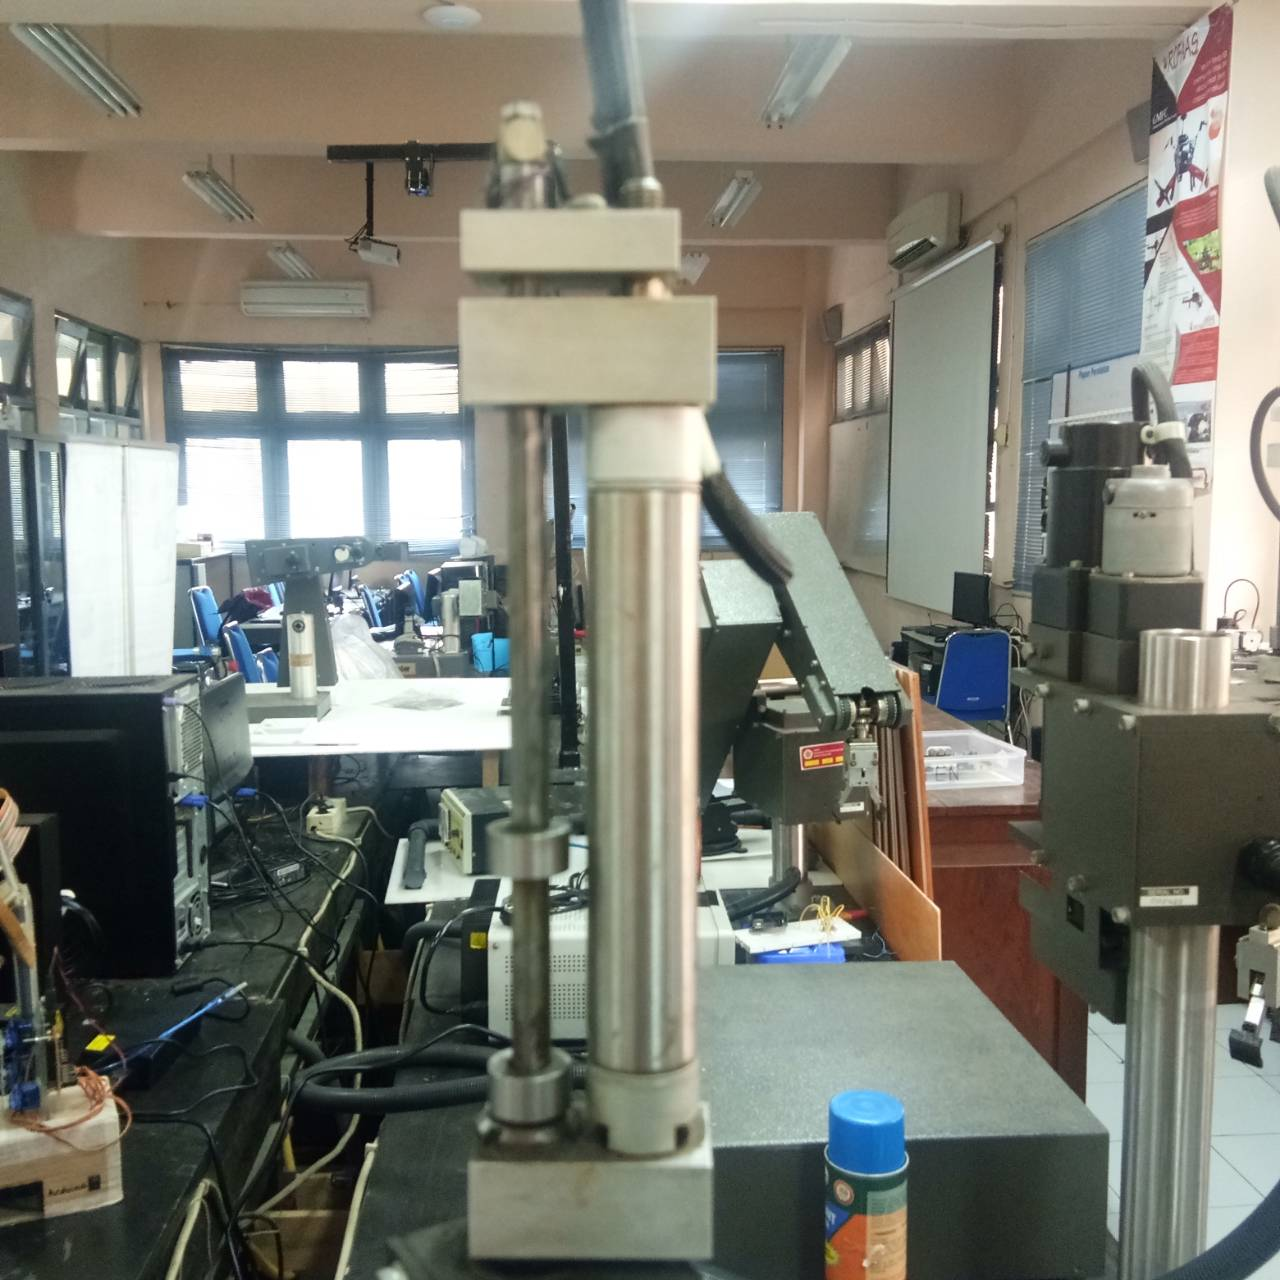
\includegraphics[height=6cm]{gambar/penuamticsementara.jpg}
	\caption{Rancangan Tampak Atas}
	\label{pic.scaraatas}
\end{figure}

\begin{figure}[H]
	\centering
	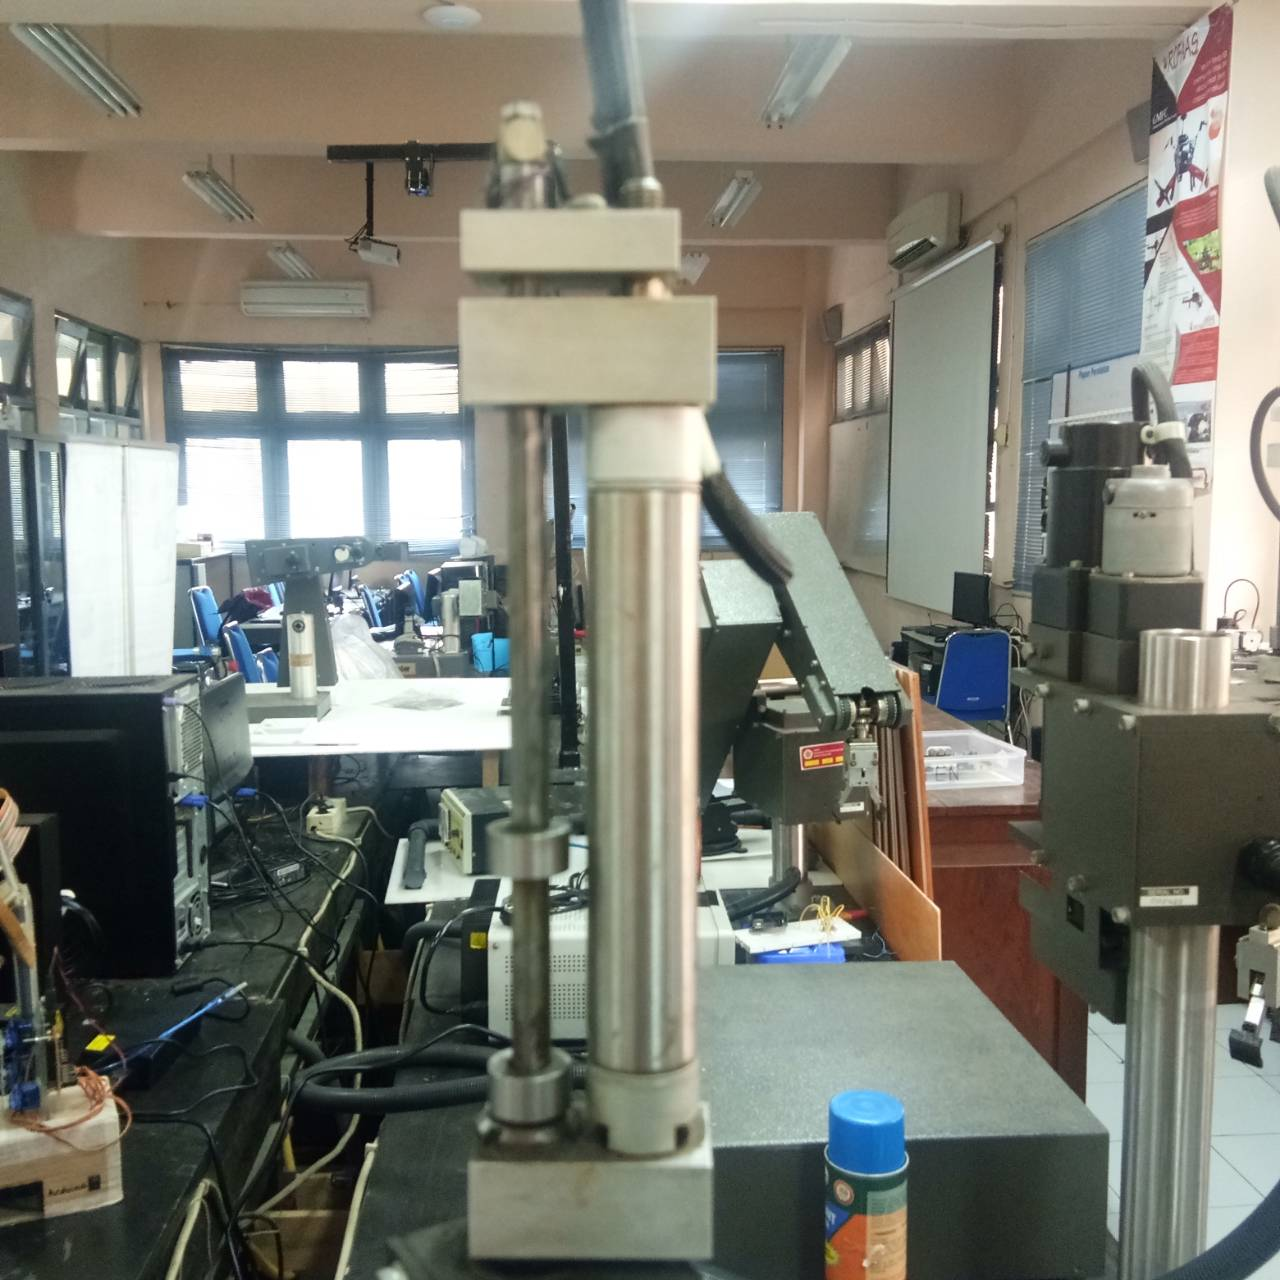
\includegraphics[height=6cm]{gambar/penuamticsementara.jpg}
	\caption{Dimensi Robot}
	\label{pic.scaradimensi}
\end{figure}

\subsection{Rangkaian Elektronika}
\subsubsection{Rangkaian Motor DC}
Rancangan kendali pada \textit{arm manipulator robot} SCARA ini menggunakan tiga buah motor DC dengan masing – masing dilengkapi dengan \textit{gearbox} untuk memperkuat torsi yang dihasilkan oleh motor DC. Pada  \textit{gearbox} masing – masing motor  DC diberikan sensor \textit{potensiometer} sebagai \textit{feedback} untuk memberikan posisi motor DC pada keseluruhan sistem. Motor DC diletakkan pada \textit{shoulder} untuk \textit{end-effector} satu buah yang dihubungkan melalui \textit{belt}, pada \textit{shoulder} satu buah, dan pada \textit{elbow} satu buah. Ketiga motor DC tersebut masing-masing menggunakan \textit{Driver} Motor EMS 30A H-\textit{Bridge} dalam sistem kerjanya. Pada masing – masing motor DC membutuhkan catu daya 12 Volt DC. Rangkaian \textit{driver} motor mendapat sumber tegangan DC 12V untuk disalurkan ke pada motor DC dan 5 Volt untuk kerja dari driver motor sendiri. 12 Volt didapat dari tegangan keluaran yang dihasilkan oleh regulator \textit{Buck} yang berseumber dari tegangan DC 24 Volt setelah dilakukan \textit{converter} AC to DC. Ragkaian utama \textit{Driver} Motor EMS 30A H-\textit{Bridge} ditunjukkan pada Gambar \ref{pic.drivermotor} dan pada Gambar \ref{pic.motordcdriver} merupakan rangkaian antara motor DC, driver motor, dan Arduino Mega.  
\begin{figure}[H]
	\centering
	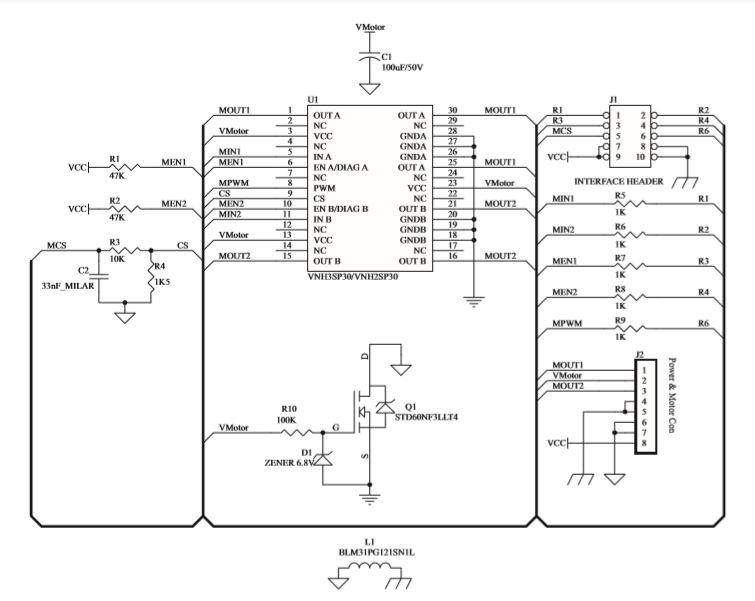
\includegraphics[width=10cm]{gambar/rangakaiandriver.jpg}
	\caption{Rangkaian Utama \textit{Driver} Motor EMS 30A H-\textit{Bridge}}
	\label{pic.drivermotor}
\end{figure}
\begin{figure}[H]
	\centering
	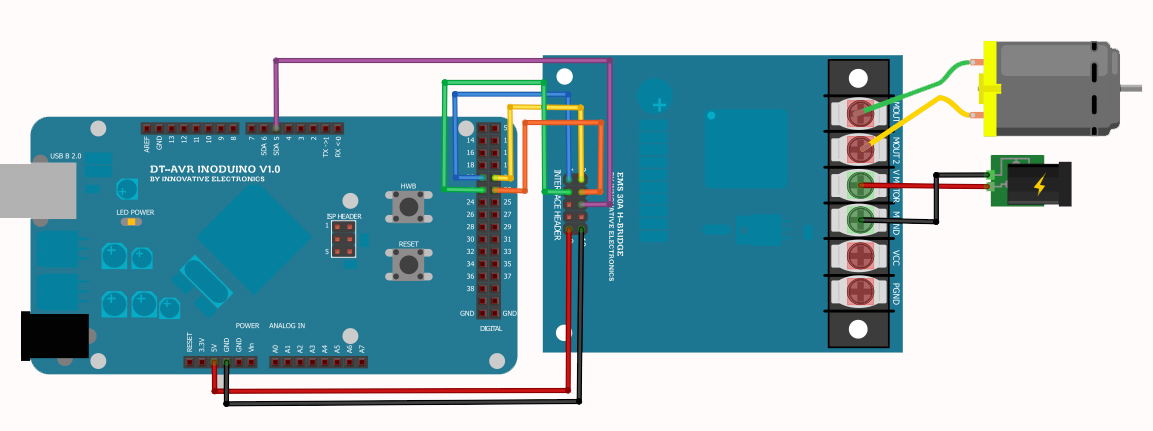
\includegraphics[width=10cm]{gambar/drivermotor.jpg}
	\caption{Rangkaian Arduino antara \textit{Driver} Motor dan Motor DC}
	\label{pic.motordcdriver}
\end{figure}
\subsubsection{Rangkaian \textit{Valve Pneumatic}}
\textit{End-Effector} menggunakan tekanan udara dalam melakukan pergerakannya. Tekanan udara ini dikontrol menggunakan sebuah\textit{valve relay}. \textit{Valve relay} yang digunakan dapat mengkontrol tekanan udara hingga delapan bar. \textit{Valve relay} dapat bekerja pada tegangan DC 24 Volt. Tegangan 24 Volt pada \textit{valve relay} didapat dari keluaran dari rangkaian AC-DC yang dilakukan oleh dioda \textit{bridge} dengan masukan awalnya adalah tegangan AC 24 Volt yang diberikan oleh sebuah tranformator. Dengan besaran tegangan 24 Volt maka sebuah arduino tidak dapat mengkontrolnya. Oleh karena itu, diberi sebuah rangkaian pembantu yang prinsipinya bekerja seperti saklar. Rangkaian tersebut diotaki oleh IC TIP31 yang nantinya akan menerima sinyal data digital dari Arduino Mega 2560 dan akan membuka jalur untuk tegangan 24 Volt. Gambar \ref{pic.fisikvalve} merupakan bentuk fisik dari \textit{valve relay} yang digunaakan dan Gambar \ref{pic.skematikvalve} merupakan rangkaian dari \textit{valve pneuamtic} dengan rangkaian TIP31.
\begin{figure}[H]
	\centering
	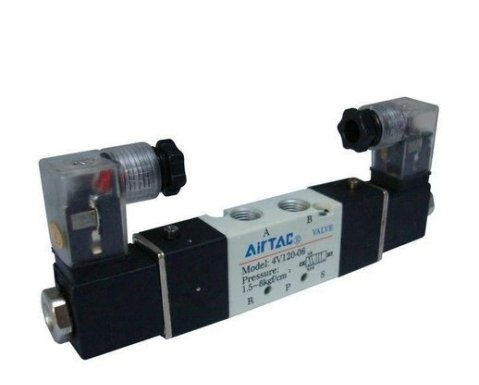
\includegraphics[width=5cm]{gambar/relay.jpg}
	\caption{Bentuk Fisik dari \textit{Valve Pneumatic}}
	\label{pic.fisikvalve}
\end{figure}
\begin{figure}[H]
	\centering
	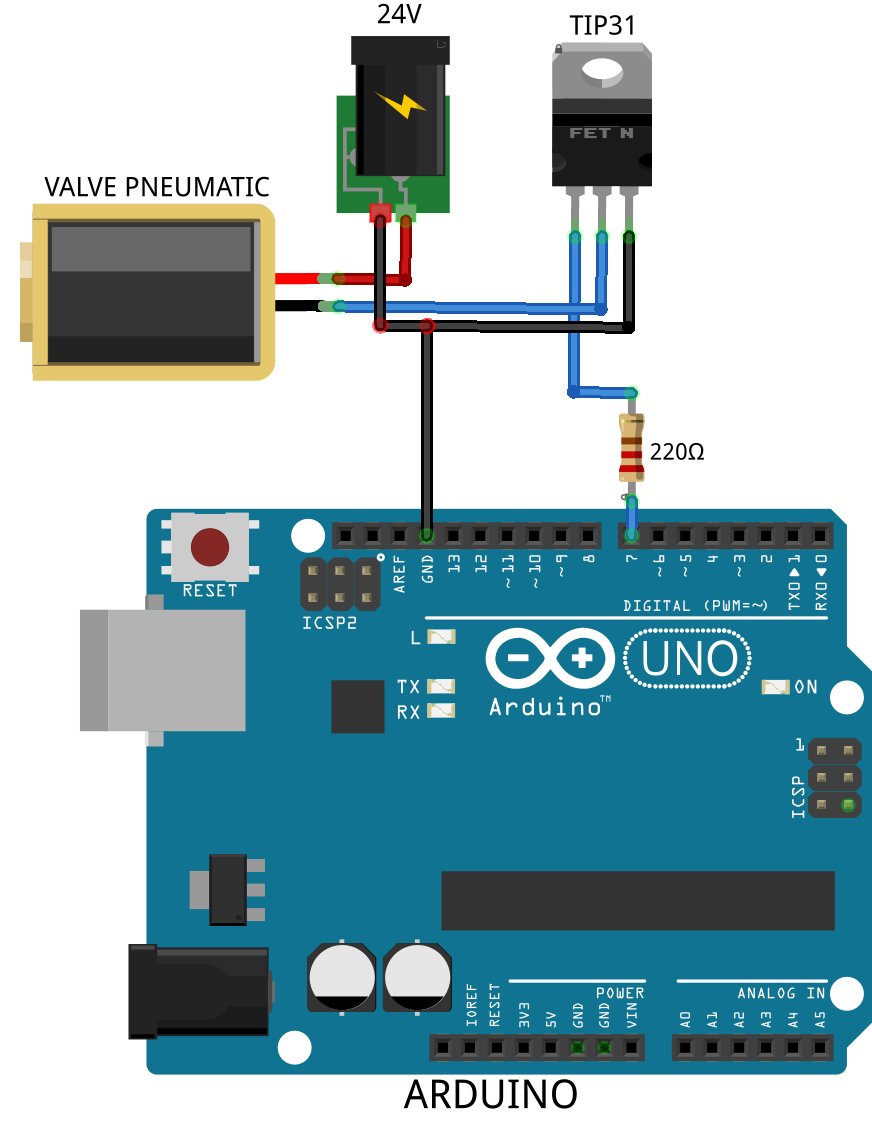
\includegraphics[width=5cm]{gambar/tip31.png}
	\caption{Rangkaian \textit{Valve Pneumatic} dengan Rangkaian TIP31}
	\label{pic.skematikvalve}
\end{figure}
\subsubsection{Rangkaian Minimum Sistem Arduino}
Arduino Mega 2560 digunakan sebagai mikrokontroler utama untuk mengendalikan seluruh sistem pada \textit{arm manipulator robot} SCARA. Arduino  2560 memiliki banyak pin keluaran dan masukan digital dan analog yang dapat digunakan sebagai pengendali fungsi – fungsi dari setiap komponen. Pin pada Arduino  2560 dapat mencukupi kebutuhan masukan dan keluaran untuk sistem kerja robot. Pin analog yang pada Arduino  digunakan untuk menerima \textit{feedback} masukkan dari potensio yang ada pada setiap motor robot. Beberapa pin digital pada Arduino Mega 2560 juga  memiliki fungsi lain yaitu sebagai pin \textit{Pulse With Modulation} (PWM) yang dapat digunakan sebagai keluaran analog sehingga dapat digunakan untuk mengatur nilai tegangan kaluaran dari Arduino  2560. Pin PWM yang cukup digunakan untuk kontrol kecepatan pada \textit{driver} motor. Selain itu pin PWM pada Arduino Mega 2560 digunakan untuk memberikan kontrol direksi pada \textit{driver} motor untuk memberikan masukan arah putar kanan ataupun putar kiri. Gambar \ref{pic.sisminarduino} merupakan rangkaian sistem minimum Arduino Mega 2560 pada robot SCARA ini. Tabel \ref{tbl.pinarduino} merupakan fungsi dari masing-masing pin yang ada pada Arduino Mega 2560.
\begin{figure}[H]
	\centering
	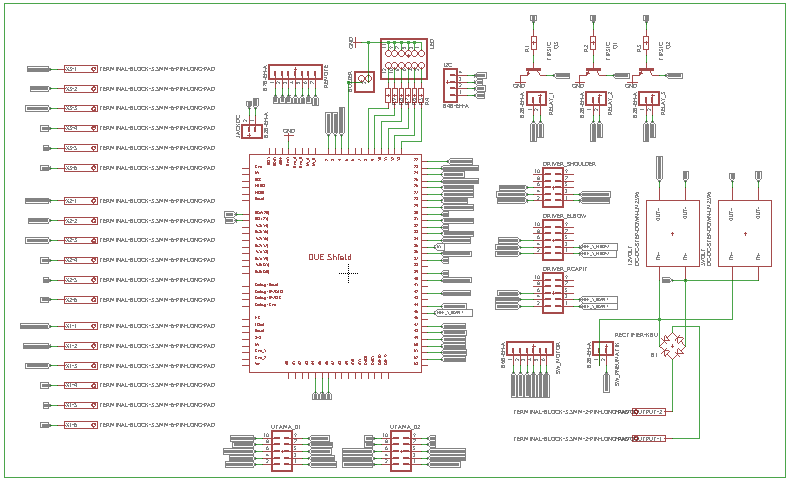
\includegraphics[width=15cm, height=10cm]{gambar/skematik1.png}
	\caption{Rangkaian Minimum Sistem Arduino}
	\label{pic.sisminarduino}
\end{figure}

\begin{table}[H]
		\centering
	\caption{Pin pada Arduino Mega 2560}
	\label{tbl.pinarduino}
	\begin{tabular}{|c|c|l|}
		\hline
		\rowcolor[HTML]{9B9B9B} 
		No & \begin{tabular}[c]{@{}c@{}}Pin Arduino\\   Mega 2560\end{tabular} & \multicolumn{1}{c|}{\cellcolor[HTML]{9B9B9B}Fungsi} \\ \hline
		1  & A1                                                                & Feedback potensiometer shoulder                     \\ \hline
		2  & A2                                                                & Feedback potensiometer elbow                        \\ \hline
		3  & A3                                                                & Feedback potensiometer end-effector                 \\ \hline
		4  & D16, D18                                                          & Kontrol aktif driver motor shoulder                 \\ \hline
		4  & D20, D22                                                          & Kontrol driver motor shoulder                       \\ \hline
		5  & D24, D26                                                          & Kontrol aktif driver motor elbow                    \\ \hline
		6  & D28. D30                                                          & Kontrol driver motor elbow                          \\ \hline
		7  & D32, D34                                                          & Kontrol aktif driver motor end-effector             \\ \hline
		8  & D36, D38                                                          & Kontrol driver motor end-effector                   \\ \hline
		9  & D4                                                                & Kontrol PWM driver motor shoulder                   \\ \hline
		10 & D5                                                                & Kontrol PWM driver motor elbow                      \\ \hline
		11 & D6                                                                & Kontrol PWM driver motor end-effector               \\ \hline
		12 & D7                                                                & Kontrol valve relay naik                            \\ \hline
		13 & D8                                                                & Kontrol valve relay turun                           \\ \hline
		14 & D9                                                                & Kontrol valve relay buka-tutup                      \\ \hline
		15 & D15                                                               & Kontrol LED Shoulder aktif high                     \\ \hline
		16 & D17                                                               & Kontrol LED elbow aktif high                        \\ \hline
		17 & D19                                                               & Kontrol LED end-effector naik aktif high            \\ \hline
		18 & D21                                                               & Kontrol LED end-effector turun aktif high           \\ \hline
		19 & D23                                                               & Kontrol LED end-effector buka-tutup aktif high      \\ \hline
		20 & D25                                                               & Buzzer aktif high                                   \\ \hline
	\end{tabular}
\end{table}

\subsubsection{Rangkaian Catu Daya}
Rangkaian catu daya merupakan hal yang sangat penting dalam sebuah sistem. Pada \textit{arm manipulator robot} SCARA terdapat tiga buah bilai tegangan \textit{supply} yang berbeda. Tegangan yang ditujukkan untuk Arduino Mega 2560 dan beberapa sensor membutuhkan tegangan 5 Volt, motor DC membutuhkan tegangan 12 Volt dan \textit{valve pneumatic} membutuhkan tegangan 24 Volt. Catu daya diawali dengan tegangan AC 220 Volt dari listrik PLN. Tegangan tersebut kemudian diturunkan menggunakan sebuah trafo 3A menjadi 24 Volt AC. Komponen yang digunakan dalam rangakaian merupakan komponen yang membutuhkan tegangan DC, maka tegangan 24 Volt AC diubah menjadi 24 DC menggunakan rangkaian dioda \textit{bridge}. Tegangan 24 Volt DC diarahkan menuju dua buah regulator \textit{Buck} LM2596 yang masing-masing menghasilkan tegangan 12 Volt dan 5 Volt. Gambar \ref{pic.skematikcatu} merupakan rangkaian catu daya secara keseluruhan.
\begin{figure}[H]
	\centering
	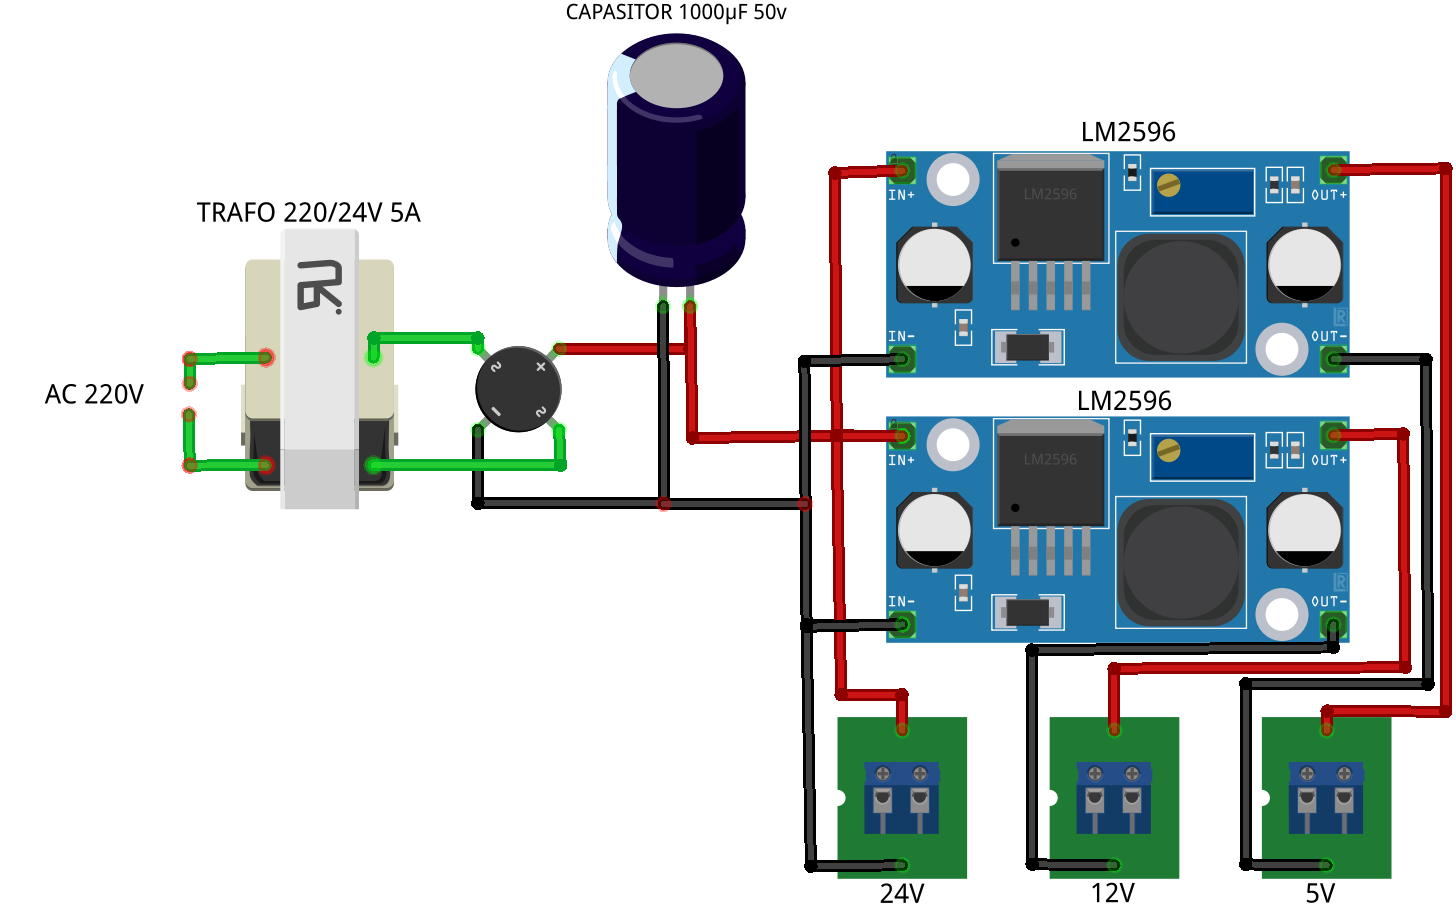
\includegraphics[width=8cm]{gambar/catudaya_bb.png}
	\caption{Rangkaian Catu Daya}
	\label{pic.skematikcatu}
\end{figure}
\section{Perancangan Perangkat Lunak}
Perangkat lunak yang digunakan merupakan \textit{software} Processing IDE. Processing IDE diprogram agar mendapatkan sebuah GUI yang cocok sesuai dengan fungsi robot SCARA. Di dalam GUI terdapat dua bagian yang diantaranaya merupakan bagian kontrol, dan bagian \textit{display}. Pada bagian kontrol nantinya dalam GUI akan mengkontrol mulai dari pergerakan dan posisi dari robot SCARA. Sedangkan pada bagian penampil, GUI menampilkan nilai dari sudut, posisi, serta animasi terkait robot SCARA. Gambar 3.21 merupakan tampilan dari GUI secara keseluruhan. Tabel 3.21 menyajikan setiap komponen yang ditampilan di dalam GUI processing IDE.
\begin{figure}[H]
	\centering
	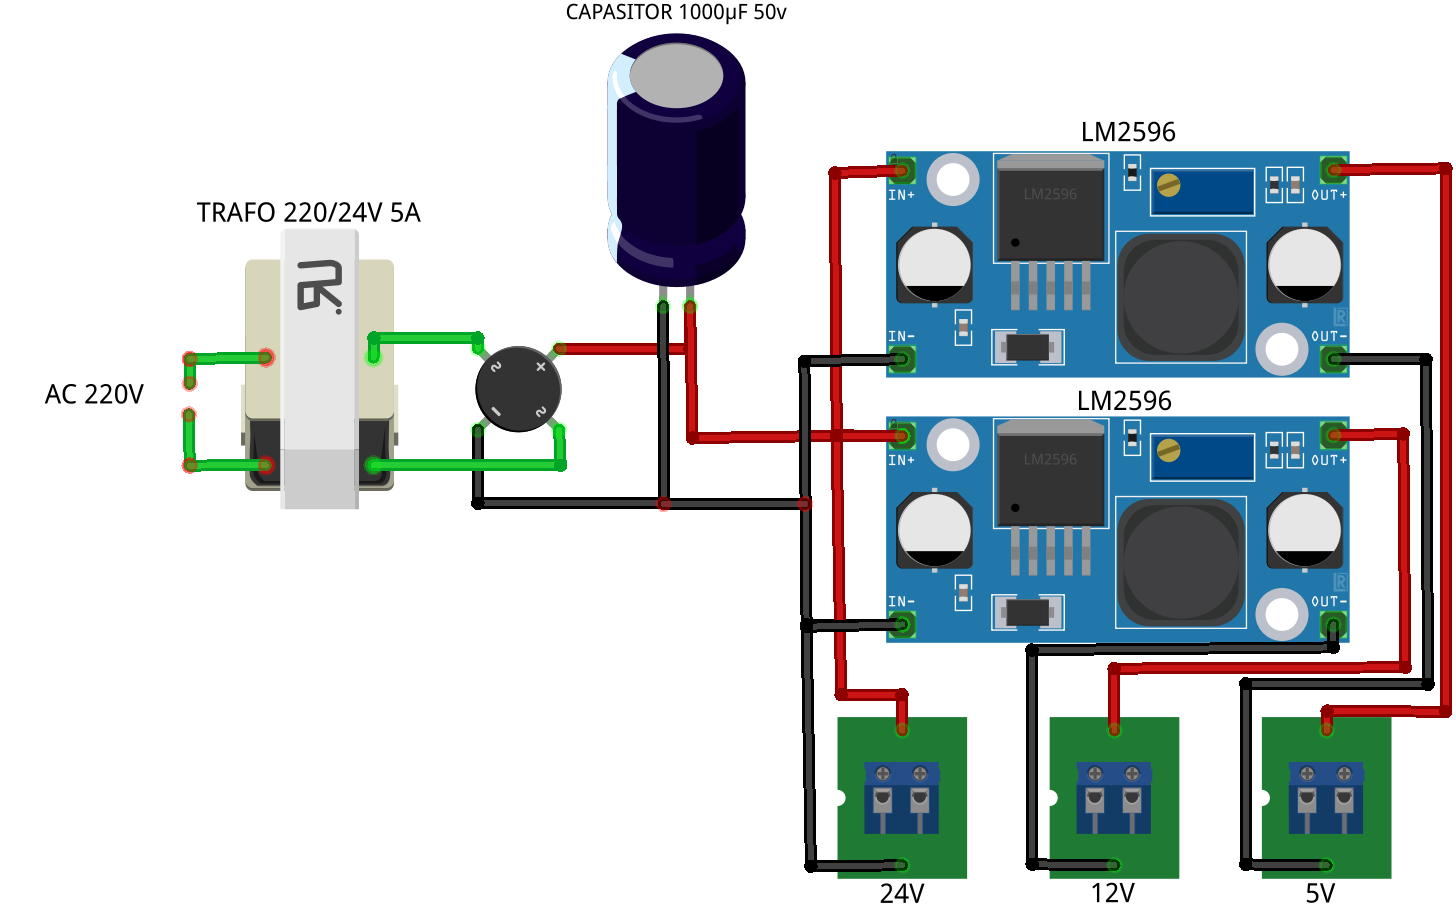
\includegraphics[width=10cm ]{gambar/catudaya_bb.png}
	\caption{Tampilan GUI Sistem Kinematika Robot SCARA}
\end{figure}

\begin{table}[H]
	\centering
	\caption{Keterangan Tampilan pada GUI Robot SCARA}
	\begin{tabular}{|c|c|l|}
		\hline
		\rowcolor[HTML]{9B9B9B} 
		No & \begin{tabular}[c]{@{}c@{}}Pin Arduino\\   Mega 2560\end{tabular} & \multicolumn{1}{c|}{\cellcolor[HTML]{9B9B9B}Fungsi} \\ \hline
		1  & A1                                                                & Feedback potensiometer shoulder                     \\ \hline
		2  & A2                                                                & Feedback potensiometer elbow                        \\ \hline
		3  & A3                                                                & Feedback potensiometer end-effector                 \\ \hline
		4  & D16, D18                                                          & Kontrol aktif driver motor shoulder                 \\ \hline
		4  & D20, D22                                                          & Kontrol driver motor shoulder                       \\ \hline
	
	\end{tabular}
\end{table}


\subsection{ControlP5}
ControlP5 merupakan salah satu library yang berguna dalam membuat sebuah GUI. Dalam library yang disediakan terdapat banyak pilihan terkait kontrol sistem dengan berbagai jenis pilihan. Kontrol sistem yang disediakan tersedia dua pilihan yaitu untuk menkontrol dan untuk menampilkan sebuah data. Masing-masing kontrol sistem ini dapat digunakan dengan cara memanggilnya pada program yang ditulis.

Pada perancangan kineatika roboto scara ini, menggunakan empat buah kontrol sistem. Empat kontrol sistem yang digunakan merupakan jenis kontrol sistem yang berguna untuk memberikan sebuah data yang dikirimkan pada Arduino Mega 2560. Kontrol sistem tersebut diantaranya:
\begin{enumerate}
	\item \textit{Slider Control} \\
	\textit{Slider Control} berupa tampilan kontrol GUI yang menggunakan sistem geser dalam memberikan data. Data memiliki batasan atas dan batas bawah yang dimasukkan dalam program. Keuntungan menggunakan kontrol sistem jenis ini karena saat ingin untuk mengubah data yang diberikan menjadi lebih mudah.


	\item \textit{Textfield Control} \\
\textit{Textfield control} berupa tampila kontrol GUI yang menggunakan masukan nilai data sesuai apa yang dituliskan atau diketikkan secara langsung. Kelebihan menggunakan kontrol sistem jenis ini karena dapat memasukkan nilai data lebih spesifik secara langsung sesuai keiinginan.
	
	\item \textit{Textfield Control} \\
\textit{Bang control}
Berbeda dengan kontrol sistem sebelumnya,\textit{ bang control }berupa kotak yang bekerja pada saat mulai ditekan. Saat bang mulai ditekan data akan dikirimkan sesuai dengan nilai yang sudah dimasukan kedalam program. 
	

	\item \textit{Textfield Control} \\
\textit{Toggle control}
Toggle control memiliki sistem kontrol seperti saklar on-off. Pada saat ditekan maka toggle control menyimpan data berupa kondisi pertama dan berubah saat ditekan kembali. 

\end{enumerate}
\subsection{Shape}
Shape pada GUI berfungsi sebagai penampil secara tiga dimensi dari robot SCARA. Robot SCARA dapat ditampilkan dalam berbagai ukuran, letak dan juga dapat bergerak sesuai dengan data yang diberikan. Pergerakan dari robor SCARA merupakan implementasi dari wujud aslinya yang pergerakannya sama.

Dalam pengoperasianya, desain dari robot SCARA yang ditampilkan harus dimasukkan ke dalam folder yang sama dengan program processing IDE. File yang dapat ditampilkan merupakan file dengan jenis obj. yang berarti file objek. Pada program robot SCARa file dari dimensi tiga dari robot SCARA memiliki tiga buah file dimana ketiganya adalah \textit{base, shoulder}, dan \textit{elbow}. 

\section{Sistem Kinematika}
Persamaan kinematika terbagi dua, yaitu kinematika maju dan kinematika balik. Kinematika maju digunakan untuk menentukan posisi dan orientasi \textit{end-effector} apabila variabel sudut \textit{joint}-nya telah diketahui. Kinematika balik digunakan untuk mencari \textit{joint} robot daam menentukan posisi dan orientasi dari \textit{end-effector.}
\subsection{Prinsip Kerja Kinematika Maju}
Metode Denavit-Hartenberg merupakan metode yang menggabungkan proses perhitungan rotasi dan translasi menjadi sebuah matriks yang menyertakan nilai-nilai sudut putar dan jarak sendi dari sebuah lengan robot. Dalam beberapa aplikasi, metode Denavit-Hartenberg umumnya digunakan dalam perhitungan \textit{Forward Kinematics}. Dalam penelitian ini dirancang aplikasi yang menggunakan metode Denavit-Hartenberg untuk menghitung sudut-sudut tiap sendi pada \textit{Invers Kinematics} untuk menggerakan sebuah lengan robot. Matrik Denavit-Hartenberg yang berisi perhitungan rotasi dan translasi digunakan untuk mendapatkan nilai nilai sudut untuk menggerakkan tiap motor sendi. Empat Aturan Frame Denavit-Hartenberg yaitu Sumbu Z harus menjadi sumbu rotasi atau translasi dari sebuah joint. Sumbu X harus tegak lurus dari sumbu Z frame sebelumnya. Sumbu X harus memotong atau menyilang dari sumbu Z frame sebelumnya. Sumbu Y harus digambarkan sesuai dengan aturan tangan kanan setelah sumbu X   dan sumbu Z setiap frame digambarkan.
\subsection{Prinsip Kerja Kinematika Balik}
Dalam menentukan koordinat \textit{end-effector}, kinematika balik harus disesuaikan dengan batas area kerja \textit{(workspace)} dari jangkauan robot. Kinematika balik adalah perhitungan untuk mencari variabel sudut (\textit{joint}) robot dalam menentukan posisi dan orientasi dari \textit{end-effector}. Penyelesaian kinematika balik ini dapat diselesaikan dengan menggunakan kinematika balik, yang di dalamnya menggunakan hukum \textit{phytagoras} dan aturan \textit{cosinus}. 
Secara garis besar metode \textit{inverse kinematic} akan mencari nilai-nilai parameter yang harus diberikan kepada setiap aktuator untuk mencapai tujuan akhir. Untuk mendapatkan nilai-nilai parameter tersebut, robot harus mengetahui terlebih dahulu manipulator yang dimilikinya, baik ukuran maupun jumlah aktuator serta derajat kebebasan yang ada. Kemudian, robot harus ditanamkan rumus-rumus yang didapat dari berbagai model perhitungan, baik dari segi analisa grafik langsung maupun menggunakan metode-metode dari berbagai penelitian. 

Analisis persamaan kinematik dapat diselesaikan dengan cara yang paling dasar yaitu menggunakan trigonometri dengan bantuan grafik. Pada penelitian ini karena menggunakan sebuah GUI yang didalamnya terdapat animasi dari bentuk fisik robot SCARA maka koordinat didapat dari processing IDE. Robot SCARA yang terdapat di dalam processing IDE menggunakan skala tertentu agar menarik dalam tampilan dan tetap sesuai dari dimensi aslinya. Penyelesaian kinematika dalam robot SCARA cukup diselesaiakan menggunakan satu sisi, yaitu sisi atas (\textit{top view}) dari struktur robot lengan. Pada sisi atas derajat sudut \textit{joint} \textit{shoulder}, dan sudut \textit{joint elbow} dapat ditemukan. Persamaan kinematika balik untuk sisi atas dapat dilihat pada Gambar 3.17.
\begin{figure}[H]
	\centering
	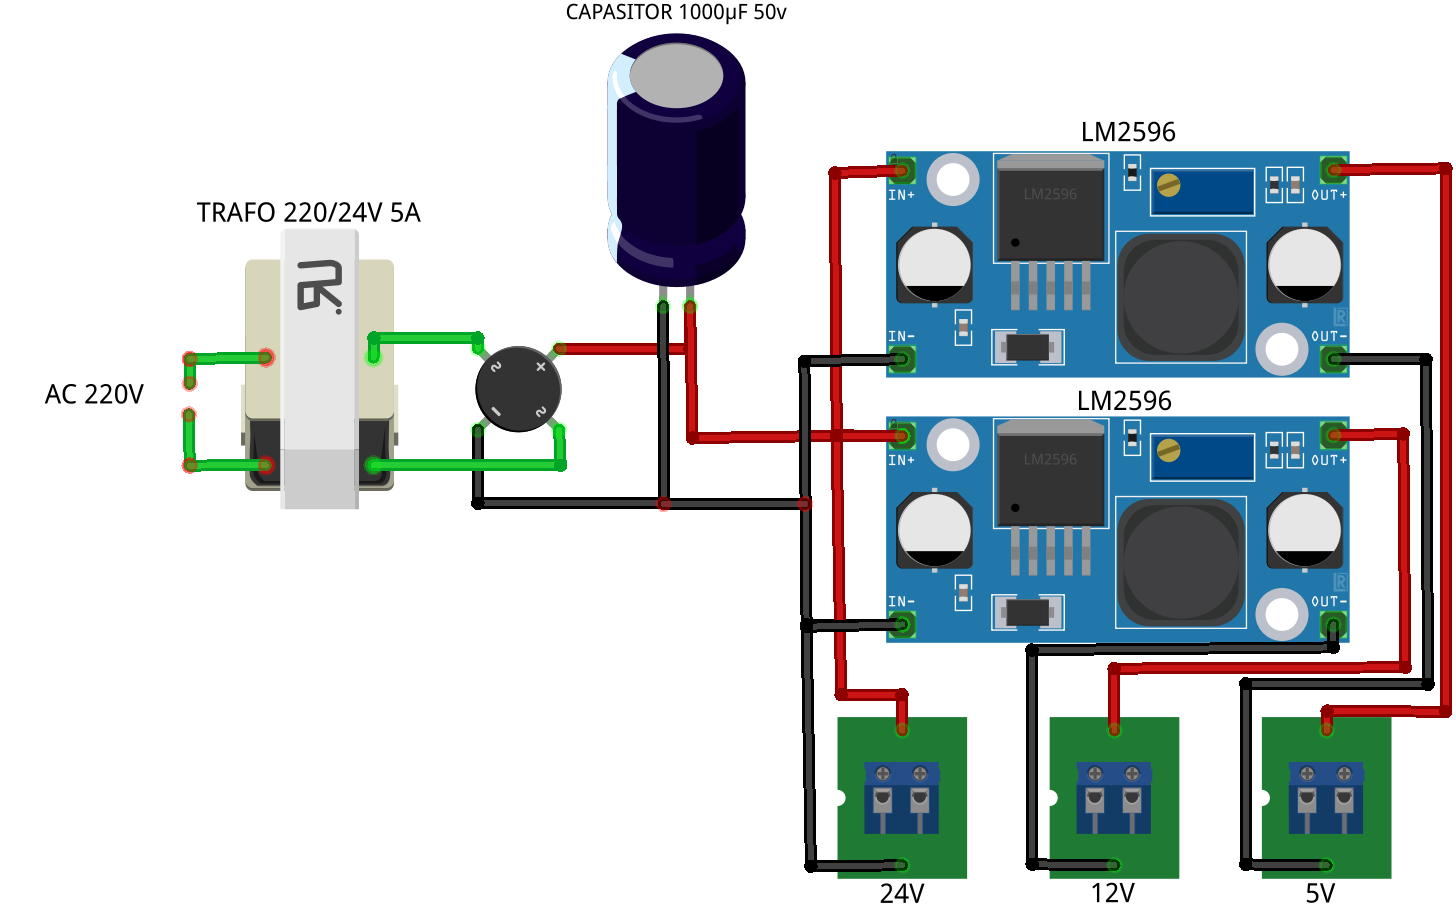
\includegraphics[width=8cm]{gambar/catudaya_bb.png}
	\caption{Trigonometeri Sisi Atas}
	\label{g_ik}
\end{figure}
 
 
Pada robot SCARA, sudut dari \textit{joint} yang dicari merupakan \textit{joint} dari \textit{shoulder} dan juga \textit{elbow.} Kedua \textit{joint} tersebut dapat ditemukan dengan melalui persamaan \textit{pythagoras} dan juga hukum \textit{cosinus}. Pada Gambar 3.17 terlihat bahwa sudut \textit{shoulder} merupakan besar sudut diantara lengan \textit{shoulder} dan juga sumbu x dan sudut elbow merupakan besar sudut antara lengan \textit{elbow} dengan garis bantu dari lengan \textit{shoulder}. Keduanya dapat ditentukan besar nilainya melalui beberapa pesamaan dari \textit{cosinus} dan juga hukum \textit{pyhtagoras}. $l_{1}$ merupakan panjang lengan \textit{shoulder} dan $l_{2}$ merupakan panjang lengan dari \textit{elbow}. Serta $\theta_{1}$ merupakan sudut dari shoulder dan $\theta_{2}$ merupakan sudut dari \textit{elbow}.  

\begin{enumerate}
	\item Dengan menggunakan hukum \textit{cosinus}, didapatkan sebuah persamaan \ref{cosinus1}
	\begin{equation}
	(x^2+y^2)=l_{1}^2+l_{1}^2-2l_{2}l_{2}cos(180-\theta_{2})
	\label{cosinus1}
	\end{equation}
	\item Pada persamaan \ref{cosinus2} terdapat $\cos$ yang dapat diubah sesuai dengan prinsip dari hukum \textit{cosinus} menjadi seperti pada persamaan \ref{cosinus2}
	\begin{equation}
	(x^2+y^2)=l_{1}^2l_{2}^2+2l_{2}l_{2}cos(\theta_{2})
	\label{cosinus2}
	\end{equation}
	\item Pada persamaan \ref{cosinus2} mencari sebuah nilai dari $\theta_{2}$ untuk memmudahkannya maka persamaan menjadi seperti pada persamaan \ref{cosinus3}
	\begin{equation}
	cos(\theta_{2})=\frac{x^2+y^2-l_{1}^2-l_{2}^2}{2_{1}l_{2}}
	\label{cosinus3}
	\end{equation}
	\item Nilai dari $\theta_{2}$ dapat dengan mudah diketahui dengan melanjutkan seperti pada persamaan \ref{cosinus4}
	\begin{equation}
	\theta_{2}=arccos(\frac{x^2+y^2-l_{1}^2-l_{2}^2}{2_{1}l_{2}})
		\label{cosinus4}
	\end{equation}
	Dengan persamaan \ref*{cosinus4} maka nilai dari $\theta_{2}$ atau sudut dari \textit{elbow} dapat diketahui dengan cara memasukkan nilai posisi x, posisi y, serta panjang dari \textit{shoulder} dan \textit{elbow} ke dalam persamaan. Nilai posisi x dan posisi y merupakan posisi akhir dari \textit{end-effector}. 
	\item Dalam menentukan sudut lainnya yaitu sudut \textit{shoulder} yang ditandai dengan simbol $\theta_{1}$ menggunakan persamaan \textit{cosinus} yang dituliskan pada persamaan \ref{cosinus5}
	\begin{equation}
	\frac{sin(\beta)}{l_{2}} = \frac{sin(\gamma)}{\sqrt{x^2+y^2}} ; \alpha=\arctan(\frac{y}{x})
	\label{cosinus5}
	\end{equation}
	\item Pada persamaan \ref{cosinus5} $\sin(\gamma)=\sin(180-\theta_{2})=\sin(\theta_{2})$ dengan mengubah $\sin(\gamma)$ menjadi $\sin(\theta_{2})$ maka akan persamaan menjadi seperi yang ditunjukkan pada persamaan \ref{cosinus6}
	\begin{equation}
	\beta=\arcsin(\frac{l_{2}\sin(\theta_{2})}{\sqrt{x^2+y^2}})
	\label{cosinus6}
	\end{equation}
	\item Jika dilihat pada persamaan \ref{g_ik} makan besar dari sudut \textit{shoulder} yang ditandakan dengan $\theta_{1}$ yang berarti $\theta_{1}=\beta+\alpha$ maka dapat diselesaikan dengan persamaan \ref{cosinus7}
	\begin{equation}
	\theta_{1}=\arcsin(\frac{l_{2}\sin(\theta_{2})}{\sqrt{x^2+y^2}}+\arctan(\frac{y}{x})
	\label{cosinus7}
	\end{equation}
	\item  Dengan penyelesaian seperti pada persamaan \ref{cosinus7} besar sudut dari \textit{shoulder} dapat diketahui dengan memasukkan nilai panjang \textit{elbow}, sudut \textit{elbow} dan juga posisi dari \textit{end-effector}.
\end{enumerate}

Pada dalam penelitian kinematika robot SCARA ini, segala perhitungan kinematika dilakukan di dalam program processing IDE. Di dalam processing IDE terdapat animasi dari bentuk asli robot SCARA dengan dimensi yang sama hanya saja ditampilkan dalam bentuk berskala. Pada posisi \textit{end-effector} didapat posisi x dan y yang diprogram pada dalam processing IDE. Dua buah data sudut yang didapat pada perhitungan sudut \textit{shoulder} dan \textit{elbow} kemudian dikirimkan kepada Arduino Mega 2560 untuk diprores dan diimplemintasikan secara langsung pada robot yang asli.

\section{Perancangan Sistem Keseluruhan}
Rancangan sistem keseluruhan merupakan gabungan dari perancangan perangkat keras dan perangkat lunak yang diintegrsikan sesuai dengan diagram blok sistem. Gambar 3.20 adalah gambaran tentang perancangan sistem secara keseluruhan. Tabel 3.3  menunjukkan keterangan setiap komponen yang ada di dalam sistem keseluruhan \textit{arm manipulator} robot SCARA. 
\begin{figure}[H]
	\centering
	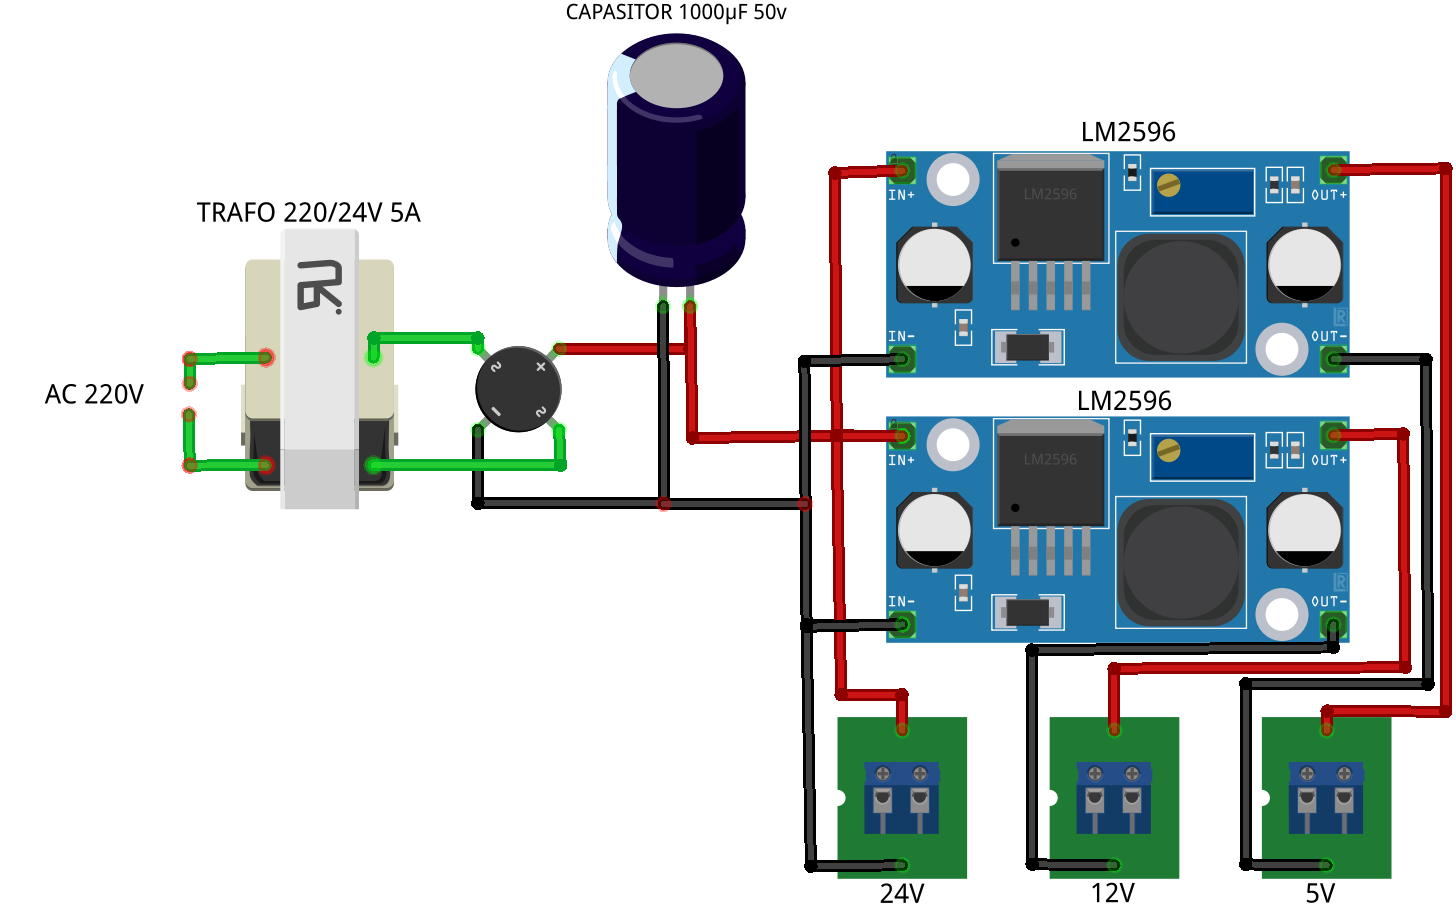
\includegraphics[width=8cm]{gambar/catudaya_bb.png}
	\caption{Sistem Secara Keseluruhan}
	\label{g_ik}
\end{figure}

\begin{table}[H]
	\centering
	\caption{Keterangan Sistem Keseluruhan}

		\begin{tabular}{|c|l|}
			\hline
			\rowcolor[HTML]{9B9B9B} 
			No & \multicolumn{1}{c|}{\cellcolor[HTML]{9B9B9B}Keterangan} \\ \hline
			1  & Robot Lengan SCARA                                      \\ \hline
			2  & Box Panel                                               \\ \hline
			3  & Arduino Mega 2560                                       \\ \hline
			4  & Personal Computer                                       \\ \hline
			5  & GUI Processing IDE                                      \\ \hline
			6  & Workspace Robot SCARA                                   \\ \hline
			7  & Kompresor                                               \\ \hline
			8  & Objek                                                   \\ \hline
		\end{tabular}

\end{table}
Processing IDE merupakan piranti yang digunakan sebagai masukan. Masukan dari Processing IDE adalah hasil dari perhitungan kinematika maju dan atau kinematika balik yang dimasukkan melalui GUI. Objek berada dalam cakupan \textit{workspace} yang telah ditentukan luasnya yang ditinjau dari cangkupan dari \textit{end-effector}. GUI dari processing IDE ini diproses menggunakan komputer personal.  

Processing IDE juga menampilan nilai derajat setiap \textit{joint}, koordinat x dan y dari \textit{end-effector}. Koordinat x dan y yang telah didapatkan dari processing IDE diolah dalam perhitungan kinematika balik sehingga dapat ditemukan nilai besar derajat sudut setiap joint. Setelah nilai besar derajat sudut setiap \textit{joint} didapatkan, Processing IDE akan mengirimkan nilai-nilai tersebut ke Arduino IDE melewati komunikasi Serial. Arduino IDE akan mengirimkan nilai-nilai tersebut sesuai dengan pin motor DC yang tersambung dengan Arduino Mega 2560, lalu nilai-nilai \textit{joint}  tersebut dikirimkan Arduino Mega 2560 kembali ke processing IDE melaluo koneksi langsung menggunakan kabel USB.  

Arduino Mega 2560 merupakan mikrokotroler yang menggerakkan setiap motor DC sesuai dengan besaran nilai yang telah didapatkan. Setelah itu, robot lengan SCARA akan mencapai koordinat x dan y dari objek, lalu mencengkram objek tersebut dengan \textit{Gripper}.


\chapter{PENGUJIAN DAN PEMBAHASAN}
Pada bab pengujian dan pembahasan ini, penulis akan melakukan pengujian sistem kendali\textit{ arm manipulator} robot SCARA berdasarkan spesifikasi sistem yang telah dijelaskan pada bab sebelumnya. Tujuan pengujian ini adalah untuk membuktikan apakah sistem yang diimplementasikan telah memenuhi spesifikasi dan rancangan yang sudah direncanakan sebelumnya. Hasil dari pengujian akan dimanfaatkan untuk menyempurnakan kinerja dari sistem dan sekaligus digunakan dalam pengembangan sistem lebih lanjut. Metode pengujian dipilih berdasarkan fungsionalitas dan beberapa parameter yang ingin diketahui dari sistem tersebut. Data yang diperoleh dari metode pengujian yang dipilih tersebut dapat memberikan informasi yang cukup dan dapat digunakan untuk penyempurnaan dan pengembangan sistem.

Metode pengujian menggunakan dua macam metode, yaitu pengujian fungsionalitas dari setiap komponen dan pengujian sistem secara keseluruhan. Pengujian fungsionalitas digunakan untuk membuktikan apakah sistem yang diimplementasikan dapat memenuhi persyaratan dari fungsi operasional yang telah dirancang dan direncanakan sebelumnya. Sedangkan pengujian sistem secara keseluruhan bertujuan untuk memperoleh beberapa parameter yang dapat menunjukkan kemampuan dan keandalan dari sistem secara keseluruhan dalam menjalankan fungsi operasionalnya. Pada \textit{sistem arm manipulator} robot SCARA dilakukan terlebih dahulu pengujian terhadap fungsional dari beberapa komponen seperti bagian \textit{DC to DC converter}, arah gerakan motor DC, \textit{feedback} potensiometer, fungsi rangkaian \textit{switching} pada \textit{valve pneumatic} dan keakuratan setiap \textit{joint} untuk bergerak sesuai sudut yang diinginkan berdasarkan kinematika balik maupun kinematika maju dengan menggunakan kontrol dari GUI.  Kemudian setelah pengujian fungsional terpenuhi maka dilakukan pengujian sistem secara keseluruhan untuk mengetahui keakuratan dan keandalan dari sistem \textit{arm manipulator} robot SCARA.

\section{Pengujian Fungsional}
Pengujian fungsional digunakan untuk menguji bagian – bagian dari sistem yang terdiri dari\textit{DC to DC converter}, arah gerakan motor DC, \textit{feedback} potensiometer, fungsi rangkaian \textit{switching} pada \textit{valve pneumatic} dan keakuratan setiap \textit{joint}, pengujian GUI Processing dan pengujian program. 

\subsection{Pengujian DC - to - DC Converter}
Pengujian DC – to – DC \textit{converter} dilakukan untuk mengetahui tegangan masukan pada Arduino Mega 2560, sensor \textit{potensiometer}, motor DC dan juga sumber tegangan untuk\textit{ valve pneumatic}. Tegangan masukan dari catu daya utama sebesar 24 Volt DC yang nantinya dibagi ke tiga buah nilai tegangan. Tabel 4.1 merupakan tegangan keluaran DC – to - DC.

\begin{table}[H]
	\centering
	\caption{Hasil Tegangan Keluaran Dari Tegangan DC-DC Converter}
	
	\begin{tabular}{|c|l|}
		\hline
		\rowcolor[HTML]{9B9B9B} 
		No & \multicolumn{1}{c|}{\cellcolor[HTML]{9B9B9B}Keterangan} \\ \hline
		1  & Robot Lengan SCARA                                      \\ \hline
		2  & Box Panel                                               \\ \hline
		3  & Arduino Mega 2560                                       \\ \hline
		4  & Personal Computer                                       \\ \hline
		5  & GUI Processing IDE                                      \\ \hline
		6  & Workspace Robot SCARA                                   \\ \hline
		7  & Kompresor                                               \\ \hline
		8  & Objek                                                   \\ \hline
	\end{tabular}
	
\end{table} 

Pada saat mengubbah besar tegangan keluaran yang dilakukan oleh Regulator \textit{Buck} LM2596 dilakukan dengan cara memutar \textit{potensiometer} yang terdapat pada Regulator \textit{Buck}. Diputar searah dengan jarum jam sesuai hingga pada teganangan yang diinginkan.
\subsection{Pengujian Motor DC}
Pengujian motor DC dilakukan untuk mengetahui apakah motor DC dalam keaadaan baik atau tidak. Pengujian dilakukan dengan memberikan tegangan kerja pada motor DC yang ada pada \textit{shoulder}, \textit{elbow}, dan juga \textit{end-effector} yang nantinya diukur arus yang dihasilkan pada masing-masing motor DC. Tabel \ref{tbl.motordc} merupakan hasil dari pengujian pada masin-masing motor DC.

\begin{table}[H]
	\centering
	\caption{Hasil Tegangan Keluaran Dari Tegangan DC-DC \textit{Converter}}
	
	\begin{tabular}{|c|l|}
		\hline
		\rowcolor[HTML]{9B9B9B} 
		\label{tbl.motordc}
		No & \multicolumn{1}{c|}{\cellcolor[HTML]{9B9B9B}Keterangan} \\ \hline
		1  & Robot Lengan SCARA                                      \\ \hline
		2  & Box Panel                                               \\ \hline
		3  & Arduino Mega 2560                                       \\ \hline
		4  & Personal Computer                                       \\ \hline
		5  & GUI Processing IDE                                      \\ \hline
		6  & Workspace Robot SCARA                                   \\ \hline
		7  & Kompresor                                               \\ \hline
		8  & Objek                                                   \\ \hline
	\end{tabular}
	
\end{table} 

Pada hasil yang ditunjukkan oleh tabel \ref{tbl.motordc} menujukkan bahwa setiap motor DC mempunyai nilai arus yang berbeda-beda. Motor DC yang terletak pada \textit{end-effcetor} merupakan motor DC yang menghasilkan arus paling besar. Hal ini disebabkan karena motor DC yang terpasang pada \textit{end-effector} dibantu dengan bantuan \textit{belt} untuk menyalurkan putaran pada\textit{ end-effector}. Dengan begitu penggunaan \textit{belt} pada motor DC ini menyebabkan beban yang dikerjakan oleh motor DC pada \textit{end-effector} menjadi lebih besar dari pada motor DC yang lain yang langsung menggerakkan pada masing-masing \textit{joint}.

\subsection{Pengujian \textit{Driver} Motor H – \textit{Bridge}}
Pengujian \textit{driver} motor H – \textit{bridge} dilakukan untuk mengetahui keberfungsian dari \textit{driver} motor apakah sesuai dengan perancangan atau tidak. Pada \textit{driver} motor juga dilakukan pengujian untuk melihat direksi dari arah pergerakan motor DC dari \textit{output} \textit{driver} ketika diberikan masukan berupa sinyal \textit{high} dan \textit{low} pada arduino. Tabel \ref{tbl.drivermotor} menunjukkan hasil dari pengujian \textit{driver} motor H-\textit{Bridge}. 
\begin{table}[H]
	\centering
	\caption{Hasil Pengujian \textit{Driver} Motor H-\textit{Bridge}}
		\label{tbl.drivermotor}
	\begin{tabular}{|c|l|}
		\hline
		\rowcolor[HTML]{9B9B9B} 
	
		No & \multicolumn{1}{c|}{\cellcolor[HTML]{9B9B9B}Keterangan} \\ \hline
		1  & Robot Lengan SCARA                                      \\ \hline
		2  & Box Panel                                               \\ \hline
		3  & Arduino Mega 2560                                       \\ \hline
		4  & Personal Computer                                       \\ \hline
		5  & GUI Processing IDE                                      \\ \hline
		6  & Workspace Robot SCARA                                   \\ \hline
		7  & Kompresor                                               \\ \hline
		8  & Objek                                                   \\ \hline
	\end{tabular}
	
\end{table} 

 Pada \textit{driver} motor H-\textit{Bridge} EMS 30A sinyal digital \textit{high} dan \textit{low} dihubungkan pada pin MEN1 dan MEN2. Dari hasil pengujian \textit{driver} motor H-\textit{Bridge} seperti yang ditunjukkan pada tabel \ref{tbl.drivermotor} terlihat bahwa ketika sinyal \textit{high} diberikan pada MEN1 dan \textit{low} diberikan MEN2 maka pergerakan motor akan berputar searah dengan arah jarum jam dan sebaliknya jika diberikan \textit{low} pada MEN1 dan \textit{high} pada MEN2 maka arah pergerakan motor akan berlawanan arah. Pada tabel \ref{tbl.drivermotor}juga terlihat bahwa nilai arus dapat dialirkan pada driver motor beragam dari 1 Ampere hingga 1.5 Ampere. Terbukti bahwa \textit{driver} motor dapat mengoperasikan driver motor dengan baik.

\subsection{Pengujian Nilai\textit{ Analog Potensiometer}}
Pengujian nilai \textit{analog potensiometer} berfungsi untuk mengetahui apakah \textit{potensiometer} bekerja dengan baik dan nilai yang diberikan dalam keadaan yang normal. Pada \textit{potensiometer} nilai data yang dikirimkan berupa data analog yang dihasilkan oleh pembagian tegangan yang diatur pada setiap putaran resistornya. Tegangan yang diberikan awal yaitu 5 Volt kemudian akan dikirimkan kurang dari 5 Volt sesuai dengan posisi pada \textit{potensiometer}. Dengan begitu, posisi ini dapat diimplemantasikan kepada \textit{joint} pada robot SCARA dengan cara mengatur batasan minimal dan maksimal melalui program arduino. Pada hasil akhirnya nilai data yang dikirimkan oleh \textit{potensiometer} kemudian dilakukan \textit{mapping} data sesuai besaran sudut yang dapat dilakukan oleh \textit{joint} yaitu dari 0-360 derajat. Pada tabel \ref{tbl.potensio}  merupakan hasil pengujian dari \textit{potensiometer}.

\begin{table}[H]
	\centering
	\caption{Hasil Pengujian \textit{Potensiometer}}
	\label{tbl.potensiometer}
	\begin{tabular}{|c|l|}
		\hline
		\rowcolor[HTML]{9B9B9B} 
		
		No & \multicolumn{1}{c|}{\cellcolor[HTML]{9B9B9B}Keterangan} \\ \hline
		1  & Robot Lengan SCARA                                      \\ \hline
		2  & Box Panel                                               \\ \hline
		3  & Arduino Mega 2560                                       \\ \hline
		4  & Personal Computer                                       \\ \hline
		5  & GUI Processing IDE                                      \\ \hline
		6  & Workspace Robot SCARA                                   \\ \hline
		7  & Kompresor                                               \\ \hline
		8  & Objek                                                   \\ \hline
	\end{tabular}
	
\end{table} 

Pada hasil pengujian yang ditunjukkan oleh Tabel \ref{tbl.potensiometer} terlihat bahwa pada saat nilai-niali tertentu, \textit{potensiometer} belum dapat mengirimkan nilai data analog yang berubah-ubah. Hal tersebut dipengaruhi oleh pembacaan \textit{potensiometer} yang belum stabil. Untuk membuat data analog yang dikirimkan oleh \textit{potensiometer} menjadi lebih stabil maka pada program arduino ditambahkan program \textit{moving avarage}. \textit{Moving avarage} berfungi untuk membuat rata-rata nilai dari hasil data pembacaan nilai data pada \textit{potensiometer} yang menyebabkan nilai menjadi lebih stabil. Tabel \ref{tbl.potensiometer2} merupakan hasil pengujian nilai data analog \textit{potensiometer} setelah dilakukan \textit{moving avarage.}

\begin{table}[H]
	\centering
	\caption{Hasil Pengujian \textit{Potensiometer} Menggunakan Program \textit{Moving Avarage}}
	\label{tbl.potensiometer2}
	\begin{tabular}{|c|l|}
		\hline
		\rowcolor[HTML]{9B9B9B} 
		
		No & \multicolumn{1}{c|}{\cellcolor[HTML]{9B9B9B}Keterangan} \\ \hline
		1  & Robot Lengan SCARA                                      \\ \hline
		2  & Box Panel                                               \\ \hline
		3  & Arduino Mega 2560                                       \\ \hline
		4  & Personal Computer                                       \\ \hline
		5  & GUI Processing IDE                                      \\ \hline
		6  & Workspace Robot SCARA                                   \\ \hline
		7  & Kompresor                                               \\ \hline
		8  & Objek                                                   \\ \hline
	\end{tabular}
	
\end{table} 

\subsection{Pengujian Rangkaian Switching Valve Pneumatic}
Pengujian rangkaian \textit{switching} berfungsi untuk mengetahui apakah rangkaian dapat bekerja dengan baik. Fungsi utama dari rangkaian \textit{switching} yang diperuntukkan untuk \textit{valve pneumatic} yaitu sebagai saklar penghubung dan pemutus daya yang masuk untuk \textit{valve pneumatic}. Rangkaian dapat memutus dan menghubungkan daya dengan \textit{trigger} dari sinyal data yang diberikan kepada \textit{Gate} yang berupa sinyal digital \textit{High} dan \textit{Low} dari Arduino Mega 2560. Pengujian dilakukan dengan mengukur keberhasilan rangkaian sebagai rangkaian \textit{switching} dengan variasi tegangan yang dilewatkan. Tabel \ref{tbl.rangkaiantip} merupakan hasil pengujian dari rangkaian \textit{switching} yang diotaki oleh TIP31.
\begin{table}[H]
	\centering
	\caption{Hasil Pengujian Rangkaian \textit{Switching Vavle Pnemuatic}}
	\label{tbl.rangkaiantip}
	\begin{tabular}{|c|l|}
		\hline
		\rowcolor[HTML]{9B9B9B} 
		
		No & \multicolumn{1}{c|}{\cellcolor[HTML]{9B9B9B}Keterangan} \\ \hline
		1  & Robot Lengan SCARA                                      \\ \hline
		2  & Box Panel                                               \\ \hline
		3  & Arduino Mega 2560                                       \\ \hline
		4  & Personal Computer                                       \\ \hline
		5  & GUI Processing IDE                                      \\ \hline
		6  & Workspace Robot SCARA                                   \\ \hline
		7  & Kompresor                                               \\ \hline
		8  & Objek                                                   \\ \hline
	\end{tabular}
	
\end{table} 

Pada hasil pengujian yang ditunjukkan pada tabel \ref{tbl.rangkaiantip}terlihat bahwa rangkaian dapat berfungsi dengan baik dan dapat menghubungkan daya menuju \textit{valve pneumatic}. Terlihat bahwa jika sinyal \textit{HIGH} diberikan pada \textit{Gate} TIP31 maka rangkaian \textit{switching} akan menjadi rangkaian tertutup dan daya dapat dialirkan yang berarti \textit{valve pneumatic} menjadi hidup dan siap beroprasi. Sebaliknya, jika pada \textit{gate} TIP31 diberikan sinyal \textit{LOW} maka rangkaian \textit{switching} menjadi rangkaian terbuka dan \textit{valve pneumatic} tidak dapat bekerja.

\subsection{Pengujian Kinematika Balik}
Pengujian kinematika balik pada \textit{arm manipulator} robot SCARA dilakukan dengan cara membandingkan posisi koordinat x, dan y yang aktual dengan jarak koordinat x dan y yang ada di dalam program Processing IDE. Setiap koordinat dimasukkan ke dalam perhitungan kinematika balik di dalam Processing IDE dan menghasilkan keluaran titik koordinat x dan y pada \textit{end-effector}. Motor DC akan menggerakan lengan \textit{shoulder} dan \textit{elbow} menuju posisi koordinat x dan y sesuai dari yang diperintahkan dalam program.

 Pengujian ini dilakukan bertujuan untuk mengetahui \textit{workspace} dari arm manipulator robot SCARA dan juga mengetahui akurasi dari posisi \textit{end-effector} dengan perhitungan kinematika yang ada.
Dalam pengujian ini, pengujian terdiri dari pengujian posisi koordinat posisi \textit{end-effector}, dan juga hasil keluaran sudut apakah sesuai dengan posisi \textit{end-effector} yang diberikan. Sudut yang terdiri dari sudut \textit{shoulder} dan sudut \textit{elbow} yang dibandingkan dari pergerakan aslinya dan juga pergerakan pada processing IDE.  

\subsubsection{Pengujian Koordinat X}
 Pengujian koordinat X dilakukan untuk mengetahui batas minimal dan batas maksimal \textit{end-effector} dari \textit{arm manipulator} robot SCARA relatif terhadap sumbu X. Pengujian koordinat X dilakukan dengan cara mengujicobakan setiap titik dari 0 cm sampai dengan total panjang \textit{shoulder} dan \textit{elbow} yaitu 60 cm menggunakan perhitungan kinematika balik. Perhitungan posisi X diujicobakan menggunakan program Processing IDE, sementara untuk pengukuran posisi diukur secara faktual dari posisi \textit{end-effector} dengan membuat sebuah diagram kartesius. Tabel \ref{tbl.koordinatx} menunjukkan pengujian koordinat X dan Gambar \ref{pic.koordinatx} menunjukkan grafik dari sampling koordinat X.
 
 \begin{table}[H]
 	\centering
 	\caption{Hasil Pengujian Koordinat X}
 	\label{tbl.koordinatx}
 	\begin{tabular}{|c|l|}
 		\hline
 		\rowcolor[HTML]{9B9B9B} 
 		
 		No & \multicolumn{1}{c|}{\cellcolor[HTML]{9B9B9B}Keterangan} \\ \hline
 		1  & Robot Lengan SCARA                                      \\ \hline
 		2  & Box Panel                                               \\ \hline
 		3  & Arduino Mega 2560                                       \\ \hline
 		4  & Personal Computer                                       \\ \hline
 		5  & GUI Processing IDE                                      \\ \hline
 		6  & Workspace Robot SCARA                                   \\ \hline
 		7  & Kompresor                                               \\ \hline
 		8  & Objek                                                   \\ \hline
 	\end{tabular}
 	
 \end{table} 
	\begin{figure}[H]
	\centering
	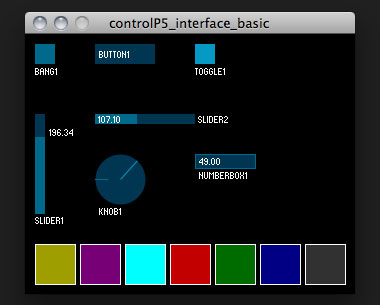
\includegraphics[width=8cm]{gambar/controlp5.jpg}
	\caption{Grafik Pengujian Koordinat X}
	\label{pic.koordinatx}
\end{figure}

Dari hasil pengujian yang ditampilkan pada Tabel \ref{tbl.koordinatx} dan juga Gambar \ref{pic.koordinatx} terlihat bahwa posisib \textit{end-effector} yang dihasilkan pada robot SCARA dibandingkan dengan data sesuai perhitungan kinematika memiliki sedikit perbedaan pada beberapa data. Perbedaan data ini dapat ditolerasi karena dengan \textit{sampling} koordinat X yang diuji hanya kurang dari lima persen nilai data yang berbeda. Pada hasil yang ditunjukkan diketahui bahwa posisi \textit{end-effector} memiliki batas minimum dan juga maksimum. Batas minimum posisi \textit{end-effector} pada sumbu X yaitu 10 cm dari titik pusat dan batas maksimum posisi \textit{end-effector} pada posisi sumbu X adalah 60 cm yang merupakan panjang dari lengan \textit{shoulder} dan juga lengan \textit{elbow}. 

\subsubsection{Pengujian Koordinat Y}
Pengujian koordinat Y dilakukan untuk mengetahui batas minimal dan batas maksimal \textit{end-effector} dari \textit{arm manipulator} robot SCARA relatif terhadap sumbu Y. Pengujian koordinat Y dilakukan dengan cara mengujicobakan setiap titik dari 0 cm sampai dengan total panjang \textit{shoulder} dan \textit{elbow} yaitu 60 cm menggunakan perhitungan kinematika balik. Perhitungan posisi Y diujicobakan menggunakan program Processing IDE, sementara untuk pengukuran posisi diukur secara faktual dari posisi \textit{end-effector} dengan membuat sebuah diagram kartesius. Tabel \ref{tbl.koordinaty} menunjukkan pengujian koordinat Y dan Gambar \ref{pic.koordinaty} menunjukkan grafik dari sampling koordinat Y.
 \begin{table}[H]
 	\centering
 	\caption{Hasil Pengujian Koordinat X}
 	\label{tbl.koordinaty}
 	\begin{tabular}{|c|l|}
 		\hline
 		\rowcolor[HTML]{9B9B9B} 
 		
 		No & \multicolumn{1}{c|}{\cellcolor[HTML]{9B9B9B}Keterangan} \\ \hline
 		1  & Robot Lengan SCARA                                      \\ \hline
 		2  & Box Panel                                               \\ \hline
 		3  & Arduino Mega 2560                                       \\ \hline
 		4  & Personal Computer                                       \\ \hline
 		5  & GUI Processing IDE                                      \\ \hline
 		6  & Workspace Robot SCARA                                   \\ \hline
 		7  & Kompresor                                               \\ \hline
 		8  & Objek                                                   \\ \hline
 	\end{tabular}
 	
 \end{table} 
 \begin{figure}[H]
 	\centering
 	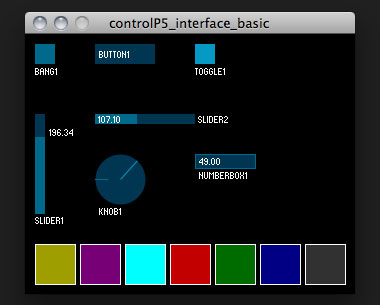
\includegraphics[width=8cm]{gambar/controlp5.jpg}
 	\caption{Grafik Pengujian Koordinat X}
 	\label{pic.koordinaty}
 \end{figure}


Dari hasil pengujian yang ditampilkan pada Tabel \ref{tbl.koordinaty} dan juga Gambar \ref{pic.koordinaty} terlihat bahwa posisi \textit{end-effector} yang dihasilkan pada robot SCARA dibandingkan dengan data sesuai perhitungan kinematika memiliki sedikit perbedaan pada beberapa data. Perbedaan data ini dapat ditolerasi karena dengan \textit{sampling} koordinat Y yang diuji hanya kurang dari lima persen nilai data yang berbeda. Pada hasil yang ditunjukkan diketahui bahwa posisi \textit{end-effector} memiliki batas minimum dan juga maksimum. Batas minimum posisi \textit{end-effector} pada sumbu Y yaitu 0 cm dari titik pusat dan batas maksimum posisi \textit{end-effector} pada posisi sumbu X adalah 60 cm yang merupakan panjang dari lengan \textit{shoulder} dan juga lengan \textit{elbow}. 

\subsubsection{Pengujian \textit{Joint Shoulder}}
Pengujian \textit{joint shoulder} dilakukan dengan membandingkan nilai sudut yang dihasilkan oleh perhitungan kinematika yang ada pada program processing IDE dengan sudut yang dihasilkan dalam aktual robot SCARA. Pengujian dilakukan dengan cara memberikan sebuah posisi koordinat X dan Y dengan nilai yang bervariasi. Nilai tersebut dimasukkan ke dalam sebuah perhitungan kinematika balik yang ada pada program Processing IDE. Hasil yang dihasilkan oleh perhitungan merupakan nilai sudut dari \textit{joint shoulder} dan juga \textit{elbow}. Perhitungan aktual dilakukan dengan cara mengukur sudut pada setiap \textit{joint} menggunakan bantuan busur atau \textit{software} sensor kemiringan yang di-\textit{install} pada smartphone. Tabel \ref{tbl.jointshoudler} merupakan hasil pengujian dari \textit{joint shoulder} berdasarkan \textit{sampling} posisi yang diambil. Gambar \ref{pic.jointshoulder} merupakan grafik hubungan dari sudut aktual dan sudut berdasarkan perhitungan kinematika. 

\begin{table}[H]
	\centering
	\caption{Hasil Pengujian \textit{Joint Shoulder}}
	\label{tbl.jointshoulder}
	\begin{tabular}{|c|l|}
		\hline
		\rowcolor[HTML]{9B9B9B} 
		
		No & \multicolumn{1}{c|}{\cellcolor[HTML]{9B9B9B}Keterangan} \\ \hline
		1  & Robot Lengan SCARA                                      \\ \hline
		2  & Box Panel                                               \\ \hline
		3  & Arduino Mega 2560                                       \\ \hline
		4  & Personal Computer                                       \\ \hline
		5  & GUI Processing IDE                                      \\ \hline
		6  & Workspace Robot SCARA                                   \\ \hline
		7  & Kompresor                                               \\ \hline
		8  & Objek                                                   \\ \hline
	\end{tabular}
	
\end{table} 
\begin{figure}[H]
	\centering
	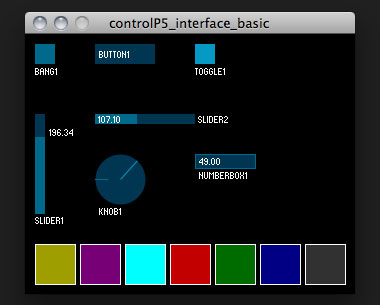
\includegraphics[width=8cm]{gambar/controlp5.jpg}
	\caption{Grafik Pengujian \textit{Joint Shoulder}}
	\label{pic.jointshoulder}
\end{figure}

Pada hasil yang ditunjukkan oleh Tabel \ref{tbl.jointshoulder} dan Gambar \ref{pic.jointshoulder} terlihat bahwa secara keseleuruhan nilai sudut yang dihasilkan oleh aktual pada robot SCARA dibandingkan dengan perhitungan kinematika oleh Processing IDE tidak begitu terdapat perbedaan. Terlihat bahwa nilai error
 memiliki nilai minimum .... persen dan nilai maksimum ... persen. Persentase error didapat dari data yang tidak sesuai dibagi oleh keleluruhan data yang diuji coba. 
 
 \subsubsection{Pengujian \textit{Joint Elbow}}
 Pengujian \textit{joint elbow} dilakukan dengan membandingkan nilai sudut yang dihasilkan oleh perhitungan kinematika yang ada pada program processing IDE dengan sudut yang dihasilkan dalam aktual robot SCARA. Pengujian dilakukan dengan cara memberikan sebuah posisi koordinat X dan Y dengan nilai yang bervariasi. Nilai tersebut dimasukkan ke dalam sebuah perhitungan kinematika balik yang ada pada program Processing IDE. Hasil yang dihasilkan oleh perhitungan merupakan nilai sudut dari \textit{joint shoulder} dan juga \textit{elbow}. Perhitungan aktual dilakukan dengan cara mengukur sudut pada setiap \textit{joint} menggunakan bantuan busur atau \textit{software} sensor kemiringan yang di-\textit{install} pada smartphone. Tabel \ref{tbl.jointelbow} merupakan hasil pengujian dari \textit{joint elbow} berdasarkan \textit{sampling} posisi yang diambil. Gambar \ref{pic.jointelbow} merupakan grafik hubungan dari sudut aktual dan sudut berdasarkan perhitungan kinematika. 
 
 \begin{table}[H]
 	\centering
 	\caption{Hasil Pengujian \textit{Joint Elbow}}
 	\label{tbl.jointelbow}
 	\begin{tabular}{|c|l|}
 		\hline
 		\rowcolor[HTML]{9B9B9B} 
 		
 		No & \multicolumn{1}{c|}{\cellcolor[HTML]{9B9B9B}Keterangan} \\ \hline
 		1  & Robot Lengan SCARA                                      \\ \hline
 		2  & Box Panel                                               \\ \hline
 		3  & Arduino Mega 2560                                       \\ \hline
 		4  & Personal Computer                                       \\ \hline
 		5  & GUI Processing IDE                                      \\ \hline
 		6  & Workspace Robot SCARA                                   \\ \hline
 		7  & Kompresor                                               \\ \hline
 		8  & Objek                                                   \\ \hline
 	\end{tabular}
 	
 \end{table} 
 \begin{figure}[H]
 	\centering
 	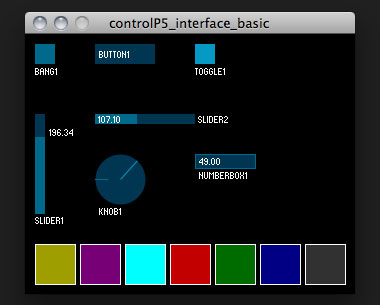
\includegraphics[width=8cm]{gambar/controlp5.jpg}
 	\caption{Grafik Pengujian \textit{Joint Elbow}}
 	\label{pic.jointelbow}
 \end{figure}
 
 Pada hasil yang ditunjukkan oleh Tabel \ref{tbl.jointelbow} dan Gambar \ref{pic.jointelbow} terlihat bahwa secara keseleuruhan nilai sudut yang dihasilkan oleh aktual pada robot SCARA dibandingkan dengan perhitungan kinematika oleh Processing IDE tidak begitu terdapat perbedaan. Terlihat bahwa nilai error
 memiliki nilai minimum .... persen dan nilai maksimum ... persen. Persentase error didapat dari data yang tidak sesuai dibagi oleh keleluruhan data yang diuji coba. 
 \subsection{Pengujian GUI}
 Pengujian GUI dilakukan untuk membandingkan posisi dari aktual robot SCARA dengan posisi yang ada pada Processing IDE. Pengujian dilakukan dengan memberikan \textit{sampling} posisi yang kemudian dilihat posisi dari robot secara aktual maupun Processing IDE. Gambar \ref{pic.pengujiangui1}, Gambar \ref{pic.pengujiangui2}, dan Gambar \ref{pic.pengujiangui3} merupakan hasil sampling perbandingan posisi dari robot SCARA secara aktual dan secara animasi.
  \begin{figure}[H]
 	\centering
 	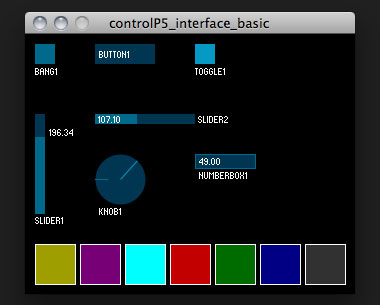
\includegraphics[width=8cm]{gambar/controlp5.jpg}
 	\caption{Perbandingan Gambaran Robot SCARA}
 	\label{pic.pengujiangui1}
 \end{figure}
\begin{figure}[H]
	\centering
	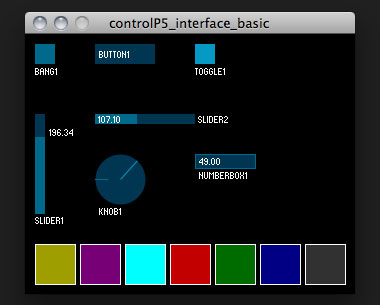
\includegraphics[width=8cm]{gambar/controlp5.jpg}
	\caption{Perbandingan Gambaran Robot SCARA}
	\label{pic.pengujiangui2}
\end{figure}
\begin{figure}[H]
	\centering
	\includegraphics[width=8cm]{gambar/controlp5.jpg}
	\caption{Perbandingan Gambaran Robot SCARA}
	\label{pic.pengujiangui3}
\end{figure}
Dari hasil yang ditunjukkan oleh Gambar \ref{pic.pengujiangui1}, Gambar \ref{pic.pengujiangui2}, dan Gambar \ref{pic.pengujiangui3} terlihat bahwa perbedaan posisi dari robot SCARA aktual dan pada Processing IDE hanya beberapa dan dapat ditoleransi, Terlihat bahwa posisi yang ditunjukkan oleh robot SCARA aktual dan robot SCARA processing IDE selalu sama. Sudut dari \textit{shoulder} dan \textit{elbow} yang masing-masing ditunjukkan terlihat sama meskipun ada sedikit perbedaan yang masih dapat ditoleransi.

\section{Pengujian Keseluruhan}
Setelah semua komponen sistem yang diuji dapat bekerja dengan baik, pengujian selanjutnya adalah pengujian sistem secara keseluruhan dengan beberapa parameter uji yang diberikan. Parameter uji tersebut diantaranya adalah pengujian akurasi robot lengan, dan simulasi robot lengan. 

\subsection{Pengujian Akurasi Robot Lengan}
Pada pengujian akurasi robot lengan dilakukan pengujian dengan memberikan posisi koordinat X dan Y dan melihat kembali posisi X dan Y secara aktual, melihat besar sudut pada masing-masing joint dengan perbandingan perhitungan kinematika. Pengujian akurasi robot lengan ini akan menghasilkan sebuah hasil secara luas dan dapat ditarik untuk sebuah kesimpulan yang menentukan robot SCARA dapat bekerja baik atau buruk secara keseluruhan. Tabel \ref{tbl.akurasikeseluruhan} merupakan hasil dari pengujian akurasi robot lengan secara keseluruhan. Gambar \ref{pic.akurasikeseluruhan} merupakan grafik dari hasil pengujian akurasi robot lengan secara keseluruhan.

\begin{table}[H]
	\centering
	\caption{Hasil Pengujian Akurasi Robot Secara Keseluruhan}
	\label{tbl.akurasikeseluruhan}
	\begin{tabular}{|c|l|}
		\hline
		\rowcolor[HTML]{9B9B9B} 
		
		No & \multicolumn{1}{c|}{\cellcolor[HTML]{9B9B9B}Keterangan} \\ \hline
		1  & Robot Lengan SCARA                                      \\ \hline
		2  & Box Panel                                               \\ \hline
		3  & Arduino Mega 2560                                       \\ \hline
		4  & Personal Computer                                       \\ \hline
		5  & GUI Processing IDE                                      \\ \hline
		6  & Workspace Robot SCARA                                   \\ \hline
		7  & Kompresor                                               \\ \hline
		8  & Objek                                                   \\ \hline
	\end{tabular}
	
\end{table} 
\begin{figure}[H]
	\centering
	\includegraphics[width=8cm]{gambar/controlp5.jpg}
	\caption{Grafik Pengujian Akurasi Robot Secara Keseluruhan}
	\label{pic.akurasikeseluruhan}
\end{figure}

Pada hasil pengujian yang ditunjukkan pada Tabel \ref{tbl.akurasikeseluruhan} dan Gambar \ref{pic.akurasikeseluruhan} terlihat bahwa pengujian mendapat beberapa data yang beragam. Terlihat bahwa nilai kekeliriuan paling banyak terdapat pada bagian posisi koordinat X dan Y dan ekeliuran paling sedikit pada bagian sudut shoulder. Sedangkan untuk sistem keseluruhan kekeliruan total pada akurasi robot memiliki nilai ... persen. Nilai sebesar ini merupakan nilai yang cukup baik bagi sebuah sistem. Dengan nilai tersebut maka sistem kinematika robot SCARA ini dapat dikatakan baik. 

%BAB_5 LAPORAN KP

\chapter{PENUTUP}
\section{Kesimpulan}
Dari hasil pengujian dan pembahasan terhadap alat dan sistem “Kinematika dan Antarmuka Robot SCARA berbasis Processing IDE” yang telah dirancang dan dibuat ini, maka dapat disimpulkan sebagai berikut:
\begin{enumerate}
	\item Sistem kendali robot lengan dengan Arduino Mega 2560 dapat digunakan dengan baik dan dapat menerapkan sistem kinematika denga benar. Hasil dari nilai data yang diperoleh pada Processing IDE selanjutnya digunakan sebagai masukan untuk kinematika balik yang hasilnya dikirimkan pada Arduino Mega 2560 yang diteruskan pada motor DC.
	\item GUI yang dibuat sebagai jembatan antara user dengan hardware memiliki beberapa masukan data dan juga tampilan data berupa animasi dari robot SCARA.
	\item Implementasi dari kineatika robot SCARA dapat berjalan dengan baik meskipun terdapat beberapa data yang tidak akurat. 
	\item  Hal-hal yang menyebabkan robot lengan SCARA  tidak akurat dalam menentukan posisi end-effector diantaranya sebagai berikut:
	\subitem   Terdapat toleransi sudut pada joint shoulder dan joint elbow dan elbow yang menyebabkan $\theta_{1}, \theta_{2}$, memiliki nilai toleransi sebesar 3 derajat. 
	\subitem  Kepresisian  pembacaan nilai analog potensiometer pada feedback posisi. 
\end{enumerate}
\section{Saran}
Setelah mengambil beberapa kesimpulan dan melihat dari sistem secara keseluruhan, terdapat beberapa saran disampaikan untuk menambah mutu dan kualitas dari sistem kendali robot lengan SCARA adalah sebagai berikut: 
\begin{enumerate}
	\item Untuk menghasilkan kinematika yang baik maka toleransi besar sudut pada motor DC bisa diperkecil dan ditambahkan PID
	\item Untuk menghasilkan tampilan yang nyata maka pada sistem diberi tambahan kamera yang dapat ditampilan pada GUI
\end{enumerate}

\bibliography{IEEEabrv,references}
\addcontentsline{toc}{chapter}{DAFTAR PUSTAKA}

\end{document}